\documentclass[a4paper,12pt,twoside]{book}

\sloppy
% \frenchspacing
\setlength{\unitlength}{1cm}
% Do not change following line pdfmanual depends on it!
\input{pdfswitch}
%\usepackage{pdfcolmk}
\usepackage{verbatim}
\usepackage{cite}

\usepackage{graphicx}
\usepackage{amsmath}
\usepackage{amssymb}
\usepackage{amsfonts}
\usepackage{mathrsfs}
\usepackage{a4wide}
\usepackage{fancyheadings}
\usepackage[footnotesize,bf]{caption}
\usepackage{makeidx}
%Preparations for multiple indices
\usepackage{multind}


%%%%%%%%%%%%%%%%%%%%%%%%%%%%%%%%%%%%%%%%
\usepackage{ae,aecompl} % only for Type 1 fonts for readable pdf convert; may not be necessary anymore!

\newcommand{\glbxxx}{hep-ph/0407333}
\newcommand{\glbxxxtwo}{hep-ph/0701187}
\newcommand{\capdef}{}
\newcommand{\mycaption}[2][\capdef]{\renewcommand{\capdef}{#2}%
        \caption[#1]{{ %\itshape
 {\footnotesize #2}}}}
\makeatletter
\renewcommand{\fnum@table}{\textbf{\tablename~\thetable}}
\renewcommand{\fnum@figure}{\textbf{\figurename~\thefigure}}
\makeatother

% Index: use "makeindex Manual" to create .ind file
%\makeindex

\makeindex{norm}
\makeindex{constants}
\makeindex{api}
\makeindex{aedl}

\newcommand{\bi}{\begin{itemize}}
\newcommand{\ei}{\end{itemize}}
\newcommand{\ra}{$\rightarrow$}
\newcommand{\be}{\begin{equation}}
\newcommand{\ee}{\end{equation}}
\newcommand{\bea}{\begin{eqnarray}}
\newcommand{\eea}{\end{eqnarray}}
\newcommand{\nn}{\nonumber}
\newcommand{\ldm}{\Delta m_{31}^2}
\newcommand{\sdm}{\Delta m_{21}^2}
\newcommand{\deltacp}{\delta_{\mathrm{CP}}}
\newcommand{\stheta}{\sin^2 2 \theta_{13}}

\newcommand{\ie}{{\it i.e.}}
\newcommand{\Ie}{{\it I.e.}}
\newcommand{\eg}{{\it e.g.}}
\newcommand{\Eg}{{\it E.g.}}
\newcommand{\cf}{{\it cf.}}
\newcommand{\etc}{{\it etc.}}
\newcommand{\eq}{Eq.}
\newcommand{\eqs}{Eqs.}
\newcommand{\Def}{Definition}
\newcommand{\fig}{Fig.}
\newcommand{\Fig}{Fig.}
\newcommand{\figs}{Figs.}
\newcommand{\Figs}{Figs.}
\newcommand{\Ref}{Ref.}
\newcommand{\Refs}{Refs.}
\newcommand{\Sec}{Sec.}
\newcommand{\Secs}{Secs.}
\newcommand{\Chapt}{Chapter}
\newcommand{\Chapts}{Chapters}
\newcommand{\Part}{Part}
\newcommand{\App}{Appendix}
\newcommand{\Apps}{Appendices}
\newcommand{\Tab}{Table}
\newcommand{\Tabs}{Tables}

\newcommand{\JHFSK}{{\sc JHF-SK}}
\newcommand{\NUMI }{{\sc NuMI}}
\newcommand{\ReactorI}{{\sc Reactor-I}}
\newcommand{\ReactorII}{{\sc Reactor-II}}
\newcommand{\JHFHK}{{\sc JHF-HK}}
\newcommand{\NuFactI}{{\sc NuFact-I}}
\newcommand{\NuFactII}{{\sc NuFact-II}}
\newcommand{\SPL}{{\sc SPL}}
\newcommand{\Beta}{{\sc $\beta$-Beam}}
\newcommand{\NOVA}{{\sc NO$\nu$A}}
\newcommand{\TtoK}{{\sc T2K}}
\newcommand{\TtoHK}{{\sc T2HK}}
\newcommand{\DC}{{Double\sc Chooz}}

\newcommand{\GLOBES}{{\sf GLoBES}}
\newcommand{\AEDL}{{\sf AEDL}}
\newcommand{\EDM}{{\sf EDM}}

\newcommand{\equ}[1]{\eq~(\ref{equ:#1})}
\newcommand{\figu}[1]{\fig~\ref{fig:#1}}
\newcommand{\tabl}[1]{\Tab~\ref{tab:#1}}
\newcommand{\tb}{\hspace*{3ex}}

% Set as GLoBES command and add to index:
% Always use GLB when mentioning a command in text!
\newcommand{\GLB}[1]{{\tt glb#1}\index{api}{#1@{\tt #1}}}
% Always use GLBNS when adding a command to the index without showing it!
\newcommand{\GLBNS}[1]{\index{api}{#1@{\tt #1}}}

% Set as GLoBES command and add to index:
% Always use GLB when mentioning a command in text!
\newcommand{\GLBC}[1]{{\tt #1}\index{constants}{\tt{#1}}}
% Always use GLBNS when adding a command to the index without showing it!
\newcommand{\GLBNSC}[1]{\index{constants}{{\tt #1}}}
\newcommand{\gq}[1]{\begin{quote} {\tt #1} \end{quote}}
\newcommand{\go}[1]{$\rightarrow$ Output: \begin{quote} {\sf #1} \end{quote}}
\newcommand{\bugs}{{\tt globes@ph.tum.de}}
\definecolor{light}{gray}{0.93}
\definecolor{heavy}{gray}{0.35}
\setlength{\fboxrule}{0.1cm}
\newcommand{\example}[2]{
\begin{table}[p]
\begin{center}
\fcolorbox{heavy}{light}{
\begin{minipage}[t][\textheight][t]{15.5cm}
{\em \underline{Example:} #1}

\vspace*{0.3cm}

#2

\end{minipage}
}
\end{center}
\end{table}
}


\newtheorem{function}{Function}[chapter]

%-- page parameters -------------------------------------------------

\pagestyle{fancyplain}

% Olddefs:

%\addtolength{\textwidth}{-1truecm}
%\addtolength{\oddsidemargin}{1.0truecm}
%\addtolength{\evensidemargin}{-0.3truecm}

% Owndefs:

%\addtolength{\textwidth}{0.0truecm}
%\addtolength{\textheight}{1.8truecm}
%\addtolength{\topmargin}{-0.6truecm}
%\addtolength{\oddsidemargin}{0.65truecm}
%\addtolength{\evensidemargin}{-1.0truecm}

% Headdefs:

\advance \headheight by 3.0truept       % for 12pt mandatory...
\lhead[\fancyplain{}{\thepage}]{\fancyplain{}{\rightmark}}
\rhead[\fancyplain{}{\leftmark}]{\fancyplain{\thepage}{\thepage}}
\cfoot{}

\renewcommand{\chaptermark}[1]{
% chapter title im Seitenkopf
\markboth{\uppercase{\chaptername}\ \thechapter.\ \ #1}
          {\uppercase{\chaptername}\ \thechapter.\ \ #1}}
% section title im Seitenkopf
\renewcommand{\sectionmark}[1]{\markright{\thesection\ \ #1}}




\begin{document} 

\frontmatter
\pagenumbering{Roman}
\thispagestyle{empty}
{
\setlength{\parindent}{0cm}

%\begin{titlepage}

\font\fa=cmssbx14 scaled 1440
\font\fb=cmbx10 scaled 1200
\font\fc=cmb10 scaled 1200
\font\fd=cmr10 scaled 1000  

{\setlength{\baselineskip}{1.2cm}}

\vspace*{1.5cm}

\begin{center}
{ \Large \bf
{\Huge \GLOBES} \\
General Long Baseline Experiment Simulator \\ }
\vspace*{0.5cm}
{\large \bf User's and experiment definition manual }

%\vspace*{1.5cm}
%{\large \bf !!!DRAFT IN PROGRESS!!! }
\end{center}

\vspace{0.5cm}

\begin{center}
{\large Patrick Huber$^a$, Joachim Kopp$^b$, Manfred Lindner$^b$, \\ Mark Rolinec$^c$, Walter Winter$^d$}
\end{center}

\vspace{0.3cm}

\begin{center}





\end{center}

\vspace{0.5cm}

\begin{center}
\colorbox{black}{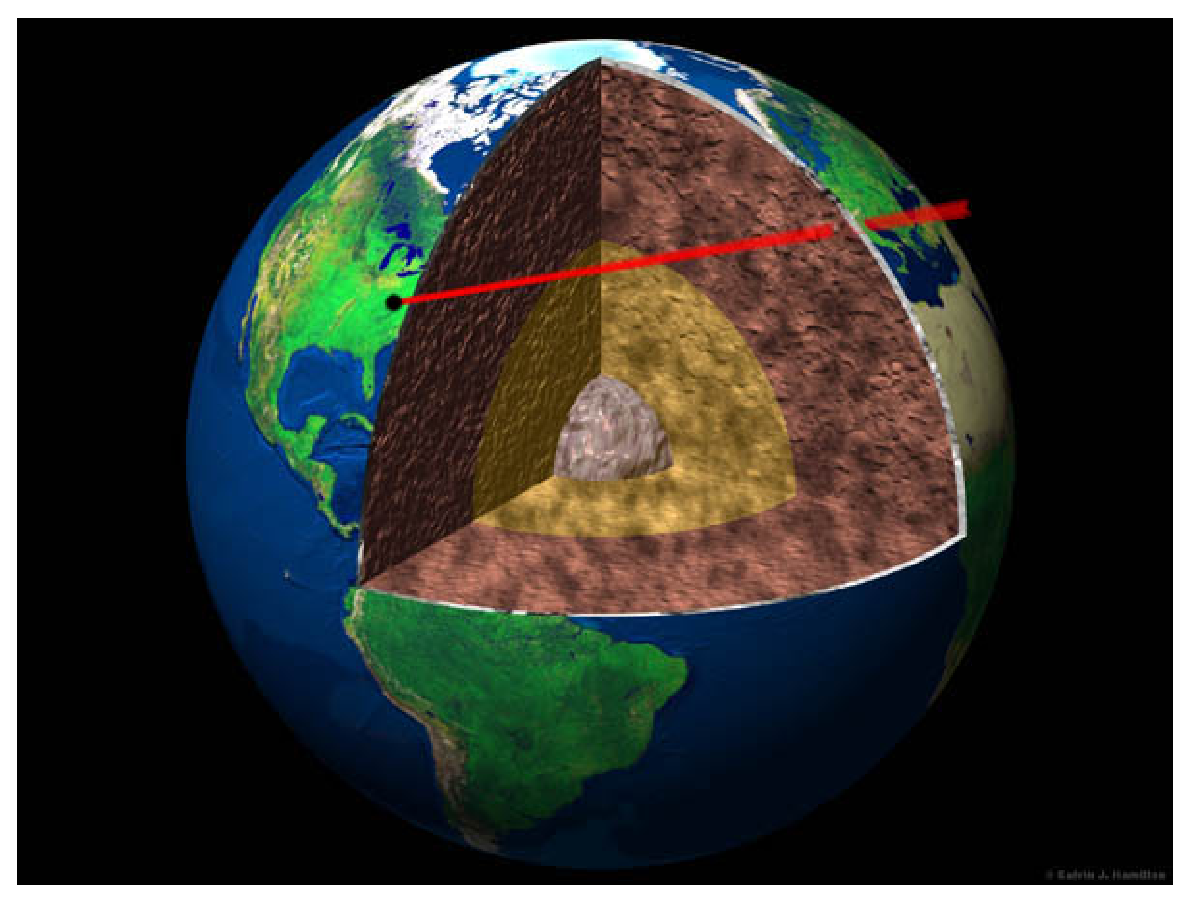
\includegraphics[width=7cm]{.save/earthint}}

\vspace*{-1cm}

{\Huge \textcolor{yellow}{GLoBES}}
\end{center}

\vspace{1cm}

\begin{center}
Version from \today\ for \GLOBES\ 3.0
\end{center}


\vspace*{0.5cm}
\vfill
\hrule

\vspace*{0.1cm}

{\em\small $^{\mathrm{a}}$%
       University of Wisconsin,  Physics Department,
       1150 University Av., Madison, WI 53706, USA}

{\em\small $^{\mathrm{b}}$%
       Max--Planck--Institut f\"ur Kernphysik, 
       Postfach 10~39~80, D--69029 Heidelberg, Germany} 

{\em\small $^{\mathrm{c}}$%
       Technische Universit\"at M\"unchen,
       Institut f\"ur Theoretische Physik, Physik--Department,\\
       James--Franck--Strasse, D--85748 Garching, Germany}

{\em\small $^{\mathrm{d}}$%
       Universit\"at W\"urzburg, 
       Lehrstuhl f\"ur theoretische Physik II, \\
       Institut f\"ur theoretische Physik und Astrophysik, 
       Am Hubland,
       D-97074 W\"urzburg, Germany}

%\end{titlepage}

%\title{}
%\date{}
%\author{}
%\maketitle

}


\clearpage
\thispagestyle{empty}
\bigskip
\begin{quote}
    Copyright \copyright  2004--2007  The GLoBES Team.
    Permission is granted to copy, distribute and/or modify this document
    under the terms of the GNU Free Documentation License, Version 1.2
    or any later version published by the Free Software Foundation;
    with the invariant Sections ``Terms of usage of \GLOBES" 
    and ``Acknowledgments'', no Front-Cover Texts, and no Back-Cover Texts.
    A copy of the license is included in the section entitled "GNU
    Free Documentation License".
\end{quote}
\bigskip
    


\cleardoublepage
\setcounter{page}{1}

\chapter*{What is \GLOBES ?}

\vspace*{-4ex}
\GLOBES\ (``General Long Baseline Experiment Simulator'') is a flexible
software package to simulate neutrino oscillation 
long baseline and reactor experiments. On the
one hand, it contains a comprehensive abstract experiment definition
language (\AEDL), which allows to describe most classes 
of long baseline experiments
at an abstract level. On the other hand, it provides a C-library to
process the experiment information in order to obtain oscillation
probabilities, rate vectors, and $\Delta \chi^2$-values. Currently, 
\GLOBES\ is available for GNU/Linux. Since the source code is included,
the port to other operating systems is in principle possible. The software
as well as up-to-date versions of this manual can be found at this URL:
 \verb+http://www.mpi-hd.mpg.de/~globes+

\GLOBES\ allows to simulate experiments with stationary neutrino point sources, where each experiment is assumed to have only one neutrino source.
Such experiments are neutrino beam experiments and reactor experiments. 
Geometrical effects of a source distribution, such as in the sun or the 
atmosphere, can not be described. In addition, sources with a physically 
significant time dependence, such as supernov\ae, can not be studied. It 
is, however, possible to simulate beams with bunch structure, since the 
time dependence of the neutrino source is physically only important to suppress backgrounds. 
Furthermore, experiments with discrete numbers of sources and detectors can
be implemented by user-defined systematics in \GLOBES\ 3.0 and higher.

On the experiment definition side, either built-in neutrino fluxes
(\eg, neutrino factory, $\beta$-Beam) or arbitrary fluxes can be used. Similarly,
arbitrary cross sections, energy dependent efficiencies, the
energy resolution function, the considered oscillation channels, 
backgrounds, and many other features can be specified. 
For the systematics, energy
normalization and calibration errors can be simulated in a straightforward way,
or the systematics can be completely user-defined (Version 3.0 and higher). Note that
the energy ranges and windows, as well as the bin widths can be
(almost) arbitrarily chosen, which means that variable bin
widths are allowed. Together with \GLOBES\ comes a number of
pre-defined experiments in order to demonstrate the capabilities
of \GLOBES\ and to provide prototypes for new experiments.

With the C-library, one can extract the $\Delta \chi^2$ for all defined 
oscillation channels for an experiment or any combination of experiments.
Of course, also low-level information, such as oscillation
probabilities or event rates, can be obtained. \GLOBES\ includes the
simulation of neutrino oscillations in matter with arbitrary matter 
density profiles, as well as it allows to simulate the matter density
uncertainty. As one of the most
advanced features of \GLOBES , it provides the technology to 
project the $\Delta \chi^2$, which is a function of all oscillation
parameters, onto any subspace of parameters by local minimization. 
This approach allows the inclusion of multi-parameter-correlations,
where external input (\eg, from solar experiments) can be imposed, too.
Applications of the projection mechanism include the projections onto the $\stheta$-axis and the $\stheta$-$\deltacp$-plane. In addition, all oscillation parameters can be kept free to precisely localize 
degenerate solutions.

In the newest version \GLOBES\ 3.0 flexibility is introduced at all levels. At the probability level,
the transition probabilities can be modified to introduce new physics. At the systematics level,
user-defined systematical errors and correlations between sources or detectors can be simulated,
and at the analysis level, arbitrary  input from external measurements can be added.
Therefore, \GLOBES\ now provides solutions for new classes of problems.

\chapter*{Terms of usage of \GLOBES}

\subsection*{Referencing the \GLOBES\ software}

\GLOBES\ is developed for academic use. Thus, the \GLOBES\ Team would
appreciate being given academic credit for it. Whenever you use \GLOBES\
to produce a publication or a talk indicate that you have used \GLOBES\ and
please cite the following references~\cite{globes_paper,globes_paper_two}
\begin{quote}
P. Huber, M. Lindner and W. Winter\\
Simulation of long baseline neutrino oscillation experiments with \GLOBES ,\\
Comput. Phys. Commun. 167 (2005) 195, arXiv:\glbxxx,
\end{quote}

\begin{quote}
P. Huber, J. Kopp, M. Lindner, M. Rolinec, and W. Winter\\
 New features in the simulation of neutrino oscillation experiments with \GLOBES~3.0,
arXiv:\glbxxxtwo,
\end{quote}
but \emph{not} this manual. This manual itself is not a scientific 
publication and will not be submitted to a scientific journal. 
It will evolve during time since it is intended for 
regular revision. Besides that, many of the data which are used by \GLOBES\ 
and distributed together with it should be properly referenced. 
For details see below.

Apart from that, \GLOBES\ is free software and open source, \ie, it is 
licensed under the GNU Public License.

\subsection*{Referencing the data in \GLOBES}
\label{ref_data}

\index{norm}{Referencing!data in \GLOBES}
\GLOBES\ wouldn't be useful without having high quality input data.
Much of these input data have been published elsewhere and the authors
of those publications would appreciate to be cited whenever their work
is used. It is solely the user's responsibility 
to make sure that he understands where the input material for \GLOBES\ comes
from and if additional work has to be cited in addition to the 
\GLOBES\ papers~\cite{globes_paper,globes_paper_two}. To assist with this task, we provide  the necessary information for the data coming along together with \GLOBES.

When using the built-in Earth matter density profile, the 
original source is \Refs~\cite{Dziewonski:1981xy,Stacey}.

All files ending with \verb+.dat+ or \verb+.glb+ 
in the \verb+data+ subdirectory of the \GLOBES\ tar-ball have on top a comment field which clearly indicates which studies should be
cited when using a certain file. Make sure that dependencies are correctly
tracked, \ie , in some cases files included by other files need to be 
checked, too (for example, cross section or flux files). One can use 
the \verb+-v3+ option to the \verb+globes+ command to see which files
are included (\cf, \Chapt~\ref{chap:exp_def}).
It is recommended that you use the same style for your own input files, since then, in case they are distributed, everybody will know how to correctly reference your work.

\chapter*{What is new in \GLOBES ?}

Here we briefly summarize the main changes of the new GLoBES version. For details, please
refer to the respective parts of the manual. Please note that any new \GLOBES\ version is
compatible with older versions, \ie, old application software and \AEDL\ files should, with minor
modifications, run with the new version as well.  However, some function names and features will
evolve during time, which means that outdated features may not be documented anymore.

\section*{Version 3.0}
\index{norm}{Version 3.0}

Here comes a summary of the most important changes in this version for users of earlier
versions of \GLOBES .

\subsection*{New features}

\begin{itemize}
 \item
  User-defined systematics, which can be used to simulate reactor experiments \etc ; see \Secs~\ref{sec:userchi}
and~\ref{sec:rules}
 \item
  User-defined priors to include arbitrary external information in the $\chi^2$ before
marginalization over the oscillation parameters; see \Sec~\ref{sec:userdefined} 
\item
  Non-standard physics support; see \Chapt~\ref{chapt:nsphysics}
\item
  Beta beam fluxes available as built-in fluxes; see \Sec~\ref{sec:source}
\item
  Enhanced support for parallelization, such as Condor; see, \eg, page~\pageref{sec:condor}
\item
  Updated \AEDL\ files; see \Tab~\ref{tab:experiments}
\item
 New \AEDL\ features, such as the support of lists as variables and an interpolation
routine; see \Sec~\ref{sec:advaedl}
\item
 Clean-up of inconsistencies, such as an overall (internal) normalization factor in the flux files;
see, \eg, page~\pageref{app:flux}
\item
  Faster probability engine, easier installation (internal changes)
\item
  Experimental feature: Alternative minimizer provided, which is usually faster than
the standard minimizer; see \Chapt~\ref{chapt:experimental}
\end{itemize}

\subsection*{Major changes}

Most of the modifications should not require that old pieces of software be changed. 
However, the following changes could be relevant:
\begin{itemize}
\item
 \GLB{SetDensityParams} has to be used with \GLB{DefineParams} and \GLB{SetDensityProjectionFlag} together
with \GLB{DefineProjection}, because unexpected pre-defined behavior should be avoided.
\item
 Functions \GLB{SetFilter}, \GLB{GetFilter}, \GLB{SetFilterState}, and \GLB{GetFilterState} replaced
by functions {\tt ...InExperiment}.
\item
 \AEDL\ requires now that {\tt \$version} be used to define the minimum version number this \AEDL\
file is to be used with. With this requirement one can easily avoid that new \AEDL\
files with new features be used with old versions of \GLOBES\ which may not recognize these features.
\item
 Some of the earlier \AEDL\ files have been updated, changed names, or have been removed. In addition, new files have been added. Although old \AEDL\ files will run as usual for compatibility, they will not be
supported by the \GLOBES\ Team anymore. You should make sure to keep these files when updating \GLOBES . 
\item 
 The implementation of the tilt (systematics) has slightly changed. The tilt also works for
variable bin widths. Therefore, you will obtain slightly different results when you run
the same \AEDL\ between older and newer versions of \GLOBES .
\end{itemize}

\subsection*{Minor changes}

Here we document the most important changes which should not affect older software:
\begin{itemize}
\item
 Functions and constants renamed for consistency:
\begin{itemize}
\item
 {\tt glbChiTheta} $\rightarrow$ {\tt glbChiTheta13}
\item
 {\tt glbChiThetaDelta} $\rightarrow$ {\tt glbChiTheta13Delta}
\item
 {\tt glbChiDms} $\rightarrow$ {\tt glbChiDm21}
\item
 {\tt glbChiDm} $\rightarrow$ {\tt glbChiDm31}
\item
 {\tt GLB\_DM\_SOL} $\rightarrow$ {\tt GLB\_DM\_21}
\item
 {\tt GLB\_DM\_ATM} $\rightarrow$ {\tt GLB\_DM\_31}
\item
 {\tt glbSetStartingValues} $\rightarrow$ {\tt glbSetCentralValues}
\item
 {\tt glbGetStartingValues} $\rightarrow$ {\tt glbGetCentralValues}
\item
 {\tt glbGetProfileData} $\rightarrow$ {\tt glbGetProfileDataInExperiment}
\end{itemize}
\item
 Rate access changed; see \Sec~\ref{sec:event_rates}
\item
 Systematics concept changed, concept of error dimensions removed; {\tt @backgroundcenter} removed, central values for all systematics parameters
now zero; see \Sec~\ref{sec:rules}
\end{itemize}

\cleardoublepage
\tableofcontents

\cleardoublepage
\setcounter{page}{1}
\pagenumbering{arabic}

\chapter*{How to use this manual}
\addcontentsline{toc}{chapter}{How to use this manual}

As it is illustrated in \figu{GLOBES}, \GLOBES\ consists 
of several modules.

\begin{figure}[bht]
\begin{center}
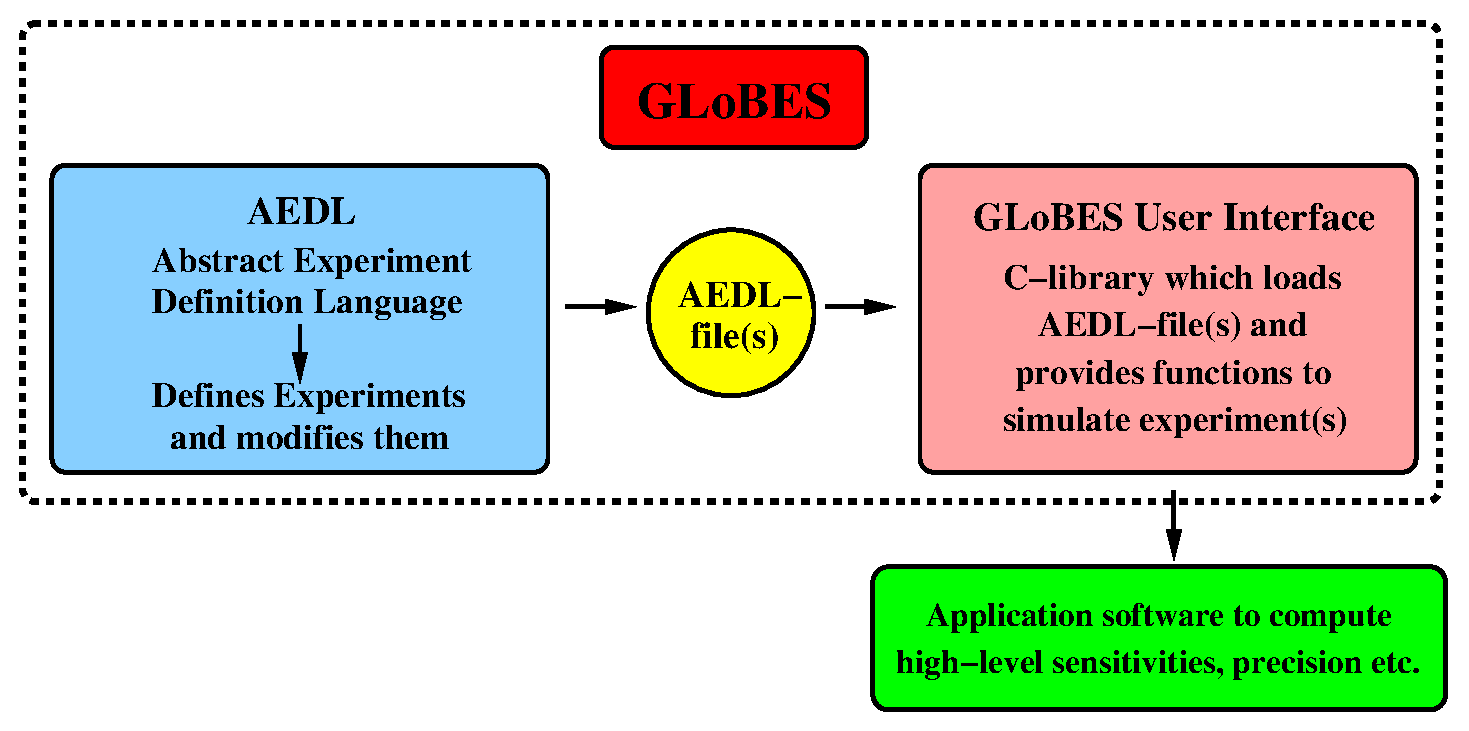
\includegraphics[width=16cm]{GLOBES}
\end{center}
\caption{\label{fig:GLOBES} Different modules in \GLOBES .}
\end{figure}
%
\AEDL (``Abstract Experiment Definition Language'') is a language
to define experiments in the form of ordinary text files. One or more of 
the resulting \AEDL\ files can then be processed together with supporting 
flux or cross section files by the user interface. The user interface
is a C-library, which loads one or more \AEDL\ file(s)
containing the experiment definition(s). The user interface is linked 
against the application software, and provides the user interface functions
for the intended experiment simulation. 

The application 
software is, except for some example files, not part of \GLOBES , since
the evaluation of the experiment performance is often a matter of taste
and definition. In addition, the algorithms depend, especially for
high-precision instruments, very much on the oscillation parameters.
In general, it is quite simple to simulate superbeams and reactor
experiments. However, because of the more complicated topology, the
simulation of neutrino factories is much more difficult. In order
to demonstrate some of these difficulties, we present in this manual mainly
examples with neutrino factories. These examples can be found in
\Part~\ref{part:1} within the boxed pages. As complete files, they
are also available in the \GLOBES\ software package.

The \GLOBES\ software may have two target groups: 
Physicists, who are mainly interested in optimizing the potential
of specific experimental setups, and others, who are mainly
interested in the physics potential of different experiment types
from a theoretical point of view.
For the first group, \AEDL\ could be the most interesting aspect of
\GLOBES , where the user interface is only a tool to obtain specific
parameter sensitivities. In this case, \GLOBES\ could serve as a
unified tool for the comparison and optimization of different experiment
 setups on equal footing, where
it is the primary objective to simulate the experiments as accurate
as possible. In addition, changes in experimental parameters, such as
efficiencies or energy resolutions, can quickly be tested.
%
For the second user group, the pre-defined 
experiment definition files might already be sufficient to test
new conceptual approaches, and the user interface is the most interesting
aspect for sophisticated applications including correlations,
degeneracies, and multi-experiment setups. In either case, the \GLOBES\
software could serve as a platform for the exchange of experiment
definitions, and for an efficient splitting of work between
experimentalists and theorists.

The user interface functions are described in \Part~\ref{part:1} of 
this manual, which is the ``user's manual''. In there, first of all a 
short \GLOBES\ tour is given in \Chapt~\ref{chapter:tour} in order to 
have an overview over \GLOBES .
After that, the user
interface is successively introduced from very basic to more sophisticated
functions. Eventually, it is demonstrated how one can change many
experiment parameters at running time (such as baseline or target mass), and how one can obtain low-level
information. We recommend that everybody interested in \GLOBES\ should
become familiar at least with the concepts in \Chapt~\ref{chapter:tour}
 and some of the examples on the boxed pages. The examples can be 
 directly compiled 
 from the respective directory in the \GLOBES\ software package.
The corresponding figures are produced with the
Mathematica Notebook {\tt DocPlots.nb}, which can be found
in the example directory as well.

In \Part~\ref{part:2} of the manual, \AEDL\ is described. After an
introductory chapter, all functions are defined in greater detail.
This part might be more interesting for the experimental users who
want to modify or create \AEDL\ files. A useful tool in this context
is the executable program \verb+globes+, which returns event rates and other
information for individual \AEDL\ files without further programming. 
For example, flux normalizations can with this tool be easily adjusted 
to reproduce the event rates of a specific experiment. It is described
in the last chapter of \Part~\ref{part:2}.

In this version of the manual, introductory topics and advanced topics are
mixed if they belong to the same subject. Therefore, we have marked more
advanced material by a star~($^*$). This material can be skipped in a first
reading of the manual. In some cases, it may be even recommendable to do
so because knowledge of \AEDL\ is required (which is introduced in
the second part).

% THE FOLLOWING HAS CHANGED: C99, COMPILED WITH GCC; MAYBE ONLY PROBLEMS WITH C89
%
% \paragraph{Note:} All examples for application software in C do require
% a C++ compiler to be properly compiled. For pedagogical reasons, variable
% declarations are done at that place where the variable is needed for the
% first time, which is at variance with C syntax but not with C++ syntax.
% That is the only way in which the examples deviate form ISO C. Moreover
% the actual numerical values of the results of the examples may be different
% from the ones in this manual.
%
% Comment by JK: A pedantic C89 compile will reject the example files (it would
% also reject GLoBES itself). With its default settings, gcc is relatively
% tolerant, so everything works with gcc. I assume that also the Intel
% compiler would be OK, but maybe Borland, Microsoft, or other compilers would
% produce problems.

\mainmatter
%%%%%%%%%%%%%%%%%%%%%%%%%%%%%%%%%%%
% PART I: User's manual
%%%%%%%%%%%%%%%%%%%%%%%%%%%%%%%%%%%

%%%%%%%%%%%%%%%%%%%%%%%%%%%%%%%%%%%
% PART I: User's manual
%%%%%%%%%%%%%%%%%%%%%%%%%%%%%%%%%%%

\part{User's manual}
\label{part:1}

\chapter{A \GLOBES\ tour}
\label{chapter:tour}
\index{GLoBES tour}

In this first chapter, we show a \GLOBES\ tour illustrating the
main features of \GLOBES . The complete example  
can be found as {\tt example-tour.c} in the example subdirectory of your \GLOBES\ distribution.
The output is written to {\tt stream}, which can be either {\tt stdout},
or a file. Details about how to use \GLOBES\ with C can found in \Chapt~\ref{chapt:gettingstarted} and the following chapters.
You can also find a summary of the most important \GLOBES\ $\chi^2$-functions in \tabl{stdfunctions}. Note that this chapter
can be skipped without loss of relevant information.

\begin{table}[tpb]
\begin{center}
\begin{tabular}{p{3.8cm}p{3.8cm}p{7cm}}
\hline
Function & Purpose & Parameters \ra\ Result \\
\hline
\multicolumn{3}{l}{{\bf Systematics only:}} \\
\GLB{glbChiSys} & $\chi^2$ with systematics only  & ({\tt glb\_params in, int exp, int rule}) \ra\  {\tt double} $\chi^2$ \\[0.2cm]
\multicolumn{3}{l}{{\bf Projections onto axes:}} \\
\GLB{glbChiTheta} & Projection onto $\theta_{13}$-axis  &  ({\tt glb\_params in, glb\_params out, int exp}) \ra\  {\tt double} $\chi^2$ \\[0.1cm]
\GLB{glbChiDelta} & Projection onto $\deltacp$-axis  &  ({\tt glb\_params in, glb\_params out, int exp}) \ra\  {\tt double} $\chi^2$ \\[0.1cm]
\GLB{glbChiTheta23} & Projection onto $\theta_{23}$-axis  &  ({\tt glb\_params in, glb\_params out, int exp}) \ra\  {\tt double} $\chi^2$ \\[0.1cm]
\GLB{glbChiDm} & Projection onto $\ldm$-axis  &  ({\tt glb\_params in, glb\_params out, int exp}) \ra\  {\tt double} $\chi^2$ \\[0.1cm]
\GLB{glbChiDms} & Projection onto $\sdm$-axis  &  ({\tt glb\_params in, glb\_params out, int exp}) \ra\  {\tt double} $\chi^2$ \\[0.2cm]
\multicolumn{3}{l}{{\bf Projection onto plane:}} \\
\GLB{glbChiThetaDelta} & Projection onto $\theta_{13}$-$\deltacp$-plane  &  ({\tt glb\_params in, glb\_params out, int exp}) \ra\  {\tt double} $\chi^2$ \\[0.2cm]
\multicolumn{3}{l}{{\bf Projection onto any hyper-plane:}} \\
\GLB{glbChiNP} & Projection onto any $n$-dimensional hyper-plane  &  ({\tt glb\_params in, glb\_params out, int exp}) \ra\  {\tt double} $\chi^2$ \newline
Needs \GLB{glbSetProjection} before! \\[0.2cm]
\multicolumn{3}{l}{{\bf Localization of degeneracies:}} \\
\GLB{glbChiAll} & (Local) Minimization over all parameters  &  ({\tt glb\_params in, glb\_params out, int exp}) \ra\  {\tt double} $\chi^2$ \\
\hline
\end{tabular}
\end{center}
\caption{\label{tab:stdfunctions} \index{Standard functions (table)} The \GLOBES\ standard function to obtain a $\chi^2$-value with systematics only or systematics and correlations. The parameters {\tt rule} and {\tt exp}
can either be \GLB{GLB\_ALL} for all initialized experiment or the
experiment number ($0$ to \GLB{glb\_num\_of\_exps}-1) for a specific experiment. The format of \GLB{glb\_params} is discussed in detail in \Chapt~\ref{chapt:gettingstarted}. Note that all functions but {\tt ChiSys}
  are using minimizers which have to be initialized with \GLB{glbSetInputErrors} and \GLB{glbSetStartingValues} first.}
\end{table}

\vspace*{0.5cm}

\noindent Initialize the \GLOBES\ library:
\gq{
glbInit(argv[0]);
} 
Define my standard oscillation parameters:
\gq{
double theta12 = asin(sqrt(0.8))/2; \\
double theta13 = asin(sqrt(0.001))/2;\\
double theta23 = M\_PI/4;\\
double deltacp = M\_PI/2;\\
double sdm = 7e-5;\\
double ldm = 2e-3;
}
Load one neutrino factory experiment:
\gq{
glbInitExperiment("NuFact.glb",\&glb\_experiment\_list[0], \\ \hspace*{4cm} \&glb\_num\_of\_exps);
} 
Initialize a number of parameter vectors we are going to use later:
\gq{
glb\_params true\_values = glbAllocParams();\\
glb\_params fit\_values = glbAllocParams();\\
glb\_params starting\_values = glbAllocParams();\\
glb\_params input\_errors = glbAllocParams();\\
glb\_params minimum = glbAllocParams();
}
Assign values to our standard oscillation parameters:
\gq{
 glbDefineParams(true\_values,theta12,theta13,theta23,deltacp,sdm,ldm);
}
Compute the simulated data with our standard parameters:
\gq{
 glbSetOscillationParameters(true\_values); \\
 glbSetRates();
}
Return the oscillation probabilities in vacuum and matter for the
electron neutrino as initial flavor:
\gq{
 int i; \\
 fprintf(stream,"$\backslash$nOscillation probabilities in vacuum: ");\\
 for(i=1;i<4;i++) fprintf(stream,"1->\%i: \%g",i, \\
 \hspace*{4cm} glbVacuumProbability(1,i,+1,50,3000)); \\ 
 fprintf(stream,"$\backslash$nOscillation probabilities in matter: ");\\
 for(i=1;i<4;i++) fprintf(stream,"1->\%i: \%g ",i,\\ \hspace*{4cm} glbProfileProbability(1,i,+1,50)); \\
}
\go{
Oscillation probabilities in vacuum: 1->1: 0.999953 1->2: 2.69441e-05 1->3: 1.98019e-05 \\
Oscillation probabilities in matter: 1->1: 0.999965 1->2: 2.02573e-05 1->3: 1.49021e-05 
}
Now assign fit values, where we will test the fit value $\stheta=0.0015$:
\gq{
 glbCopyParams(true\_values,fit\_values); \\
 glbSetOscParams(fit\_values,asin(sqrt(0.0015))/2,GLB\_THETA\_13);
}
Compute $\chi^2$ with systematics only for all experiments and rules:
\gq{
  chi2 = glbChiSys(fit\_values,GLB\_ALL,GLB\_ALL); \\
  fprintf(stream,"chi2 with systematics only: \%g$\backslash$n$\backslash$n",chi2);
}
\go{
chi2 with systematics only: 22.3984
}
This we would obtain from the first appearance channel only:
\gq{
 chi2 = glbChiSys(fit\_values,0,0);\\
 fprintf(stream,"This we would have from the CP-even appearance channel only: \%g$\backslash$n$\backslash$n",chi2);
}
\go{
This we would have from the CP-even appearance channel only: 21.6223
}
The sum over all rules again gives:
\gq{
 chi2 = glbChiSys(fit\_values,GLB\_ALL,0)+ 
        glbChiSys(fit\_values,GLB\_ALL,1)+ \\  
\hspace*{1.3cm} glbChiSys(fit\_values,GLB\_ALL,2)+          glbChiSys(fit\_values,GLB\_ALL,3); \\ 
\mbox{fprintf(stream,"The sum over all rules gives again: \%g$\backslash$n$\backslash$n",chi2);}
}
\go{
The sum over all rules gives again: 22.3984
}
Let's prepare the minimizers for taking into account correlations.
Set errors for external parameters, too: 10\% for each of the solar parameters, and 5\% for the matter density. 
\gq{
 glbDefineParams(input\_errors,theta12*0.1,0,0,0,sdm*0.1,0); \\
 glbSetDensityParams(input\_errors,0.05,GLB\_ALL); \\
 glbSetStartingValues(true\_values); \\
 glbSetInputErrors(input\_errors);
}
Then we can calculate $\chi^2$ including the full multi-parameter
correlation, and show where \GLOBES\ actually found the minimum
(note that this takes somewhat longer than systematics only). 
This corresponds to a projection onto the $\stheta$-axis:
\gq{
 chi2 = glbChiTheta(fit\_values,minimum,GLB\_ALL); \\ 
 fprintf(stream,"chi2 with correlations: \%g $\backslash$n",chi2); \\
 fprintf(stream,"Position of minimum: theta12, theta13, theta23, \\ \hspace*{0.5cm} delta, sdm, ldm, rho$\backslash$n"); \\
 glbPrintParams(stream,minimum); \\ 
 fprintf(stream,"Note that s22theta13 is unchanged/kept fixed: \\
 \hspace*{0.5cm} \%g! $\backslash$n$\backslash$n",    pow(sin(2*glbGetOscParams(minimum,GLB\_THETA\_13)),2));
}
\go{
chi2 with correlations: 2.1038 \\
Position of minimum: theta12,theta13,theta23,delta,sdm,ldm,rho \\
0.542002 0.0193698 0.747915 1.77688 6.66156e-05 0.00200817 \\
1.00434 \\
Iterations: 1693 \\
Note that s22theta13 is unchanged/kept fixed: 0.0015! 
}
Instead of including the full correlation, we can take the
correlation with every parameter except from $\deltacp$, \ie,
we keep (in addition to $\theta_{13}$) $\deltacp$ fixed.
This corresponds to projection onto the $\stheta$-$\deltacp$-plane:
\gq{
 chi2 = glbChiThetaDelta(fit\_values,minimum,GLB\_ALL); \\
fprintf(stream,"chi2 with correlations other than with deltacp: \%g $\backslash$n$\backslash$n",chi2); 
}
\go{
chi2 with correlations other than with deltacp: 4.32831 
}
Similarly, we can only take into account the correlation with $\deltacp$.
For this, we need to define our own (user-defined) projection, where
only $\deltacp$ is a free parameter:
\gq{
 glb\_projection myprojection = glbAllocProjection(); \\
 glbDefineProjection(myprojection,GLB\_FIXED, GLB\_FIXED, GLB\_FIXED, \\
 \hspace*{0.5cm} GLB\_FREE, GLB\_FIXED, GLB\_FIXED); \\
 glbSetProjection(myprojection); \\
 chi2 = glbChiNP(fit\_values,minimum,GLB\_ALL); \\
 fprintf(stream,"chi2 with correlation only with deltacp: \\
 \hspace*{0.5cm} \%g $\backslash$n$\backslash$n",chi2); \\
 glbFreeProjection(myprojection); 
}  
\go{
chi2 with correlation only with deltacp: 2.80651 
}
We can also switch of the systematics and compute the
statistics $\chi^2$ only:
\gq{
 glbSwitchSystematics(GLB\_ALL,GLB\_ALL,GLB\_OFF); \\   
 chi2 = glbChiSys(fit\_values,GLB\_ALL,GLB\_ALL); \\
 glbSwitchSystematics(GLB\_ALL,GLB\_ALL,GLB\_ON); \\   
 fprintf(stream,"chi2 with statistics only: \\ 
 \hspace*{0.5cm} \%g$\backslash$n$\backslash$n",chi2);
}
\go{
chi2 with statistics only: 39.143
}
Let us now locate the exact position of the sgn-degeneracy:
\gq{
  glbDefineParams(input\_errors,theta12*0.1,0,0,0,sdm*0.1,ldm/3); \\
  glbDefineParams(starting\_values,theta12,theta13,theta23, \\
  \hspace*{0.5cm} deltacp,sdm,-ldm); \\
  glbSetDensityParams(input\_errors,0.05,GLB\_ALL); \\
  glbSetStartingValues(starting\_values);\\
  glbSetInputErrors(input\_errors);\\
  chi2=glbChiAll(starting\_values,minimum,GLB\_ALL);\\ 
  fprintf(stream,"chi2 at minimum: \%g $\backslash$n",chi2);\\
  fprintf(stream,"Position of minimum: \\ \hspace*{0.5cm} theta12,theta13,theta23,delta,sdm,ldm,rho$\backslash$n"); \\
  glbPrintParams(stream,minimum); 
}
\go{
chi2 at minimum: 6.20025 \\
Position of minimum: theta12,theta13,theta23,delta,sdm,ldm,rho \\
0.591812 0.0264717 0.72763 1.08709 8.0004e-05 -0.00206094 \\
0.970685  \\
Iterations: 1946 \\
}
After testing these functions with only one experiment, let us now
go to a two-experiment setup with two different neutrino factory baselines.
Since the \GLOBES\ parameter vectors depend on the number of experiments,
we have to destroy them first:
\gq{
 glbFreeParams(true\_values); \\
 glbFreeParams(fit\_values); \\ 
 glbFreeParams(starting\_values);\\
 glbFreeParams(input\_errors);\\
 glbFreeParams(minimum);
}
Then we clear the experiment list and load the new experiments:
\gq{
 fprintf(stream,"$\backslash$nNOW: TWO-EXPERIMENT SETUP \\
 \hspace*{0.5cm} NuFact at 3000km+NuFact at 7500km$\backslash$n$\backslash$n"); \\
 \\
  glbClearExperimentList(); \\
\\
 glbInitExperiment("NuFact.glb",\&glb\_experiment\_list[0], \\
 \hspace*{0.5cm} \&glb\_num\_of\_exps);\\
  glbInitExperiment("NuFact.glb",\&glb\_experiment\_list[0], \\
 \hspace*{0.5cm} \&glb\_num\_of\_exps);
}
\go{
NOW: TWO-EXPERIMENT SETUP NuFact at 3000km+NuFact at 7500km
}
Then we need to change the baseline of the second experiment, where
we set the density to the average density of this baseline:
\gq{
  double* lengths;  \\
  double* densities; \\
 glbAverageDensityProfile(7500,\&lengths,\&densities);\\
  fprintf(stream,"Magic baseline length: \%g, \\
  \hspace*{0.5cm} Density: \%g$\backslash$n$\backslash$n",lengths[0],densities[0]); \\
 glbSetProfileDataInExperiment(1,1,lengths,densities); \\
   free(lengths); \\
   free(densities);
}
\go{
 Magic baseline length: 7500, Density: 4.25286
}
Now we can re-initialize our parameter vectors again:
\gq{
 true\_values = glbAllocParams();\\
 fit\_values = glbAllocParams(); \\
 starting\_values = glbAllocParams(); \\
 input\_errors = glbAllocParams(); \\
 minimum = glbAllocParams(); \\
 glb\_params minimum2 = glbAllocParams(); 
}
In addition, we repeat the procedure for the simulated rates and
the fit parameter vector:
\gq{
  glbDefineParams(true\_values,theta12,theta13,theta23,deltacp,sdm,ldm); \\
  glbSetOscillationParameters(true\_values); \\
  glbSetRates();\\
  \\
  glbCopyParams(true\_values,fit\_values);\\
  glbSetOscParams(fit\_values,asin(sqrt(0.0015))/2,GLB\_THETA\_13);
} 
Here comes the $\chi^2$ with systematics only for all experiments and
rules:
\gq{
 chi2 = glbChiSys(fit\_values,GLB\_ALL,GLB\_ALL); \\
 fprintf(stream,"chi2 with systematics for all exps: \\ 
 \hspace*{0.5cm} \%g$\backslash$n",chi2); 
}
\go{
 chi2 with systematics for all exps: 31.0797
}
Compute $\chi^2$ for each experiment and compute the sum:
\gq{
  chi2 = glbChiSys(fit\_values,0,GLB\_ALL); \\
 fprintf(stream,"chi2 with systematics for 3000km: \%g$\backslash$n",chi2); \\
 chi2b = glbChiSys(fit\_values,1,GLB\_ALL); \\
 fprintf(stream,"chi2 with systematics for 7500km: \%g$\backslash$n",chi2b);
 \\
  fprintf(stream,"The two add again to: \newline
  \hspace*{0.5cm} \%g$\backslash$n$\backslash$n",chi2+chi2b);
}
\go{
chi2 with systematics for 3000km: 22.3984 \\
chi2 with systematics for 7500km: 8.68131 \\
The two add again to: 31.0797
}
Similarly, compute the $\chi^2$ with correlations for each experiment
and their combination. Compare it to the $\chi^2$ for all experiments:
the sum of the individual results is not equal to the $\chi^2$ of the
combination anymore. Note that there are now two densities in the
output vectors. 
\gq{
 glbDefineParams(input\_errors,theta12*0.1,0,0,0,sdm*0.1,0); \\
 glbSetDensityParams(input\_errors,0.05,GLB\_ALL); \\
 glbSetStartingValues(true\_values); \\
 glbSetInputErrors(input\_errors); \\
 chi2 = glbChiTheta(fit\_values,minimum,0);\\ 
  fprintf(stream,"chi2 with correlations for 3000km: \%g $\backslash$n",chi2); \\
 glbPrintParams(stream,minimum); \\ 
  chi2b = glbChiTheta(fit\_values,minimum,1); \\ 
 fprintf(stream,"$\backslash$nchi2 with correlations for 7500km: \\
  \hspace*{0.5cm}  \%g $\backslash$n",chi2b); \\
  glbPrintParams(stream,minimum); \\ 
 chi2sum = glbChiTheta(fit\_values,minimum,GLB\_ALL); \\ 
 fprintf(stream,"$\backslash$nchi2 with correlations for combination: \\
  \hspace*{0.5cm} \%g $\backslash$n",chi2sum); \\
 glbPrintParams(stream,minimum); \\ 
  fprintf(stream,"$\backslash$nThe sum of the two chi2s is \%g,  \\
  \hspace*{0.5cm} whereas the total chi2 is \%g !$\backslash$n$\backslash$n",chi2+chi2b,chi2sum); 
}
\go{
chi2 with correlations for 3000km: 2.1038 \\
0.542002 0.0193698 0.747915 1.77688 6.66156e-05 0.00200817 \\ 
1.00434 1 \\
Iterations: 1693 \\
\\
chi2 with correlations for 7500km: 1.08421 \\
0.557356 0.0193698 0.771359 4.77751 7.00762e-05 0.00200105 \\
1 1.01517 \\
Iterations: 661 \\
\\
chi2 with correlations for combination: 3.90835  \\
0.544432 0.0193698 0.770175 1.78502 6.61621e-05 0.00200303 \\ 
1.00431 1.03679 \\
Iterations: 1636 \\
\\
The sum of the two chi2s is 3.18801, whereas the total chi2 is 3.90835!
}
Now find the $\mathrm{sgn}(\ldm)$-degeneracies for both individual
experiments and test if they are still there in the combination of the
experiments. Note that a minimum at a negative value of $\theta_{13}$ is unphysical. However, if there can be no degeneracy found at a positive value, there is probably none at a low confidence level.  
\gq{
 glbDefineParams(input\_errors,theta12*0.1,theta13,theta23, \\
 \hspace*{0.5cm} deltacp,sdm*0.1,ldm/3); \\
glbDefineParams(starting\_values,theta12,theta13,theta23, \\
\hspace*{0.5cm} deltacp,sdm,-ldm);\\
  glbSetDensityParams(input\_errors,0.05,GLB\_ALL);\\
  glbSetStartingValues(starting\_values);\\
  glbSetInputErrors(input\_errors);\\
  \\
  chi2=glbChiAll(starting\_values,minimum,0); \\ 
  fprintf(stream,"chi2 at minimum, L=3000km: \%g $\backslash$n",chi2); \\
  glbPrintParams(stream,minimum);   \\
  \\
  chi2b=glbChiAll(starting\_values,minimum2,1);  \\
  \mbox{fprintf(stream,"$\backslash$nchi2 at minimum, L=7500km: \%g \\ $\backslash$n",chi2b);} \\
  glbPrintParams(stream,minimum2);  \\
  \\
  chi2=glbChiAll(minimum,minimum,GLB\_ALL); \\
  fprintf(stream,"$\backslash$nchi2 for combination at minimum of Exp. 1:\\ \hspace*{0.5cm} \%g $\backslash$n",chi2); \\
  glbPrintParams(stream,minimum);  \\
  \\
  chi2b=glbChiAll(minimum2,minimum2,GLB\_ALL); \\
  fprintf(stream,"$\backslash$nchi2 for combination at minimum of Exp. 2: \\
  \hspace*{0.5cm} \%g $\backslash$n",chi2b); \\
  glbPrintParams(stream,minimum2);  
}
\go{
chi2 at minimum, L=3000km: 6.71794 \\
0.591497 0.0257396 0.729058 1.11537 7.98867e-05 -0.00206005 \\
0.970499 1 \\
Iterations: 2104\\
\\
chi2 at minimum, L=7500km: 47.1013 \\
0.590347 0.0018489 0.768372 0.984827 8.23415e-05 -0.00204588 \\
1 0.780995 \\
Iterations: 1270\\
\\
chi2 for combination at minimum of Exp. 1: 70.6353 \\
0.607988 0.0165985 0.767682 1.41422 8.44573e-05 -0.00204853 \\
0.96147 1.1831 \\
Iterations: 1549 \\
\\
chi2 for combination at minimum of Exp. 2: 70.6357 \\
0.608454 0.0165823 0.767757 1.41481 8.43864e-05 -0.00204853 \\
0.961129 1.18304 \\
Iterations: 1447 
}
Finally, we have to destroy the parameter vectors again:
\gq{
 glbFreeParams(true\_values); \\
 glbFreeParams(fit\_values); \\
 glbFreeParams(starting\_values); \\
 glbFreeParams(input\_errors); \\
 glbFreeParams(minimum); \\
 glbFreeParams(minimum2); \\
}

\chapter{\GLOBES\ basics}
\label{chapt:gettingstarted}

\index{Installation}
In this first chapter of the user's manual, we assume that the \GLOBES\ software is readily installed on your computer system. For the installation,
see \App~\ref{app:installation} and the {\tt INSTALL} file in the
software package. We demonstrate how to load pre-defined experiments 
and introduce the basic concepts of \GLOBES . We do not go
into details of the programming language, which means that standard parts
of the program code common to all of the examples in the following chapters are, in general, omitted.
An example of a minimal \GLOBES\ program in C can be found on page~\pageref{ex:c}. Furthermore, the files of the examples in this part can be found in the {\tt Example} subdirectory of your \GLOBES\ distribution. \index{Examples} Since it depends on your installed
configuration, we refer to the {\tt README} file in the \GLOBES\ main directory, and the comments in the Makefile of the {\tt Example} subdirectory for how to compile the example files. Make sure that
the data files (\AEDL\ and supporting files) in the {\tt data} 
subdirectory can be found by the
examples. In case of doubt, you can simply copy the necessary files
into the working directory where the examples are executed.

We will in this part not go into details of the experiment
definition. The pre-defined experiment prototypes in the {\tt data}
subdirectory are summarized in \tabl{experiments}. They correspond
(except from minor modifications) to the experiments in the
respective references in the table.

\example{Using \GLOBES\ with C}{\label{ex:c}
\index{C-Code}
\index{Program}
Here comes the C-code skeleton, which is
(more or less) common to all of our \GLOBES\ examples:
\begin{quote}
{\tt {\footnotesize
\#include <stdio.h> \\
\#include <stdlib.h> \\
\#include <math.h> \\
\#include <string.h> \\
\\
\#include <globes/globes.h> \hspace*{0.5cm} /* Include GLoBES library */ \\
\\
\#include "myio.h" \hspace*{0.5cm} /* Include "housemade" I/O-routines */ \\
\\
/* If filename given, write to file; if empty, to screen: */ \\
char MYFILE[]="testX.dat"; \\
\\
int main(int argc, char *argv[]) \\
\{  \\
\\
 \hspace*{0.5cm} glbInit(argv[0]); \hspace*{0.5cm} /* Initialize GLoBES library */ \\
\\  
  \hspace*{0.5cm} glbInitExperiment("NuFact.glb",\&glb\_experiment\_list[0], \\
  \hspace*{1cm} \&glb\_num\_of\_exps); \hspace*{0.5cm} /* Initialize experiment NuFact.glb */\\
\\  
  \hspace*{0.5cm}  /* Initialize housemade output function */\\
  \hspace*{0.5cm} 
   InitOutput(MYFILE,"Format: ... ... ... $\backslash$n"); \\
\\  
  \hspace*{0.5cm} /* Initialize parameter vector(s) */ \\
  \hspace*{0.5cm} glb\_params true\_values = glbAllocParams(); \\
  \hspace*{0.5cm} /* ... */ \\
\\  
 \hspace*{0.5cm} /* Assign: theta12,theta13,theta23,deltacp,dm2solar,dm2atm */ \\
   \hspace*{0.5cm}  
     glbDefineParams(true\_values,\\
     \hspace*{1.5cm}asin(sqrt(0.8))/2,asin(sqrt(0.001))/2,M\_PI/4,M\_PI/2,7e-5,2e-3); \\
     
     \hspace*{0.5cm}  
   /* The simulated data are computed */ \\
   \hspace*{0.5cm} glbSetOscillationParameters(true\_values); \\
   \hspace*{0.5cm} glbSetRates(); \\
   
  \hspace*{0.5cm} /* ... CODE ... */ \\
  
\hspace*{0.5cm}  /* Destroy parameter vector(s) */ \\
\hspace*{0.5cm}  glbFreeParams(true\_values); \\
\hspace*{0.5cm} /* ... */ \\
 
  \hspace*{0.5cm}   exit(0); \\
\} 
}}
\end{quote}

}

\begin{table}[tbp]
\begin{center}
\begin{tabular}{llp{7.5cm}c}
\hline
Experiment & Filename & Short description &  Ref. \\
\hline 
\multicolumn{4}{l}{\underline{Conventional beams:}} \\
MINOS & {\tt MINOS.glb} & MINOS exp., 5~yr running time & \cite{Huber:2004ug}\\
OPERA & {\tt OPERA.glb} & OPERA exp., 5~yr running time & \cite{Huber:2004ug}\\
ICARUS & {\tt ICARUS.glb} & ICARUS exp., 5~yr running time & \cite{Huber:2004ug}\\[0.1cm]

\multicolumn{4}{l}{\underline{First-generation superbeams:}} \\
T2K & {\tt JHFSKnew.glb} & J-PARC to Super-K, 5~yr $\nu$-running &  \cite{Huber:2002rs} \\
 & {\tt JHFSKantinew.glb} & J-PARC to Super-K, 5~yr $\bar{\nu}$-running &  \cite{Huber:2002rs} \\
 & {\tt JHFSKcomb.glb} & Same, but 1.25~yr $\nu$- and 3.75~yr $\bar{\nu}$-running &  \cite{Huber:2002rs} \\[0.1cm]
NO$\nu$A & {\tt NUMI9.glb} & NuMI OA $9 \, \mathrm{km}/712 \, \mathrm{km}$, 5~yr $\nu$-running & \cite{Huber:2002rs} \\
& {\tt NUMI9anti.glb} & NuMI OA $9 \, \mathrm{km}/712 \, \mathrm{km}$, 5~yr $\bar{\nu}$-running & \cite{Huber:2002rs} \\
& {\tt NUMI9comb.glb} & NuMI OA $9 \, \mathrm{km}/712 \, \mathrm{km}$, 1.43~yr $\nu$- and 3.57~yr $\bar{\nu}$-running & \cite{Huber:2002rs} \\
& {\tt NUMI12.glb} & NuMI OA $12 \, \mathrm{km}/712 \, \mathrm{km}$, 5~yr $\nu$-running & \cite{Huber:2002rs} \\
& {\tt NUMI12anti.glb} & NuMI OA $12 \, \mathrm{km}/712 \, \mathrm{km}$, 5~yr $\bar{\nu}$-running & \cite{Huber:2002rs} \\
& {\tt NUMI12comb.glb} & NuMI OA $12 \, \mathrm{km}/712 \, \mathrm{km}$, 1.43~yr $\nu$- and 3.57~yr $\bar{\nu}$-running & \cite{Huber:2002rs} \\[0.1cm]
 
\multicolumn{4}{l}{\underline{Superbeam upgrade:}} \\
J-PARC-HK & {\tt JHFHKAll.glb} & J-PARC to Hyper-K, 2~yr $\nu$- and 6~yr $\bar{\nu}$-running &  \cite{Huber:2002mx} \\[0.1cm]

\multicolumn{4}{l}{\underline{Neutrino factories:}} \\
\NuFactI\ & {\tt NuFact1.glb} & Initial stage NF, 2$\times$2.5~yr running time (each pol.), $m_{\mathrm{Det}} = 10 \, \mathrm{kt}$,
$P_{\mathrm{Tg}} \simeq 0.75 \, \mathrm{MW}$ & \cite{Huber:2002mx} \\
\NuFactII\  & {\tt NuFact2.glb} & Advanced stage NF, 2$\times$4~yr running time (each pol.), $m_{\mathrm{Det}} = 50 \, \mathrm{kt}$,
$P_{\mathrm{Tg}} \simeq  4 \, \mathrm{MW}$ & \cite{Huber:2002mx} \\[0.1cm]

\multicolumn{4}{l}{\underline{Reactor experiments:}} \\
\ReactorI\ & {\tt Reactor1.glb} & Small reactor exp., $\mathcal{L} = 400 \, \mathrm{t} \, \mathrm{GW} \, \mathrm{yr}$ & \cite{Huber:2003pm} \\
\ReactorII\ & {\tt Reactor2.glb} & Large reactor exp., $\mathcal{L} = 8\, 000 \, \mathrm{t} \, \mathrm{GW} \, \mathrm{yr}$ & \cite{Huber:2003pm} \\[0.1cm]

\underline{$\beta$-Beams:} & \multicolumn{3}{l}{In preparation} \\[0.1cm]
\hline
\end{tabular}
\end{center}
\mycaption{\label{tab:experiments} \index{Experiment files (table)}
\index{{\tt glb}-files} 
Pre-defined experiment prototypes, their filenames (to be used in \GLB{glbInitExperiment}), their short descriptions, and the references in which they are originally used and discussed (except from minor modifications, such as a
different implementation of the energy threshold function). Note that
some of these experiments are outdated in terms of integrated luminosities,
baseline, fluxes, efficiencies, or other factors.}
\end{table}

\section{Initialization of \GLOBES}
\index{Initialization}

Before one can use \GLOBES , one has to initialize the \GLOBES\
library \GLB{libglobes}: \index{Initialization: \GLOBES\ library}
\begin{function}
\index{Initialization of {\tt libglobes}}
\GLBNS{glbInit} {\tt void glbInit(char *name)} initializes the library {\tt libglobes} and has
to be called in the beginning of each \GLOBES\ program. It takes the
name {\tt name} of the program as a string to initialize the error handling
functions. In many cases, it is sufficient to use the first
argument from the command line as the program name (such as in example on page~\pageref{ex:c}).
\end{function}

\index{Number of experiments}
In principle, the \GLOBES\ user interface can currently handle up to 32 of different long-baseline experiments simultaneously, where the number
of existing experiment definition files can, of course, be unlimited. This means that their $\Delta \chi^2$-values are added {\em after} the minimization over the systematics parameters, and {\em before} any minimization over the oscillation parameters. Note that each experiment
assumes a specific matter density profile for all of its rules, which means
that it makes sense to simulate different operation modes within one
experiment definition, and physically different baselines in different
definitions. For details of the rate computation and
simulation techniques, we refer at this place to \Part~\ref{part:2}. Though
 the simplest case of simulating one experiment may be most often used, 
 using more than one experiments are useful in many cases. For example, combinations of experiments can be tested for
complementarity and competitiveness by equal means within one program.
In general, many \GLOBES\ functions take the experiment number as
a parameter, which runs from $0$ to \GLB{glb\_num\_of\_exps}-1 in the order of their initialization in the program.\footnote{Note that
the global variable {\tt glb\_num\_of\_exps} must not be modified by the
user.} In addition, using the parameter value \GLB{GLB\_ALL} as
experiment number initiates a combined analysis of all loaded experiments.
 
\index{Experiment list}
\index{Initialization: Experiments}
For storing the experiments, \GLOBES\ uses the initially empty list of experiments \GLB{glb\_experiment\_list}. To add a pre-defined experiment to this list, one can use the function {\tt glbInitExperiment}:
\begin{function}
\index{Experiment initialization}
\GLBNS{glbInitExperiment}
{\tt int glbInitExperiment(char *inf, glb\_exp *in, int *counter)}
 adds a single experiment with the filename {\tt inf} to the list of currently loaded experiments. The {\tt counter} is a pointer to the 
 variable containing the number of experiments, and the experiment {\tt in}
 points to the beginning of the experiment list. The function returns
 zero if it was successful. 
\end{function}
Normally, a typical  call of {\tt glbInitExperiment} is 
\begin{quote}
{\tt glbInitExperiment("NuFact.glb",\&glb\_experiment\_list[0],\\  \hspace*{8cm} \&glb\_num\_of\_exps); }
\end{quote}
In this case, the experiment in the file {\tt NuFact.glb} is added to the internal global list of experiments, and the experiment counter is increased. The
experiment then has the number {\tt glb\_num\_of\_exps}-1. The elements
of the experiment list have the type \GLB{glb\_exp}, which the
user will not need to access directly in most cases. The experiment definition files, which usually end with {\tt .glb}, and any
supporting files, are first of all searched in the current directory, and then in the global path variable \GLB{GLB\_PATH} set in your environment.
A list of pre-defined experiment prototypes, their filenames, their short descriptions, and the references of their definitions can be found in \tabl{experiments}. If the program cannot find these files, or some of them are syntactically not correct, it will break at this place. 

\index{Clear experiment list}
\index{Delete experiments}
One can also remove all experiments from the evaluation list at running
 time:
\begin{function}
\GLBNS{glbClearExperimentList}
{\tt void glbClearExperimentList()} removes all experiments from the internal list and resets all counters.   
\end{function}
Note that changing the number of experiments requires a new initialization
of all parameters of the types \GLB{glb\_params} and \GLB{glb\_projection}
if the number of experiments changes, since these parameter structures internally carry lists for the matter densities of all experiments. Similarly, once should never call {\tt glbAlloc...} before the
experiment initialization.

\begin{table}[tb]
\begin{center}
\begin{tabular}{llp{7cm}}
\hline
Quantities & Examples & Units \\
\hline
Angles & $\theta_{13}$, $\theta_{12}$, $\theta_{23}$, $\deltacp$ & Radians  \\
Mass squared differences & $\sdm$, $\ldm$ & $\mathrm{eV}^2$ \\
Matter densities & $\rho_i$ & $\mathrm{g}/\mathrm{cm}^3$ \\
Baseline lengths & $L_i$ & $\mathrm{km}$ \\
Energies & $E_\nu$ & $\mathrm{GeV}$ \\  
Fiducial masses & $m_{\mathrm{Det}}$ & $\mathrm{t}$ (reactor exp.) or $\mathrm{kt}$ (accelerator exp.), \newline  depends on experiment definition \\
Time intervals & $t_{\mathrm{run}}$ & $\mathrm{yr}$ \\
Source powers & $P_{\mathrm{Source}}$ & Useful parent particle decays/$\mathrm{yr}$ \newline (Neutrino factory, $\beta$-Beam), \newline $\mathrm{GW}$ thermal power (reactor exps.), \newline or
$\mathrm{MW}$ target power (superbeams); \newline
depends on flux definition
 \\
% Integrated luminosities & $m_{\mathrm{Det}} \, t_{\mathrm{run}}$ & $\mathrm{kt \cdot yr}$ \\
Cross sections/E & $\sigma_{\mathrm{CC}}/E$ & $10^{-38} \, \mathrm{cm^2}/\mathrm{GeV^2}$ \\
\hline
\end{tabular}
\mycaption{\label{tab:units} \index{Units in \GLOBES\ (table)} Quantities used in \GLOBES , examples of these quantities, and their standard units in the application software.}
\end{center}
\end{table}

\section{Units in \GLOBES\ and the integrated luminosity}
\label{sec:luminosity}
\index{Integrated luminosity}
\index{Detector mass} \index{Source power} \index{Running time}

While interacting with the user interface of \GLOBES , parameters are transferred to and from the \GLOBES\ library. In \GLOBES , one set of units 
for each type of quantity is used in order to avoid confusion about the definition of individual parameters. \tabl{units} summarizes the units of the most important quantities. In principle, the event rates are
proportional to the product of source power $\times$ target mass $\times$
 running time, which we call ``integrated luminosity''. Since especially the
 definition of the source power depends on the experiment type, the quantities of the three luminosity components
 are not unique and depend on the experiment definition. Usually,
 one uses detector masses in kilotons for beam experiments,
 and detector masses in tons for reactor experiments. Running times
 are normally given in years, where it is often assumed that the 
 experiment runs $100\%$ of the year. Thus, for shorter running periods,
 the running times need to be renormalized. Source powers are
 usually useful parent particle decays per year (neutrino factories,
 $\beta$-beams), target power in mega watts (superbeams), or thermal
 reactor power in giga watts (reactor experiments).
%
Since the pre-defined experiments in \tabl{experiments} are given for specific luminosities, it is useful to read out and change these
 parameters of the individual experiments:
\begin{function}
\GLBNS{glbSetSourcePower}
{\tt void glbSetSourcePower(double power, int exp, int fluxno)}
 sets the source power of experiment number {\tt exp} and flux number
 {\tt fluxno} to {\tt power}. The definition of the source power depends on the experiment type as described above.
\end{function}
\begin{function}
\GLBNS{glbGetSourcePower}
{\tt double glbGetSourcePower(int exp, int fluxno)}
 returns the source power of experiment number {\tt exp} and flux number
 {\tt fluxno}. 
\end{function}
\begin{function}
\GLBNS{glbSetRunningTime}
{\tt void glbSetRunningTime(double time, int exp, int fluxno)}
 sets the running time of experiment number {\tt exp} and flux number
 {\tt fluxno} to {\tt time} years.
\end{function}
\begin{function}
\GLBNS{glbGetRunningTime}
{\tt double glbGetRunningTime(int exp, int fluxno)}
 returns the running time of experiment number {\tt exp} and flux number
 {\tt fluxno}.
\end{function}
\begin{function}
 \GLBNS{glbSetTargetMass}
{\tt void glbSetTargetMass(double mass,int exp)}
sets the fiducial detector mass of experiment number {\tt exp} to {\tt mass} tons or kilotons (depending on the experiment definition).
\end{function}
\begin{function}
 \GLBNS{glbGetTargetMass}
{\tt double glbGetTargetMass(int exp)}
returns the fiducial detector mass of experiment number {\tt exp}.
\end{function}
Thus, these functions also demonstrate how to use the assigned experiment number and others. These numbers run from $0$ to the number of experiments-1, fluxes-1, \etc, where the individual elements are numbered in the order of their appearance. 
 Note that the source power and running time are quantities defined
together with the neutrino flux, whereas the target mass scales the whole
experiment.

\section{Handling oscillation parameter vectors}
\index{Oscillation parameter vectors}

Before we can set the simulated event rates or access any oscillation
parameters, we need to become familiar with the concept \GLOBES\ uses
for oscillation parameters. In order to transfer sets of oscillation
parameter vectors $(\theta_{12}, \theta_{13}, \theta_{23}, \deltacp, \sdm, \ldm)$, the parameter type \GLB{glb\_params\_type} is used. In general, pointers to this structure are of the type \GLB{glb\_params}, and are often
transferred to and from \GLOBES\ functions. Therefore, the memory space
for these vectors has to be reserved before they can be used, and it has
to be returned afterwards. \GLOBES\ functions usually use the pointers
of the type {\tt glb\_params} for the input or output to the functions. As
an input parameter, the pointer has to be created and point towards a valid
parameter structure, where the oscillation parameters are read from. As
an output parameter, the pointer has to be created, too, and point towards
a structure which will contain the return values will be written to.
This parameter transfer concept seems to be very sophisticated, but, as we
will see in the next chapters, it hides a lot of complicated parameter 
mappings which otherwise need to be done by the user. For example, not
only the oscillation parameters are stored in the pointer structure, but also information on the matter
densities of all of the initialized experiments. Since \GLOBES\ treats
the matter density as a free parameter known with some external precision
to include matter density uncertainties,
the minimizers also use fit values and external errors for the matter
densities of all loaded experiments. More precisely, the matter density
profile of each experiment $i$ is multiplied by a scaling factor
$\hat{\rho_i}$, \index{Matter density scaling factor}
\index{Matter density profile} 
which is stored in the density information of {\tt glb\_params}. 
Each of
these scaling factors has $1.0$ as pre-defined value. Since it
is in most cases not necessary to change this value, the user does
not need to take care of it. For a constant matter density, it is simply the ratio of the matter density and the average matter density specified in the experiment definition, \ie , $\hat{\rho_i} \equiv \rho_i/\bar{\rho}_i$. For a matter density profile, it acts as an overall normalization factor: The matter density in each layer is multiplied by this factor. In most cases one wants to take a scaling factor of $1.0$ here, which simply means taking the matter density profile as it is given in the experiment definition. For the treatment of correlations, however,
an external precision of the scaling factor might be used to include the
correlations with the matter density uncertainty. For more details, we
refer to the following sections.
Note that the {\tt glb\_params}
structures must not be initialized before all experiments are loaded,
since the number of matter densities can only be determined after the
experiments are initialized. 
Similarly, any change in the number of experiments requires that the
parameter structures be re-initialized, \ie, destroyed and created again.

Another piece of information will be returned from the minimizers 
(\cf, \Chapt~\ref{chapt:correlations}) and transferred
into the {\tt glb\_params} structure is the number
of iterations used for the minimization, which is proportional to the
running time of the minimizer. In general, the user does not need to
access the elements in {\tt glb\_params} directly. A number of functions
is provided to handle these parameter structures:
\begin{function}
\GLBNS{glbAllocParams}
{\tt glb\_params glbAllocParams()} allocates the memory space
needed for a parameter vector and returns a pointer to it.
\end{function}
\begin{function}
\GLBNS{glbAllocParams}
{\tt void glbFreeParams(glb\_params stale)} destroys the memory space
needed for a parameter vector {\tt stale} and sets the pointer to {\tt NULL}.
\end{function}
\begin{function}
\GLBNS{glbDefineParams}
{\tt glb\_params glbDefineParams(glb\_params in, double theta12, double theta13,double theta23, double delta, double dms, double dma)} assigns
the complete set of oscillation parameters to the vector {\tt in}, which has
to be allocated before. The return value is the pointer to {\tt in} if 
the assignment was successful, and {\tt NULL} otherwise.
\end{function}
\begin{function}
 \GLBNS{glbCopyParams}
 {\tt glb\_params glbCopyParams(const glb\_params source, glb\_params dest)}
 copies the vector {\tt source} to the vector {\tt destination}. The return
 value is {\tt NULL} if the assignment was not successful.
\end{function}
\begin{function}
\GLBNS{glbPrintParams}
{\tt void glbPrintParams(FILE *stream, const glb\_params in)} prints the
parameters in {\tt in} to the file {\tt stream}. The oscillation
parameters, all density values, and the number of iterations are
printed as pretty output. Use {\tt stdout} for {\tt stream} if you want
to print to the screen.
\end{function}
In addition to these basic functions, there are functions to access
the individual parameters within the parameter vectors:
\begin{function}
\GLBNS{glbSetOscParams}
{\tt glb\_params glbSetOscParams(glb\_params in, double osc, int which)}
sets the oscillation parameter {\tt which} in the structure {\tt in}
to the value {\tt osc}. If the assignment was unsuccessful, the 
function returns {\tt NULL}.
\end{function}
\begin{function}
\GLBNS{glbGetOscParams}
{\tt double glbGetOscParams(glb\_params in, int which)}
returns the value of the oscillation parameter {\tt which} in the 
structure {\tt in}.
\end{function}
In both of these functions, the parameter {\tt which} runs from
$0$ to $5$, where the parameters in \GLOBES\ always have the order $\theta_{12}$, $\theta_{13}$, $\theta_{23}$, $\deltacp$, $\sdm$, $\ldm$.
Alternatively to the number, the constants \GLB{GLB\_THETA\_12}, \GLB{GLB\_THETA\_13}, \GLB{GLB\_THETA\_23}, \GLB{GLB\_DELTA\_CP}, 
\GLB{GLB\_DM\_SOL}, or \GLB{GLB\_DM\_ATM} can be used.

Similarly, the density parameters or iterations can be accessed:
\begin{function}
\GLBNS{glbSetDensityParams}
{\tt glb\_params glbSetDensityParams(glb\_params in, double dens, int which)} sets the density parameter {\tt which} in the structure {\tt in}
to the value {\tt dens}. If the assignment was unsuccessful, the 
function returns {\tt NULL}. If {\tt GLB\_ALL} is used for {\tt which},
the density parameters of all experiments will be set accordingly.
\end{function}
\begin{function}
\GLBNS{glbGetDensityParams}
{\tt double glbGetDensityParams(glb\_params in, int which)}
returns the value of the density parameter {\tt which} in the 
structure {\tt in}.
\end{function} 
\begin{function}
\GLBNS{glbSetIteration} \index{Iterations}
{\tt glb\_params glbSetIteration(glb\_params in, int iter)} sets the number of iterations in the structure {\tt in}
to the value {\tt iter}. If the assignment was unsuccessful, the 
function returns {\tt NULL}.
\end{function}
\begin{function}
\GLBNS{glbGetIteration}
{\tt int glbGetIteration(glb\_params in)}
returns the value of the number of iterations in the 
structure {\tt in}.
\end{function}
In total, the parameter vector handling in a program normally has the
following order:\index{Parameter vector handling}
\begin{quote}
{\tt
glbInitExperiment(...); \\
/* ... more initializations ... */ \\
\\
glb\_params vector1 = glbAllocParams(); \\
/* ... more vectors allocated ... */ \\
\\
/* Program code: assign and use vectors */ \\
\\
glbFreeParams(vector1); \\
/* ... more vectors destroyed ... */ \\
\\
/* ... end of program or glbClearExperimentList ... */ 
}
\end{quote}

\section{Computing the simulated data}
\index{True values} \index{Simulated data} \index{Reference rate vector}
\index{Set oscillation parameters}

Compared to existing experiments, which use real data, future experiments
uses simulated data. Thus, the {\em true parameter values} and their results in form of the reference event rate vectors are simulated. After setting the true parameter values, the {\em fit parameter values} can be varied in order to obtain information on the measurement performance for the given set of true parameter values. Therefore, it is often useful to show the results of a future measurement as function of the true parameter values for which the reference rate vectors are computed -- at least within the currently allowed ranges. The true parameter values for the vacuum neutrino oscillation parameters have to be set by the functions \GLB{glbSetOscillationParameters} and \GLB{glbSetRates} {\em before} any evaluation function is used and {\em after} the experiments have been initialized and the experiment parameters have been adjusted which could change the rates (such as baseline or target mass). This means that
after any change of an experiment parameter, {\tt glbSetRates} has to be called. Matter effects are automatically included as specified in the experiment definition. We have the following functions to assign and
read out the vacuum oscillation parameters:
\begin{function}
\GLBNS{glbSetOscillationParameters}
{\tt int glbSetOscillationParameters(const glb\_params in)} sets the
vacuum oscillation parameters to the ones in the vector {\tt in}.
\end{function}
\begin{function}
\GLBNS{glbGetOscillationParameters}
{\tt int glbGetOscillationParameters(glb\_params out)} returns the
vacuum oscillation parameters in the vector {\tt out}. The result of
the function is $0$ if the call was successful.
\end{function}
The reference rate vector is then computed with:
\begin{function}
\GLBNS{glbSetRates}
{\tt void glbSetRates()} computes the reference rate vector for the neutrino oscillation parameters set by {\tt glbSetOscillationParameters}. 
\end{function}
A complete example for a minimal \GLOBES\ program can be found on
Page~\pageref{ex:c}.

\section{Version control}
\index{Version control}

In order to keep track of the used version of \GLOBES , the software
provides a number of functions to check the \GLOBES\ and experiment
versions. It is up to the user to implement mechanisms into the
program and \AEDL\ files to check whether
\begin{itemize}
\item
 The program should only run with this specific version of \GLOBES
\item
 The program can only run with a minimum version of \GLOBES
\item
 The program can only run up to a certain \GLOBES\ version.
\end{itemize}
The same holds for \AEDL\ files: For example, 
some features may not be supported by earlier versions of \GLOBES\ anymore.
The program can then check the version of the \AEDL\ file and break if it is
too old.

The functions in \GLOBES\ for version control are:
\begin{function}
\GLBNS{glbTestReleaseVersion}
{\tt int glbTestReleaseVersion(const char *version)} returns $0$ if
the {\tt version} string of the format ``X.Y.Z'' is exactly the
used \GLOBES\ version, $1$ if it is older, and $-1$ if it is newer. 
\end{function}
\begin{function}
\GLBNS{glbTestLibraryVersion}
{\tt int glbTestLibraryVersion(const char *version)} returns $0$ if
the {\tt version} string of the format ``X.Y.Z'' is exactly the
used \GLOBES\ version, $1$ if it is older, and $-1$ if it is newer.
Note that the library and \GLOBES\ versions are not the same. 
\end{function}
\begin{function}
\GLBNS{glbTestLibraryVersion}
{\tt int glbTestLibraryVersion(const char *version)} returns $0$ if
the {\tt version} string of the format ``X.Y.Z'' is exactly the
used \GLOBES\ version, $1$ if it is older, and $-1$ if it is newer.
Note that the library and \GLOBES\ versions are not the same. 
\end{function}
\begin{function}
\GLBNS{glbVersionOfExperiment} 
{\tt const char* glbVersionOfExperiment(int experiment)} returns
the version string of the experiment number {\tt experiment}.
The version string points to the experiment structure, which means
that it cannot be altered and does not have to be destroyed by the
user.
\end{function}

\chapter[Calculating $\chi^2$ with systematics only]{Calculating $\boldsymbol{\chi^2}$ with systematics only}
\index{Systematics $\chi^2$}

Calculating a $\chi^2$-value with or without systematics, but no correlations and degeneracies, is the simplest and fastest possibility to obtain high-level information on an experiment. In general, \GLOBES\ uses the six independent oscillation parameters $\theta_{12}$, $\theta_{13}$, $\theta_{23}$, $\deltacp$, $\sdm$, $\ldm$, as well as the matter density 
scaling factor $\hat{\rho}$ of each experiment.\index{Matter density
scaling factor} Thus, there are six plus the number of experiments parameters determining the rate vectors. Using the matter density scaling factors  in addition to the oscillation parameters will allow the simulation of the correlations with matter density uncertainties: In this
approach, the matter density profile normalization $\hat{\rho}$ can 
be treated
as parameter to be measured by the experiment, where an external precision
given by observations is imposed (typically up to $5\%$). 
\index{Matter density uncertainty}
 For this section, it is important to keep in mind
that there are more parameters than just the oscillation parameters
determining the simple $\chi^2$. However, as we have described in the
last section, the mechanism for the matter density scaling factors
is hidden in the definition of \GLB{glb\_params}: Each of the scaling
factors is initially set to $1.0$. Therefore, for the calculation of
$\chi^2$ with systematics only, we do not have to care about the
matter density scaling factors.

\example{Correlation between $\stheta$ and $\deltacp$}{
\label{ex:corrth13dcp}
\index{Two-parameter correlation}
A typical and fast application for \GLB{glbChiSys} is the visualization of
 two-parameter correlations using systematics only. For example, to
  calculate the two-parameter 
 correlation between $\stheta$ and $\deltacp$ at a neutrino factory, one
 can use the following code excerpt from {\tt example1.c}:
\begin{quote}
{\tt {\footnotesize
  /* Initialize parameter vector(s) and compute simulated data */ \\
  glbDefineParams(true\_values,theta12,theta13,theta23,deltacp,sdm,ldm); \\
  glbDefineParams(test\_values,theta12,theta13,theta23,deltacp,sdm,ldm);  \\
  glbSetOscillationParameters(true\_values); glbSetRates(); \\
\\
  /* Iteration over all values to be computed */ \\
  double x,y,res; \\   
  for(x=-4.0;x<-2.0+0.01;x=x+2.0/50) \\
  for(y=0.0;y<200.0+0.01;y=y+200.0/50) \\
  \{ \\
\hspace*{0.5cm} /* Set parameters in vector of test values */ \\
\hspace*{0.5cm} glbSetOscParams(test\_values,asin(sqrt(pow(10,x)))/2,GLB\_THETA\_13); \\
\hspace*{0.5cm} glbSetOscParams(test\_values,y*M\_PI/180.0,GLB\_DELTA\_CP); \\
  \\
\hspace*{0.5cm} /* Compute Chi2 for all loaded experiments and all rules */ \\
\hspace*{0.5cm} res=glbChiSys(test\_values,GLB\_ALL,GLB\_ALL); \\
\hspace*{0.5cm} AddToOutput(x,y,res); \\
  \} \\
} }
\end{quote}

\vspace*{-0.4cm}

The resulting data can then be plotted as a contour plot (2 d.o.f.):
\begin{center}
\colorbox{white}{\includegraphics[width=8cm]{correx}}
\end{center}

}

Keeping all oscillation parameters and matter density scaling factors fixed,
 one can use the following functions to obtain the total $\chi^2$ of all 
 specified oscillation channels including systematics:
\begin{function} 
\GLBNS{glbChiSys}
{\tt double glbChiSys(const glb\_params in,int exp, int rule)} returns
the $\chi^2$ for the (fixed) oscillation parameters {\tt in}, the
experiment number {\tt exp}, and the rule number {\tt rule}. For all
experiments or rules, use \GLB{GLB\_ALL} as parameter value.
\end{function}
Note that the result of {\tt glbChiSys} for all experiments or rules
corresponds to the sum of all of the individual {\tt glbChiSys} calls. 
This equality will not hold for the minimizers in the next sections anymore. 
 An example how to use  {\tt glbChiSys} can be found on page~\pageref{ex:corrth13dcp}.  

\index{Systematics} \index{Pull method}
The treatment of systematics in \GLOBES\ is performed by the so-call
{\em pull method} with the help of auxiliary systematics parameters.
They are taken completely uncorrelated among different rules, and treated with simple Gaussian statistics. In general, a rule is a set 
of signal and background event rates coming from different oscillation
channels, where the event rates of all rule contributions are added.
For more details of the rule concept, see \Part~\ref{part:2} of this manual,
and for the treatment of systematics, see \Sec~\ref{sec:rules}.
 
 One example for a systematics parameter the signal normalization error, \ie, an error to the overall normalization of the signal. For illustration, we assume that the signal event rate in the $i$th bin $s_i^0$ of one oscillation channel is altered by the overall normalization auxiliary parameter\index{Auxiliary parameter} of this channel, \ie , 
\be
 s_i = s_i(n_s) = s_i^0 \cdot (1 + n_s),
\ee
where $n_s$ is the signal normalization parameter. The total number of events in the $i$th bin $x_i$ also includes the background event rates $b_i$, \ie, $x_i = s_i + b_i$, which may have their own systematics parameters.
In order to implement an overall signal normalization error $\sigma_{n_s}$,  the $\chi^2$, which includes all event rates $x_i$ of all bins, is minimized over the auxiliary parameter $n_s$:
\be
 \hat{\chi^2} = \underset{n_s}{\mathrm{min}} \left(  \chi^2(n_s, \hdots) + \frac{(n_s)^2}{\sigma_{n_s}^2} \right).
\ee 
This minimization is done independently for all auxiliary parameters of the rule. The total $\chi^2$ for the considered experiment is finally obtained by repeating this procedure for all rules and adding their $\chi^2$-values. In general, the situation is more complicated because of the usage of many systematical errors. More details about systematics parameters and the definition of signal, background, and oscillation channels can be found in \Sec~\ref{sec:rules}, too.

The systematics minimization of an experiment can be easily switched on and off with \GLB{glbSwitchSystematics}, \ie, one can also compute the $\chi^2$ with statistics only. In addition, several options for 
systematics are available, such as only using total event rates without
spectral information. For details, we refer to \Chapt~\ref{chapt:running}.

\chapter[Calculating $\chi^2$-projections: how one can include correlations]{Calculating $\boldsymbol{\chi^2}$-projections: how one can include correlations}
\label{chapt:correlations}
\index{Correlations $\chi^2$}

\index{Multi-parameter correlation}
This chapter deals with the rather complicated issue of $n$-parameter correlations. It is one of the greatest strengths of this software 
to include the full $n$-parameter correlation in the high-dimensional parameter space with reasonable effort. Of course, calculating $\chi^2$-projections is somewhat more complicated than using systematics only. Therefore, we use a simple step by step introduction to the problem. 

\section{Introduction}

\index{Projection of manifold}
In principle, the precision of an individual parameter measurement including correlations in the $\chi^2$-approach can be obtained as the projection of the $n$-dimensional fit manifold onto the respective axis. Similarly, one can project the fit manifold onto a plane, such as the $\stheta$-$\deltacp$-plane, if one wants to explicitely show the allowed
region in this plane with all the other parameter correlations included. 
In practice, this projection is very difficult: a grid-based method would need $(N_{\mathrm{grid}})^n$ function calls of {\tt glbChiSys} to calculate the precision including the full $n$-parameter correlation, where $N_{\mathrm{grid}}$ is the number of points in each direction of the lattice. For example, taking only $N_{\mathrm{grid}}=20$ and $n=7$ (six oscillation parameters and matter density) would mean more than one billion function calls of {\tt glbChiSys}. One can easily image that this is too much for any sophisticated application.

\index{Minimizer}
The solution to this problem is using a local $n$-dimensional (local) minimizer for the projection instead of a grid-based method, where we will
illustrate this minimization process later. It turns out
that such a minimizer can include a full $6$-parameter correlation with of the order of $1\, 000$ function calls of {\tt glbChiSys}. It is a standard method which can be found in every good book for numerical calculation routines. Thus, for each point on the projection axis/plane, one can obtain a result within about $10$ to $30$ seconds on a modern computer, which means that the complete measurement precision for one fixed true parameter set can be obtained in as much as $10$ to $15$ minutes. One can easily imagine that such a minimizer makes more sophisticated applications possible with the help of overnight calculations, such as showing the dependencies on the true parameter values.

This approach also has one major disadvantage: One can not simply program a robust grid-based code and let it run, since using a local minimizer always means that one may end up in an unwanted local minimum and not in the investigated global one. Thus, one has to use some (analytical or numerical) knowledge on the topology of the fit manifold and start the local minimizer close enough to the investigated solution. Fortunately, this can be done quite straightforward in most cases, since the structure of the neutrino oscillation formulas does not cause very complicated topologies of the fit manifolds. Especially the simulation of reactor experiments and conventional beams or superbeams is rather simple with purely numerical
approaches. Neutrino factories have, especially for small values of
$\theta_{13}$, a much more complicated topology. In this case, results
of the many analytical discussions of this issue can be used. This means
 that one can implicitly use the analytical knowledge to obtain better predictions for the measurement performances, since the minimizer has
 to be started only close enough to the exact solution by an ``educated
 guess''. One can easily imagine that the used methods then also depend
 on the region of the parameter space. In this manual, we only use
 examples with a neutrino factory, since some of these complications
 can be illustrated there.

Now, some words of warning with respect to the minimization process: 
Since one can easily find the global fit minimum at the best-fit/simulated values, any additional solution found by the local minimizer makes the measurement performance worse. However, for the real result, the complete
topology has to be taken into account, which means that {\em all} results
fitting the simulated data have to be included, and not only the best-fit
point. Thus, one can only run the danger to obtain a too optimistic solution if one does not find the other local minima appearing below the chosen confidence level. Thus, with this approach and proper usage, it should not possible to produce a too pessimistic solution. 
However, if one is not careful enough to locate
all local minima, one can easily produce too optimistic solutions.
This danger can be summarized as follows:
\begin{equation}
\mathrm{Too \, pessimistic \, result} \, < \, \underbrace{\mathrm{Real \, result}}_{\mathrm{Located \, by \, careful \, usage}} \, \le \, \mathrm{GLoBES \, result} \,  < \,  \mathrm{Too \, optimisitic \, result} \nonumber
\end{equation}

\index{Priors} \index{Input errors} \index{Starting values}
In many cases, the fit manifold is restricted by the knowledge from earlier experiments. For example, the knowledge on the solar parameters will in most cases be supplied by the solar neutrino experiments. If the external precision of a parameter is at the time of the measurement better than the one of the experiment itself, one has to impose some external knowledge on this parameter. This external knowledge may reduce the $n$-dimensional fit manifold in the respective direction. In the most extreme case, keeping all parameters but the measured one fixed in the analysis means that all parameters are determined externally with infinitively high precisions. Thus, using the projection method on the axis/plane of interest is a reasonable approach. The inclusion of external input in \GLOBES\ is done by the use of Gaussian {\em priors}: We assume that an external measurement has determined the measured parameter to be at the central value (which we call {\em starting value}) with a $1 \sigma$ Gaussian error (which we call {\em input error}). The explicit definition of these priors will be shown in the next section. 

\section{The treatment of external input}
\label{sec:externalinput}

\index{External input}
It is one of the strengths of the \GLOBES\ software to use external input in order to reduce the fit manifold with the knowledge from external
(earlier) measurements. The treatment of external input is done by the addition of Gaussian so-called {\em priors} to the systematics-minimized $\chi^2$-function. For example, for the matter density, one obtains as the final projected $\chi^2_F$ after minimization over the matter density
scaling factor \index{Matter density scaling factor} $\hat{\rho}$
\be
 \chi^2_F = \underset{\rho}{\mathrm{min}} \left( \chi^2(\hat{\rho}) + \frac{(\hat{\rho} - \hat{\rho}^0)^2}{\sigma_{\hat{\rho}}^2} \right).
\label{equ:priors}
\ee
This example is a very simple one, since in fact the
minimization is simultaneously performed over all priors and free oscillation parameters. In \equ{priors}, $\hat{\rho}^0$ is the {\em starting value} of the prior, and $\sigma_{\hat{\rho}}$ the $1 \sigma$ absolute (half width) {\em input error}. Thus, it is assumed that an external measurement has determined the matter density with a precision (input error) $\sigma_{\hat{\rho}}$ at the central value $\hat{\rho}^0$. Usually, the starting value is fixed at the best-fit value, and the input error to the $1 \sigma$ half width of the external measurement. For the matter density, $\hat{\rho}^0$  is usually set to $1.0$ corresponding to
the actual matter density profile such as given by the experiment
 definition file, and $\sigma_{\hat{\rho}}$ to the 
relative matter density uncertainty (\eg, $0.05$ for 5\% uncertainty).

In principle, one can set the priors for the matter density and all oscillation parameters. For example, if the disappearance channels of the experiment determine the leading oscillation parameters with unprecedented
precisions, one can omit the respective input errors. In \GLOBES , a
value of $0$ corresponds to neglecting the prior. If, however, earlier external measurements provide better information, one can set their absolute precisions with the input errors. The starting values are usually chosen to be the best-fit values of this external input, such as
for the precisions of the solar experiments. In some cases, it may be
necessary to adjust them, such as for artificial constraints to the
oscillation parameters. In other cases, minor modifications of the starting values can cause a faster convergence of the algorithm.
For example, for the investigation of the
opposite-sign solution, one can use the prior to constrain $\ldm$
in order to force the minimizer not to  fall into the (unwanted) best-fit solution. In this case, the starting value of $\ldm$ would be set to $\rho^0_{\ldm} = - \ldm$, and a $\sigma_{\ldm}$ of the order of $\ldm$ would be imposed. For the algorithm, it would then be rather difficult 
to converge into the unwanted best-fit solution. However, note that one should in this case check that the actually determined value for $\ldm$ after minimization is close enough to the guessed values $-\ldm$ in order to avoid significant artifical contributions of the priors to the 
final $\chi^2$.

\index{Input errors} \index{Starting values}
In order to set the starting values and input errors, two function have to
 be called {\em before the usage of any minimizer}:
\begin{function}
\GLBNS{glbSetStartingValues}
{\tt int glbSetStartingValues(const glb\_params in)} sets the starting values for all of the following minimizer calls to {\tt in}.
\end{function}
\begin{function}
\GLBNS{glbSetInputErrors}
{\tt int glbSetInputErrors(const glb\_params in)}
 sets the input errors for all of the following minimizer calls to {\tt in}.
 An input error of $0$ corresponds to not taking into account the
 respective prior.
\end{function}
Accordingly, there are functions to return the actually set starting values
and input errors:
\begin{function}
\GLBNS{glbGetStartingValues}
{\tt int glbGetStartingValues(glb\_params out)} writes the currently
set starting values to {\tt out}.
\end{function}
\begin{function}
\GLBNS{glbGetInputErrors}
{\tt int glbGetInputErrors(glb\_params out)}
 writes the currently set input errors to {\tt out}.
\end{function}
All functions take or return as many matter density parameters as there are initialized experiments. In addition, they return $-1$ if the operation
was not successful.

\index{External precision}
Eventually, a typical initialization of the external input with
$10\%$ external precisions for the solar parameters\footnote{In fact, accelerator-based long-baseline experiments are primarily sensitive to the product $\sin 2 \theta_{12} \cdot \sdm$, which means that these errors effectively add up to an error of this product of about $15\%$.}, 
and $5\%$ matter density uncertainties for all experiments looks like this:
\begin{quote}
{\tt
 glbDefineParams(input\_errors,theta12*0.1,0,0,0,sdm*0.1,0);\\  
 glbSetDensityParams(input\_errors,0.05,GLB\_ALL);\\
 glbSetStartingValues(true\_values);\\
 glbSetInputErrors(input\_errors);\\
}
\end{quote}
In this example, the starting values are set to the best-fit (simulated) values. Remember that initially the matter density scaling factors are 
all $1.0$, which means that they do not need to be adjusted for the
starting values.

\index{Priors}
\index{Advanced tricks}
Though the priors are an elegant way to treat external input, there are also some complications with priors. The following hints are for the
more advanced \GLOBES\ user:
\begin{enumerate}
\item
 The priors are only added once to the final $\chi^2$, no matter how
 many experiments there are simulated. This is already one reason
 (besides the minimization) why the sum of all projected $\chi^2$'s of 
 the individual experiments 
 cannot correspond to the $\chi^2$ of the combination of all experiments.
\item
 Priors are not used for parameters which are not minimized over, \ie, 
 kept fixed. This will be important together with arbitrary projections
 using \GLB{glbChiNP}. A more subtile consequence is the comparison
 of fit manifold sections and projections for the solutions where
 the absolute minimum $\chi^2$ is larger than zero, \ie, degeneracies
 other than the best-fit solution. In this case, the sections and
 projections are not  comparable if not corrected by the prior contributions, where the
 correction can be obtained as the $\chi^2$-difference at the minimum.
 For example, projecting the $\mathrm{sgn}(\ldm)$-degeneracy onto
 the $\theta_{13}$-$\deltacp$-plane and comparing it with the section
 (all other parameters fixed), the section region would in many cases be 
 larger than the projection region if the priors are not added to the
 section. At the best-fit solution, this problem usually does not occur
 because the prior contributions are close to zero.    
\item
Currently, \GLOBES\ only supports Gaussian priors for the individual
oscillation parameters. Especially for the solar parameters, this is only
 an approximation, since they are imposed on $\theta_{12}$ and not
 on $\sin 2 \theta_{12}$, $\sin 2 \theta_{12} \cdot \sdm$, or $\sin  
 \theta_{12}$. Later versions of  \GLOBES\ may include more alternatives.
 \end{enumerate}
 
 
\example{Projection of two- and $n$-dimensional manifold onto $\stheta$-axis}{
\label{ex:corrproj}
\index{Projection of manifold}
\index{Two-parameter correlation}
\index{Multi-parameter correlation}

This example demonstrates how to project the fit manifold onto the $\stheta$-axis, \ie, how one can include correlations. We compute two sets of data: one for keeping all parameters but $\deltacp$ fixed (two-parameter correlation), and one for keeping all parameters free (multi-parameter correlation). However, we impose external precisions for the solar parameters and the matter density. The following code excerpt is from 
{\tt example2.c}:

\begin{quote}
{\tt {\scriptsize
  /* Set starting values and input errors for all projections */  \\
  glbDefineParams(input\_errors,theta12*0.1,0,0,0,sdm*0.1,0);\\  
  glbSetDensityParams(input\_errors,0.05,GLB\_ALL);\\
  glbSetStartingValues(true\_values);\\
  glbSetInputErrors(input\_errors);\\
\\
  /* Define two-parameter projection: Only deltacp is free! */ \\
  glbDefineProjection(th13\_projection,GLB\_FIXED,GLB\_FIXED,GLB\_FIXED,GLB\_FREE,GLB\_FIXED,GLB\_FIXED); \\
  glbSetProjection(th13\_projection); \\ 
\\
  /* Iteration over all values to be computed */ \\
  double x,res1,res2;     \\
  for(x=-4;x<-2.0+0.001;x=x+2.0/50) \\
  \{ \\
\hspace*{0.5cm}  /* Set fit value of stheta */ \\
\hspace*{0.5cm} glbSetOscParams(test\_values,asin(sqrt(pow(10,x)))/2,1); \\
    \\
\hspace*{0.5cm} /* Guess fit value for deltacp in order to safely find minimum */ \\
\hspace*{0.5cm} glbSetOscParams(test\_values,200.0/2*(x+4)*M\_PI/180,3); \\
 \\
\hspace*{0.5cm} /* Compute Chi2 for user-defined two-parameter correlation */ \\
\hspace*{0.5cm} res1=glbChiNP(test\_values,NULL,GLB\_ALL); \\
      \\
\hspace*{0.5cm} /* Compute Chi2 for full correlation: minimize over all but theta13 */ \\
\hspace*{0.5cm} res2=glbChiTheta(test\_values,NULL,GLB\_ALL); \\
  \\
\hspace*{0.5cm} AddToOutput(x,res1,res2);\\
  \} \\
  
}}
\end{quote}
The two lists of data then represent the $\stheta$ precisions with two-parameter correlations (gray-shaded) and multi-parameter correlations (arrows):
\begin{center}
\colorbox{white}{\includegraphics[width=6cm]{projallex}}

\vspace*{0.1cm}

\footnotesize{(Same parameters as on page~\pageref{ex:corrth13dcp} and in \figu{projex}, but 1 d.o.f.)}
\end{center}
}

\section[Projection onto the $\stheta$-axis or $\deltacp$-axis]{Projection onto the $\boldsymbol{\stheta}$- or $\boldsymbol{\deltacp}$-axis}
\index{Projection onto axis}

\begin{figure}[t]
\begin{center}
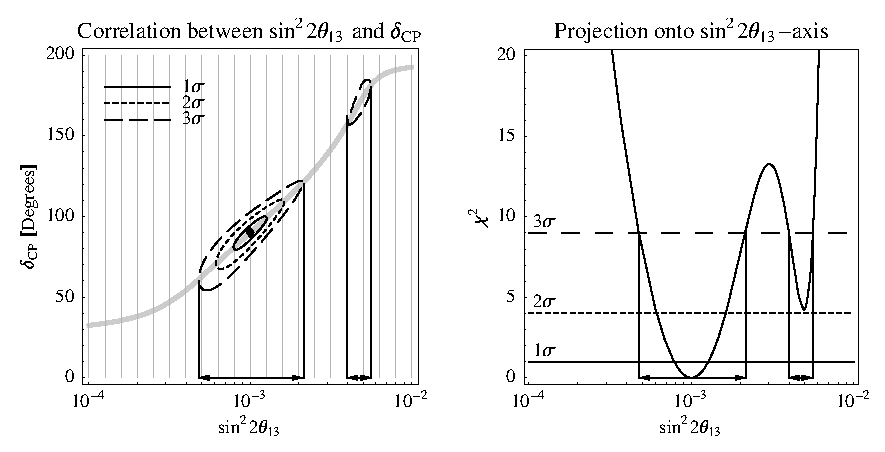
\includegraphics[width=16cm]{projex}
\end{center}
\mycaption{\label{fig:projex} Left plot: The correlation between $\stheta$ and $\deltacp$ as calculated in the example on page~\pageref{ex:corrth13dcp}, but for 1 d.o.f. only. Right plot: The $\chi^2$-value of the projection onto the $\stheta$-axis as function of $\stheta$. The projection onto the  $\stheta$-axis is obtained by finding the minimum $\chi^2$-value for each fixed value of $\stheta$ in the left-hand plot, \ie, along the gray vertical lines. The thick gray curve marks the position of these minima in the left-hand plot. The arrows mark the obtained fit ranges for $\stheta$ at the $3 \sigma$ confidence level (1 d.o.f.), \ie , the precision of $\stheta$.}
\end{figure}

The projection onto the $\stheta$- (or $\deltacp$-) axis is performed by fixing $\stheta$ (or $\deltacp$) and minimizing the $\chi^2$-function over all free fit parameters and the matter densities. We illustrate this method at the example of the projection of the two-dimensional manifold in the $\stheta$-$\deltacp$-plane onto the $\stheta$-axis in \figu{projex}. In this figure, the left-hand plot shows the correlation in the $\stheta$-$\deltacp$-plane computed with {\tt glbChiSys}. The right-hand plot illustrates the projection of this two-dimensional manifold onto the $\stheta$ axis by minimizing $\chi^2$ over $\deltacp$. In this simple example, the minimization is done along the vertical gray lines in the left hand plot. The obtained minima are located on the thick gray curve, which means the the right-hand plot represents the $\chi^2$-value along this curve. In fact, one can easily see that one obtains the correct projected $3 \sigma$ errors in this example (\cf, arrows). This figure illustrates the projection of a two-parameter correlation. In general, the full $n$-parameter correlation is treated similarly by the simultaneous (local) minimization over all free fit parameters. 

\index{Minimizer}
The following functions are some of the simplest minimizers 
provided by \GLOBES :
\begin{function}
\GLBNS{glbChiTheta}
{\tt double glbChiTheta(const glb\_params in, glb\_params out, int exp)}
returns the projected $\chi^2$ onto the $\theta_{13}$-axis for the  experiment {\tt exp}. For the simulation of all initialized experiments,
use {\tt GLB\_ALL} for {\tt exp}. The values in {\tt in} are the guessed fit values for the minimizer (all parameters other than $\theta_{13}$) and the fixed fit value of $\theta_{13}$. The actually determined parameters at the minimum are returned in {\tt out}, where $\theta_{13}$ is still at
its fixed value. If {\tt out} is set to {\tt NULL}, this information will not be returned.
\end{function}
\begin{function}
\GLBNS{glbChiDelta}
{\tt double glbChiDelta(const glb\_params in, glb\_params out, int exp)}
returns the projected $\chi^2$ onto the $\deltacp$-axis for the  experiment {\tt exp}. For the simulation of all initialized experiments,
use {\tt GLB\_ALL} for {\tt exp}. The values in {\tt in} are the guessed fit values for the minimizer (all parameters other than $\deltacp$) and the fixed fit value of $\deltacp$. The actually determined parameters at the minimum are returned in {\tt out}, where $\deltacp$ is still at its fixed value. If {\tt out} is set to {\tt NULL}, this information will not be returned.
\end{function}

All of the minimization functions have a similar parameter structure: The fixed fit parameter value and the guessed starting point of the minimizer, \ie, the guessed position of the minimum, are transferred in the list {\tt in}. Part of this list are the matter density
scaling factors of all experiments, which are also minimized over. 
The minimizer is then started at the guessed point and runs into
the local minimum, where the fit parameter of the projection
axis is fixed. For the best-fit solution, it is usually sufficient to start the minimizer at the best-fit point. However, the convergence speed might
be better by starting it slightly off this point. In addition, there
are problems in many cases with more complicated topologies, which means
that better guesses for the position of the minimum are needed.
The position of the minimum is then returned in {\tt out}
together with the number of iterations used for the minimization.
It is very often useful to print the output of the minimization with
\GLB{glbPrintParams} in order to check that the minimum is the
appropriate one. For example, if the minimizer ends up in the wrong-sign
solution in $\ldm$, priors can be used to force it into the tested
minimum. In addition, the number of iterations used allows an optimization
of the convergence speed. 
% 
Note that before any minimization, \GLB{glbSetStartingValues} 
and \GLB{glbSetInputErrors} have to be used at least once. In addition, note that the resulting $\chi^2$ of {\tt glbChiTheta} (or {\tt glbChiDelta}) for the combination of more than one experiment is not 
equal to the sum of the individual $\chi^2$-values anymore. This has two reasons: First, the topology of the fit manifold is altered by the addition of $\chi^2$-values of different experiments. Thus, after the minimization, the position of the minimum can be different to the ones of the individual experiments. Second, the priors for the external knowledge on the parameters are only added once -- independent of the number of experiments.

\index{Matter density scaling factor}
The the output of the minimizer in {\tt out} carries as many matter density scaling factors as there are experiments. Either
one (for the simulation of one experiment) or all (for the simulation of
all experiments) are different from $1.0$ if matter density uncertainties
are present, since each experiment may face other matter density conditions. The minimizer for individual experiments ``know'' which
experiment they are currently treating, which means that only the returned
matter density scaling factor of the appropriate experiment is modified.
For example, calculating {\tt glbChiTheta} for the last experiment
number, the last density values will be modified.
This approach turns out to be extremely useful together with the
simulation of more than one experiment. One can, for instance, locate the
degeneracies of all individual experiments. In order to test if
these degeneracies are still present in the combination of all experiments (which has a very different topology), one can test the combination of experiments with the output {\tt out} from the individual experiments. In this case, even the correct matter density scaling factor
output is used. 

The example on page~\pageref{ex:corrproj} demonstrates how one can obtain \figu{projex} (right) with keeping all parameters but $\deltacp$ fixed, as well as how one can include the full $n$-parameter correlation with external input. It also demonstrates how these two compare to each other. One can easily read off this example that 
there is a substantial impact of the
correlation with oscillation parameters other than $\deltacp$. 
Note that it uses the function
\GLB{glbChiNP} for arbitrary projections from the next section for the minimization over $\deltacp$.
In addition, there is one interesting feature in guessing the
oscillation parameters in this example: In order to avoid falling
into the wrong minimum, the fit value of $\deltacp$ is guessed from \figu{projex} (left). This quite sophisticated ``guessing'' is typical
for neutrino factories because of the $(\deltacp, \theta_{13})$-degeneracy, whereas it is for superbeams often sufficient
to use the best-fit values. A strong indication for a wrong guessing 
are discontinuous jumps in the projected $\chi^2$-function, where the minimizer jumps from one minimum to another. In such cases, the starting point of the minimizer has to be adjusted to help it find the true minimum.

Other examples for projections onto a parameter axis while keeping exactly one parameter fixed are \GLB{glbChiTheta23}, \GLB{glbChiDm}, and \GLB{glbChiDms}, which
can be found in \Tab~\ref{tab:stdfunctions} on page~\pageref{tab:stdfunctions}.

\section[Projection onto any hyperplane]{Projection onto any hyperplane}
\index{Projection onto hyperplane}

In general, one can show the measurement result in any $k$-dimensional hyperplane, where $k$ is smaller than the dimension of the parameter space $n$, and thus the dimension of the fit manifold. In this case, $k$ parameters are fixed and $n-k$ parameters are minimized over. One such example is the projection of the fit manifold onto the $\stheta$-$\deltacp$-plane, \ie, $k=2$ here. In this case, the two
parameters $\stheta$ and $\deltacp$ are kept fixed, and the others are
minimized over. 
The corresponding function is \index{Projection onto $\theta_{13}$-$\deltacp$-plane}
\begin{function}
\GLBNS{glbChiThetaDelta}
{\tt double glbChiThetaDelta(const glb\_params in, glb\_params out, int exp)} returns the projected $\chi^2$ onto the $\theta_{13}$-$\deltacp$-plane for the  experiment {\tt exp}. For the simulation of all initialized experiments,
use {\tt GLB\_ALL} for {\tt exp}. The values in {\tt in} are the guessed fit values for the minimizer (all parameters other than $\theta_{13}$ and $\deltacp$) and the fixed fit values of $\theta_{13}$ and $\deltacp$. The actually determined parameters at the minimum are returned in {\tt out}, where $\theta_{13}$ and $\deltacp$ are still at their fixed values. If {\tt out} is set to {\tt NULL}, this information will not be returned.
\end{function}
This function works analogously to the ones in the last section. They can, for example, be used to obtain a figure similar to \figu{projex}, left.
The example on page~\pageref{ex:corrproj} illustrates then the difference
between the projections of the ``eggs'' within the 
$\stheta$-$\deltacp$-plane onto the $\theta_{13}$-axis. 
Though the running time for one call of these functions is somewhat 
shorter than the one for the $\stheta$- or $\deltacp$-projections, one 
has to compute a two-dimensional array for such a figure (instead of a 
one-dimensional list). Therefore, the overall computational effort is 
much higher, \ie, in the order of hours. In many cases, it is therefore
convenient to run {\tt glbChiSys} first to obtain a picture of
the manifold and to adjust the parameter ranges. Then, one can run
{\tt glbChiThetaDelta} for a complete evaluation of the problem
including correlations.

\begin{table}[t!]
\begin{tabular}{p{4.2cm}p{5.5cm}p{5.1cm}}
\hline
Function & Purpose & Parameters $\rightarrow$ Result\\
\hline
\GLB{glbAllocProjection} & Create projection vector & {\tt ()} \\
\GLB{glbFreeProjection} & Destroy projection vector {\tt stale} & {\tt (glb\_projection stale)} \\
\GLB{glbDefineProjection} & Assign projection vector {\tt in} & {\tt (glb\_projection in, int theta12, int theta13, int theta23, int delta, int dms, int dma)} \\ 
\GLB{glbCopyProjection} & Copy vector {\tt source} to {\tt dest} & {\tt (const glb\_projection source, glb\_projection dest)} \\
\GLB{glbPrintProjection} & Print vector {\tt in} to file {\tt stream} & {\tt (FILE* stream, const glb\_projection in)} \\
\GLB{glbSetProjectionFlag} & Set flag for oscillation parameter {\tt which} in vector {\tt in} to value {\tt flag}. & {\tt (glb\_projection in, int flag, int which)} \\
\GLB{glbGetProjectionFlag} & Return flag for oscillation parameter {\tt which} in vector {\tt in}. & {\tt (const glb\_projection in, int which)} $\rightarrow$ {\tt int} flag \\
 {\tt glbSetDensity\-ProjectionFlag} \GLBNS{glbSetDensityProjectionFlag} & Set flag for density parameter {\tt which} in vector {\tt in} to value {\tt flag}. & {\tt (glb\_projection in, int flag, int which)} \\
{\tt glbGetDensity\-ProjectionFlag} \GLBNS{glbGetDensityProjectionFlag} & Return flag for density parameter {\tt which} in vector {\tt in}.  & {\tt (const glb\_projection in, int which)} $\rightarrow$ {\tt int} flag \\
\hline
\end{tabular}
\caption{\label{tab:defprojection}\index{Projection type}
Different functions handling the
\GLB{glb\_projection} type. Flags are either \GLB{GLB\_FIXED} or \GLB{GLB\_FREE}. The (un-shown) return values of the {\tt Set-} and {\tt Define-} functions point either to the assigned vector if successful, or they are {\tt NULL} if unsuccessful.}
\end{table}

In principle, one can also use three- or more-dimensional projections. In addition, one may want to use a different set of parameters for single- or two-parameter projections. The very flexible function \GLB{glbChiNP} is
designed for this purpose. However, because of its flexibility, it 
involves more sophistication.

In order to define arbitrary projections, we introduce the vector
\GLB{glb\_projection}, which is very similar to the
oscillation parameter vector {\tt glb\_params}.
Normally, the user does not need to access this type directly:
A set of function similar to the ones for {\tt glb\_params} is
provided. The purpose of {\tt glb\_projection} is to tell \GLOBES\ 
what parameters are fixed, and what are minimized over. Thus, in
comparison to {\tt glb\_params}, it does not take values for the
parameters, but flags \GLB{GLB\_FIXED} or \GLB{GLB\_FREE}.
For example, the projection onto the $\theta_{13}$-axis {\tt glbChiTheta}
is nothing else than a special case of {\tt glbChiNP} with $\theta_{13}$
fixed and all the other parameters free. Similar to {\tt glb\_params},
the type {\tt glb\_projection} has to be created first, and destroyed
later. The access functions for {\tt glb\_projection} are summarized in \Tab~\ref{tab:defprojection}. Since the complete set is very similar to
the one for {\tt glb\_params}, we do not go into greater details here.

\index{Projection: Define}
As soon as we have defined a projection, we can assign it:
\begin{function}
\GLBNS{glbSetProjection}
{\tt int glbSetProjection(const glb\_projection in)} sets the projection
to {\tt in}. The return value is $0$ if successful, and $-1$ if
unsuccessful.
\end{function}
Similarly, the currently assigned projection can be returned with:
\begin{function}
\GLBNS{glbGetProjection}
{\tt int glbGetProjection(glb\_projection out)} writes the currently
set projection to {\tt out}. The return value is $0$ if successful, and $-1$ if unsuccessful.
\end{function}
After setting the starting values, input errors, and the projection, 
we can run the minimizer:
\begin{function}
\GLBNS{glbChiNP}
{\tt double glbChiNP(const glb\_params in, glb\_params out, int exp)} 
returns the projected $\chi^2$ onto the hyperplane specified by 
{\tt glbSetProjection} for the  experiment {\tt exp}. 
For the simulation of all initialized experiments,
use {\tt GLB\_ALL} for {\tt exp}. The values in {\tt in} are the guessed fit values for the minimizer (all free parameters) and the fit values
on the hyperplane (all fixed parameters). The actually determined parameters at the minimum are returned in {\tt out}, where the fixed parameters are still at their input values. If {\tt out} is set to {\tt NULL}, this information will not be returned.
\end{function}
As an example, the projection sequence for a minimization over
$\deltacp$ only looks like this:
\begin{quote}
{\tt
  glb\_projection th13\_projection = glbAllocProjection(); \\
  glbDefineProjection(th13\_projection,GLB\_FIXED,GLB\_FIXED,GLB\_FIXED,\\
  \hspace*{2cm} GLB\_FREE,GLB\_FIXED,GLB\_FIXED); \\
  glbSetProjection(th13\_projection); \\ 
  res1=glbChiNP(test\_values,NULL,GLB\_ALL); \\
  glbFreeProjection(th13\_projection);
}
\end{quote}
In this case, only the correlation with $\deltacp$ is taken into account.
Note that in the  example on page~\pageref{ex:corrproj} this projection
is compared with the result including the full multi-parameter correlation.

\chapter{Locating degenerate solutions}
\index{Degenerate solutions}
\index{Degeneracies $\chi^2$}

In the last chapter, we introduced the projection of any set of $k$ parameter onto any $n-k$ dimensional hyperplane, which was done by the minimization over the $k$ free fit parameters. Similarly, one can minimize over {\em all} $n$ parameters to find the local minimum close to any starting point. This approach is very useful for the exact numerical location of a degeneracy if its approximate position is known. For the determination of the approximate position, one can use analytical approaches or an educated guess. 
Though the usage of the all-parameter minimizers is quite simple, one should keep in mind that they are local minimizers. Therefore, one may need a very sophisticated application software to find all degenerate solutions.

\example{Finding the $\mathrm{sgn}(\ldm)$-degeneracy}{
\label{ex:sgndeg}
\index{Degeneracies: sgn($\ldm$)-degeneracy}

In many cases, one can find the exact position of the $\mathrm{sgn}(\ldm)$-degeneracy with \GLB{glbChiAll}, where one starts 
the local minimizer at the suspected position 
and let it converge into the minimum.  The following code excerpt  corresponds to finding the degenerate solution for the example on
  page~\pageref{ex:corrth13dcp}, and it is from {\tt example3.c}: 
\begin{quote}
{\tt
{\footnotesize
  /* Set starting vales to suspected position at opposite sign of ldm */ \\
  \mbox{glbDefineParams(starting\_values,theta12,theta13,theta23,deltacp,sdm,-ldm);} \\
  \\
  /* Set input errors for external input, where some information on ldm \\
   \hspace*{0.5cm} is imposed in order to avoid falling into the right-sign solution */ \\
  glbDefineParams(input\_errors,theta12*0.1,0,0,0,sdm*0.1,ldm/3); \\ 
  glbSetDensityParams(input\_errors,0.05,GLB\_ALL); \\
  \\
  glbSetStartingValues(starting\_values); \\
  glbSetInputErrors(input\_errors); \\
  \\
  /* Localize degenerate solution by minimization over all parameters */ \\
  double CL=glbChiAll(starting\_values,deg\_pos,GLB\_ALL); \\
   \\
  \mbox{/* Now: CL is the chi2 of the deg.~solution and deg\_pos the position */} 
}}
\end{quote}

Using {\tt ent\_pos} to obtain a section of the degeneracy in the
$\stheta$-$\deltacp$-plane (\cf, {\tt example3.c}), one can plot it as a contour plot in addition to the original solution (2 d.o.f., gray curves):
\begin{center}
\colorbox{white}{\includegraphics[width=7.5cm]{correntex}}
\end{center}

}

\index{All-parameter minimization}
The function to perform the all-parameter minimization is {\tt glbChiAll}:
\begin{function}
\GLBNS{glbChiAll} 
{\tt double glbChiAll(const glb\_params in, glb\_params out, int exp)}
  returns the minimized $\chi^2$ over all parameters for the  experiment {\tt exp}. For the simulation of all initialized experiments,
use {\tt GLB\_ALL} for {\tt exp}. The values in {\tt in} are the guessed fit values for the minimizer. The actually determined parameters at the minimum are returned in {\tt out}. If {\tt out} is set to {\tt NULL}, this information will not be returned.
\end{function}
%
This function takes the suspected position of the local minimum and returns its actual position in {\tt out}, as well as the $\chi^2$-value 
at the minimum as return value. Thus, the return value can be immediately
used to judge whether the located degeneracy appears at the chosen
confidence level.

The example on page~\pageref{ex:sgndeg} illustrates how to locate the $\mathrm{sgn}(\ldm)$-degeneracy and show the corresponding degenerate solution in the $\stheta$-$\deltacp$-plane together with the original solution.
In this case, the position of the degeneracy can be easily guessed to be at the best-fit parameter values but the $\ldm$ inverted. The minimizer then runs off the plane of the best-fit parameters into the local minimum. It is very important to take into account the position of the degeneracy off this plane, since the actual $\chi^2$ in the minimum is certainly lower than on the plane of the best-fit parameter values. Thus, the degeneracy may not even appear at the chosen confidence level on the plane, but it does appear at the true minimum. The two sections\footnote{The discussed figure on page~\pageref{ex:sgndeg} is produced by  {\tt glbChiSys} and thus only represents a section through the fit manifold. For the projection including correlations, one may rather want to use {\tt glbChiThetaDelta}.} through the fit manifold shown in the figure on page~\pageref{ex:sgndeg} therefore do not appear at the same oscillation parameter values (except from the ones shown in the figure). 

\index{Advanced tricks}
For the more advanced reader, a number of tricks can be useful for the numerical localization of degenerate solutions:
\begin{description}
\item[Minimum $\boldsymbol{\chi^2}$ larger than threshold.] If a located degeneracy has a minimum $\chi^2$ larger than the corresponding confidence level threshold for the discussed quantity of interest, the degeneracy can be immediately ignored. This saves a lot of computation time.
\item[Locating degeneracies in more complicated topologies.] For more complicated topologies, such as for neutrino factories, it is often useful to use multi-step location procedures or analytical knowledge. For example, for a numerical procedure, one may first of all switch off the systematics and keep $\stheta$ or $\deltacp$ fixed, \ie, use {\tt glbChiTheta}, where $\stheta$ or $\deltacp$ is fixed at the best-fit value. The result can then be used as a starting point for {\tt glbChiAll} for the individual experiments with the systematics switched on again. 
\item[Forcing the minimizer into the targeted solution.]
In addition to switching off the systematics, it can be useful to reduce the input errors during some steps of the localization process in order to make the minimizer not to run away too much from the targeted solution.
The example on page~\pageref{ex:sgndeg} illustrates this with the
input error for $\ldm$: Since the guessed starting point might be
quite far away from the real degeneracy, the algorithm may in some cases
find the original solution instead of the degeneracy (which can
be immediately seen from the output vector). The input error
for $\ldm$ gives the algorithm a ``bias'' against the original solution.
However, note that the input error must not be too small in order
to avoid a significant contribution of the prior to the final $\chi^2$.
Alternatively, one could run {\tt glbChiAll} again with the located minimum
as {\tt in} vector and $\ldm$ kept free.
\item[Finding degeneracies with multiple experiments.] For multiple experiments, it turns out to be useful to locate the degeneracies for individual experiments first. Then, all of the found degeneracies below the threshold can be tested for the combination of all experiments.
\end{description}
Finally, note that any degenerate solution below the confidence level threshold which can not be located makes the result appear better than it actually is. Thus, one should be careful with the determination of the degenerate solutions in order to find all of them.

\chapter{Obtaining low-level information}
\index{Low-level information}

In this chapter, we discuss possibilities to obtain low-level information
in \GLOBES , \ie, about oscillation probabilities, rates, and other
information lower than on the $\chi^2$-level.

\section{Oscillation probabilities}
\index{Oscillation probabilities}

\GLOBES\ can compute the probabilities in vacuum
with the following function:
\begin{function}
\GLBNS{glbVacuumProbability}
{\tt double glbVacuumProbability(int l, int m, int panti,double E, double L)} returns the neutrino oscillation probability $\nu_l \rightarrow \nu_m$ for the energy {\tt E} and the baseline {\tt L} in vacuum. The parameter
{\tt panti} is $+1$ for neutrinos and $-1$ for antineutrinos. 
\end{function}
In addition, the oscillation probabilities in matter can be obtained
with:
\begin{function}
\GLBNS{glbProfileProbability}
{\tt double glbProfileProbability(int l, int m, int panti,double E)}
 returns the neutrino oscillation probability $\nu_l \rightarrow \nu_m$ for the energy {\tt E} in matter. The parameter
{\tt panti} is $+1$ for neutrinos and $-1$ for antineutrinos.
The matter density profile including baseline is the one from the last
evaluated experiment. 
\end{function}
THIS FUNCTION MAY OBTAIN AN EXPERIMENT INDEX (WW).
\section{Event rates}
\index{Event rates}
One can also return event rates in \GLOBES , but this feature
requires some knowledge about the experiment definition. 
In fact, many of these functions are very advanced, which means
that the reader who wants to use them should be familiar with
\Secs~\ref{sec:channel} and~\Sec~\ref{sec:rules} of the \AEDL\ manual.

\index{Event rates}
\GLOBES\ currently supports rule-based and channel-based event rate functions, where the information is in written into a file
or returned in a list. The rule-based functions are:
\begin{function}
\GLBNS{glbShowRuleRates}
{\tt int glbShowRuleRates(FILE* stream, int exp, int rule, int pos,
int effi, int bgi, int coeffi, int signal)} prints the binned rule rates as
list with energy and event rate to the file {\tt stream} (either an
open file, or {\tt stdout}). A specific experiment {\tt exp} and a 
specific rule {\tt rule} have to be chosen, as well as the signal
or background rate {\tt signal} (either \GLB{GLB\_SIG} or \GLB{GLB\_BG}).
The position {\tt pos} refers to the component within the signal or 
background, and can also be {\tt GLB\_ALL}. The function may return
the rates with (\GLB{GLB\_W\_COEFF}) or without (\GLB{GLB\_WO\_COEFF})
overall efficiency coefficient, as it is specified by {\tt coeffi}. 
In addition, it may contain the post-smearing efficiencies (set
{\tt effi} to \GLB{GLB\_W\_EFF} or \GLB{GLB\_WO\_EFF}), and the
post-smearing backgrounds (set
{\tt bgi} to \GLB{GLB\_W\_BG} or \GLB{GLB\_WO\_BG}). The pre-smearing
efficiencies and backgrounds cannot be accessed at the rule level.
The return value
is $0$ if successful, and $-1$ if unsuccessful.
\end{function}
\begin{function}
\GLBNS{glbTotalRuleRate}
{\tt double glbTotalRuleRate(int exp, int rule, int pos,
int effi, int bgi, int coeffi, int signal)} returns the total rates with
the same parameters as {\tt glbShowRuleRates}.
\end{function}
The function {\tt glbTotalRuleRate} is especially useful if
one wants to draw bi-rate graphs with total event rates, or look
for the $(\deltacp,\theta_{13})$-degeneracy by the intersection of 
neutrino and antineutrino constant event rate curves.
%
In order to obtain information on the structure of the rules, 
a number of additional functions are provided:
\begin{function}
\GLBNS{glbGetNumberOfRules}
{\tt int glbGetNumberOfRules(int exp)} returns the number of
rules in experiment {\tt exp}.
\end{function}
\begin{function}
\GLBNS{glbGetLengthOfRule}
{\tt int glbGetLengthOfRule(int exp, int rule, int signal)} returns
the length of rule {\tt rule} in experiment {\tt exp}. The parameter
{\tt signal} can be either \GLB{GLB\_SIG} for the number of signal
components or \GLB{GLB\_BG} for the number of background components.
\end{function}
\begin{function}
\GLBNS{glbGetNormalizationInRule}
{\tt double glbGetNormalizationInRule(int exp, int rule, int signal)}
returns the normalization (normalization or background center)
in rule {\tt rule} of the experiment {\tt exp}.
The parameter {\tt signal} refers to signal (\GLB{GLB\_SIG}) or background
(\GLB{GLB\_BG}).
\end{function}
\begin{function}
\GLBNS{glbGetChannelInRule}
{\tt int glbGetChannelInRule(int exp, int rule, int pos, int signal)}
returns the channel number in rule {\tt rule} at the position {\tt pos}
of the experiment {\tt exp}.
The parameter {\tt signal} refers to signal (\GLB{GLB\_SIG}) or background
(\GLB{GLB\_BG}).
\end{function}
\begin{function}
\GLBNS{glbGetCoefficientInRule}
{\tt double glbGetCoefficientInRule(int exp, int rule, int pos, int signal)}
returns the coefficient of the component {\tt pos} in rule {\tt rule} 
of the experiment {\tt exp}.
The parameter {\tt signal} refers to signal (\GLB{GLB\_SIG}) or background
(\GLB{GLB\_BG}).
\end{function}


In addition, \GLOBES\ has channel-based rate functions:
\begin{function}
\GLBNS{glbShowChannelRates}
{\tt int glbShowChannelRates(FILE *stream,
int exp, int channel, int smearing, int effi, int bgi)}
prints the binned channel rates as
list with energy and event rate to the file {\tt stream} (either an
open file, or {\tt stdout}). A specific experiment {\tt exp} and a 
specific channel {\tt channel} have to be chosen.
The function may return
the rates before (\GLB{GLB\_PRE}) or after (\GLB{GLB\_POST})
the energy smearing, as it is specified by {\tt smearing}.
In addition, it may contain the pre- and post-smearing efficiencies (set
{\tt effi} to \GLB{GLB\_W\_EFF} or \GLB{GLB\_WO\_EFF}), and the
pre- and post-smearing backgrounds (set
{\tt bgi} to \GLB{GLB\_W\_BG} or \GLB{GLB\_WO\_BG}). Note that
the post-smearing efficiencies and backgrounds cannot be taken into
account if the rates are returned before the energy smearing.
The return value
is $0$ if successful, and $-1$ if unsuccessful.
\end{function}
\begin{function}
\GLBNS{glbGetChannelRates}
{\tt int glbGetChannelRates(double** data,
size\_t* length, int exp, int channel, int smearing)}
writes the binned raw channel rates to the list {\tt data}
and the length of this list to {\tt length}. 
A specific experiment {\tt exp} and a 
specific channel {\tt channel} have to be chosen.
The function may return
the rates before ({\tt smearing} is \GLB{GLB\_PRE}) or after ({\tt smearing} is \GLB{GLB\_POST})
the energy smearing, where no user-defined data
(pre-/post-smearing efficiencies or backgrounds) are taken into account.
The return value is $-1$ if unsuccessful.
\end{function}
\begin{function}
\GLBNS{glbGetUserData}
{\tt int glbGetUserData(double** data,
size\_t* length, int exp, int channel, int smearing, int bgeff)}
writes the binned user-defined backgrounds or efficiencies 
to the list {\tt data} and the length of this list to {\tt length}. 
A specific experiment {\tt exp} and a 
specific channel {\tt channel} have to be chosen.
The function may return
the pre- ({\tt smearing} is \GLB{GLB\_PRE}) or post- ({\tt smearing} is \GLB{GLB\_POST}) smearing backgrounds ({\tt bgeff} is \GLB{GLB\_BG}) 
or efficiencies ({\tt bgeff} is \GLB{GLB\_EFF}). 
The return value is $-1$ if unsuccessful.
\end{function}
Since \GLOBES\ reserved the memory for the lists returned in these
functions, which it allocates on an internal stack, one has to reset
the stack at the end of the rates access with
\begin{function}
\GLBNS{glbResetRateStack}
{\tt void glbResetRateStack()} resets the rate stack used for the
lists returned from {\tt glbGetChannelRates} or {\tt glbGetUserData}.
\end{function}
A code excerpt to show the channel rates may look like this:
\begin{quote}
{\tt
 double* rates; \\
  size\_t length; \\
  glbGetChannelRates(\&rates,\&length,0,0,GLB\_PRE); \\
  int i; \\
  for(i=0;i<length;i++) printf("\%g $\backslash$n",rates[i]); \\
  glbResetRateStack(); \\
}
\end{quote}
Finally, one can find the number of channels of an experiment:
\begin{function}
\GLBNS{glbGetNumberOfChannels}
{\tt int glbGetNumberOfChannels(int exp)} returns the number of 
channels of experiment {\tt exp}.
\end{function}

\section{Fluxes and cross sections}
\index{Flux} \index{Cross section}

Another piece of low-level information, which can be returned by \GLOBES ,
are the numbers from the loaded fluxes and cross sections.
The following functions interpolate on the loaded fluxes and cross 
sections, \ie, any value in the allowed energy range can be given as input:
\begin{function}
\GLBNS{glbFlux}
{\tt double glbFlux(int exp, int ident, 
double E, double distance, int l, int anti)} returns
the flux of flux number {\tt ident} of the experiment {\tt exp}
for the flavor $\nu_l$ 
and polarity {\tt anti} ($+1$: neutrinos, $-1$: antineutrinos) at the energy {\tt E} and distance {\tt distance}.
\end{function}

\begin{function}
\GLBNS{glbXSection}
{\tt double glbXSection(int exp, 
int ident, double E, int l, int anti)} returns
the cross section of experiment {\tt exp}, 
cross section number {\tt ident} for the flavor $\nu_l$ and polarity {\tt anti} ($+1$: neutrinos, $-1$: antineutinos) at the energy {\tt E}.
\end{function}
Note that all flux or flavor numbers run from $0$ to $N-1$ in these functions.

\chapter{Changing experiment parameters at running time}
\label{chapt:running}
\index{Experiment parameters}

Many of the parameters in experiment definitions can be changed
at running time. For example, we have introduced in 
\Sec~\ref{sec:luminosity} possibilities to change the integrated
luminosity, which consists of source power, running time, and target mass.
In this chapter, we discuss more sophisticated
experiment changes. However, since \GLOBES\ computes a lot of
information only once when an experiment is loaded, many
parameters can not be changed at running time. For example,
the energy resolution function or the number of bins are used
to compute the smearing matrix already at the initialization
of the experiment, which saves a lot of computation
time for most applications. In \Sec~\ref{sec:aedlparams}, we 
introduce a mechanism how one can even change these \AEDL\ parameters
during running time.

\section{Baseline and matter density profile}
\index{Baseline: Change}
\index{Matter density profile: Change}

In order to change the baseline of an experiment, it is important
to keep in mind that each experiment has a profile type defined
in the \AEDL\ file (average density, PREM profile with a given
number of steps, or arbitrary profile). One can check the currently
used profile type with
\begin{function}
\GLBNS{glbGetProfileType}
{\tt int glbGetProfileType(int exp)} returns the matter density profile
type of experiment {\tt exp}.
\end{function}
For each profile type, one can easily change the baseline with {\tt glbSetBaselineInExperiment},
where the average density or the PREM profile are re-computed, or the
steps in the arbitrary profile are re-scaled. Of course, though this
function is sufficient in most cases, it does often not make sense
for arbitrary matter density profiles.
\begin{function}
\GLBNS{glbSetBaselineInExperiment}
{\tt int glbSetBaselineInExperiment(int exp, double baseline)}
sets the baseline length in experiment {\tt exp} to {\tt baseline}.
The function returns $-1$ if it was not successful.
\end{function}
Note that {\tt glbSetBaselineInExperiment} does not change the
profile type in the experiment. The counterpart of this function is:
\begin{function}
\GLBNS{glbGetBaselineInExperiment} 
{\tt double glbGetBaselineInExperiment(int exp)} returns the
baseline length currently used for experiment {\tt exp}.
\end{function}
One can not change the profile type of an experiment manually
during running time. However, one can change the matter density
profile, where the profile type is automatically changed to three
(arbitrary matter density profile). In addition, a number of functions 
are provided to compute possible matter density profiles (average density,
PREM profile). In general, a matter density profile in \GLOBES\ with
$N$ layers is represented by a list of lengths 
\begin{equation}
\mathrm{Lengths} = (x_1,x_2, \hdots, x_N) 
\end{equation}
and a list of densities
\begin{equation}
\mathrm{Densities} = (\rho_1,\rho_2, \hdots, \rho_N), 
\end{equation}
where the baseline is given by
\begin{equation}
L = \sum\limits_{i=1}^N x_i.
\end{equation}
In C, lists are represented as pointers to the first element:
\begin{quote}
{\tt  
  double* lengths; \\
  double* densities;
}
\end{quote}
Many of the \GLOBES\ baseline functions take and return
such lists as parameters, and are therefore more sophisticated
to handle. In general, any function
{\em returning} lists reserves the memory space for them.
It is then up to the user to return the allocated memory!
In addition, they normally return the length of the lists $N$
in form of a pointer, where the corresponding memory space 
has to be provided by the user (normally, it is enough to declare
a variable of the type {\tt size\_t} corresponding to positive
integer numbers).
The following functions return matter density profiles:
\begin{function}
\GLBNS{glbLoadProfileData}
{\tt int glbLoadProfileData(const char* filename, size\_t *layers, double **lengths, double **densities)} loads a density file from the file
{\tt filename}. It returns the number of layers {\tt layers}, the
list of lengths {\tt lengths}, and the list of densities {\tt densities}.
\end{function}
The file should contain in each line a length and density for one layer,
which are separated by an empty space.
\begin{function}
\GLBNS{glbStaceyProfile}
{\tt int glbStaceyProfile(double baseline, size\_t layers, double **lengths, double **densities)} creates a PREM/Stacey matter density profile with a
number of {\tt layers} steps for the baseline {\tt baseline}. The list of lengths {\tt lengths} and the list of densities {\tt densities} are returned.
\end{function}
\begin{function}
\GLBNS{glbAverageDensityProfile}
{\tt glbAverageDensityProfile(double baseline, double **lengths, 
double **densities)} creates a average matter density profile from the PREM/Stacey profile with one step for the baseline {\tt baseline}. The list of lengths {\tt lengths} and the list of densities {\tt densities} are returned.
\end{function}
\begin{function}
\GLBNS{glbStaceyProfile}
{\tt int glbGetProfileDataInExperiment(int exp,size\_t *layers, double** lengths, double** densities)} returns the matter density profile 
currently used for experiment {\tt exp}. The number of layers {\tt layers}, the list of lengths {\tt lengths}, and the list of densities {\tt densities} are returned.
\end{function}
All these functions return $-1$ if they were not successful.

The counterpart of these functions to assign a specific matter density
profile to an experiment is
\begin{function}
\GLBNS{glbSetProfileDataInExperiment}
{\tt int glbSetProfileDataInExperiment(int exp, size\_t layers,const double* lengths, const double* densities)} sets the matter density of experiment
{\tt exp} to an arbitrary profile with {\tt layers} steps. The density
layers are specified by the lists {\tt lengths} and {\tt densities}.
The function returns $-1$ if it was not successful.
\end{function}
Note that this function requires that the memory space for the lists
be reserved already.

Finally, let us take a look at two examples. This example changes
the baseline length to $7\,500 \, \mathrm{km}$, where the average 
matter density is manually computed:
\begin{quote}
{\tt  
  double* lengths; \\
  double* densities; \\
  glbAverageDensityProfile(7500,\&lengths,\&densities); \\
  glbSetProfileDataInExperiment(0,1,lengths,densities); \\
  free(lengths); \\
  free(densities); \\
}
\end{quote}
In the second example, we change the baseline to a PREM profile with
$100$ matter density steps and print them:
\begin{quote}
{\tt
  double* lengths; \\
  double* densities; \\
  glbStaceyProfile(7500,100,\&lengths,\&densities); \\
  int i; \\
  for(i=0;i<100;i++) printf("\%g \%g $\backslash$n",lengths[i],densities[i]); \\
  glbSetProfileDataInExperiment(0,100,lengths,densities); \\
  free(lengths);\\
  free(densities);\\
}
\end{quote}

\example{The impact of systematics, correlations, and degeneracies}{
\label{ex:barcharts}
\index{Bar charts}
\index{Systematics on/off}
Here it is demonstrated how one can successively include systematics, correlations, and degeneracies at the example of the $\stheta$-sensitivity limit.
An important part of this example is how two switch the systematics off,
\ie, how to obtain the sensitivity limit from statistics only. Since
this example is very advanced, we only show the respective function of the code:
\begin{quote}
{\tt 
/* Calculate chi2 with statistics only */ \\
double CalcNoSystematics(double theldm,double thex) \\
\{ \\
\hspace*{0.5cm} /* Switch systematics off for all exps and all rules */ \\
\hspace*{0.5cm} glbSwitchSystematics(GLB\_ALL,GLB\_ALL,GLB\_OFF); \\
\\
\hspace*{0.5cm} /* Calculate Chi2-list as if systematics were on */ \\
\hspace*{0.5cm} double res=CalcSystematics(theldm,thex); \\
\\
\hspace*{0.5cm} /* Switch systematics on for all exps and all rules */ \\
\hspace*{0.5cm} glbSwitchSystematics(GLB\_ALL,GLB\_ALL,GLB\_ON); \\
\\
\hspace*{0.5cm} return res; \\
\} \\
}
\end{quote}

\vspace*{-0.5cm}

The complete code can be found as {\tt example4.c} with the software,
which consists of many of the applications from the earlier examples.
In addition, it uses a little trick: It avoids falling into the wrong
 solution with {\tt glbChiTheta}
by using the fit value of $\deltacp$ from the step before as prediction
of the position of the current calculation.

The returned lists of data from the example represent $\chi^2$ 
as function of the fit value of $\stheta$. The intersections of these
curves with the line $\chi^2 = 9$ give the $\stheta$ sensitivity
limits at the $3 \sigma$ confidence level, where we do not include the
 $\mathrm{sgn}(\ldm)$- and $(\deltacp,\theta_{13})$-degeneracies in the sensitivity limit with correlations only (green bar):
\begin{center}
\colorbox{white}{\includegraphics[width=6.5cm]{barsex}}
\end{center}
}

\section{Systematics}
\index{Systematics}
\index{Systematics on/off}

Changing the systematics at running time can be useful to investigate
the impact factors affecting the measurement.
In \GLOBES , the systematics is defined rule-based, \ie, each rule
has its own systematics. In addition, \AEDL\ requires that it has to be
defined in each rule what ``Systematics on'' and ``Systematics off'' means.
Therefore, it is usually very simple to switch the systematics on and off:
\begin{function}
\GLBNS{glbSwitchSystematics}
{\tt int glbSwitchSystematics(int exp, int rule, int on\_off)}
switches the systematics in experiment {\tt exp} and rule {\tt rule}
on ({\tt on\_off} is \GLB{GLB\_ON}) or off ({\tt on\_off} is \GLB{GLB\_OFF}). For the experiment or
rule index, one can also use \GLB{GLB\_ALL}. 
\end{function}
In the example on page~\pageref{ex:barcharts}, the application of
{\tt glbSwitchSystematics} is demonstrated to show the impact of
systematics, correlations, and degeneracies.

\index{Error dimension}
The error dimension (for the definition, see \Sec~\ref{sec:rules}) can also be accessed directly with 
\begin{function}
\GLBNS{glbSetErrorDim}
{\tt int glbSetErrorDim(int exp, int rule, int on\_off, int value)}
sets the error dimension for systematics on ({\tt on\_off} is \GLB{GLB\_ON}) or off ({\tt on\_off} is \GLB{GLB\_OFF}) of experiment {\tt exp} and rule {\tt rule} to the value {\tt value}. The function returns
$-1$ if not successful.
\end{function}
\begin{function}
\GLBNS{glbGetErrorDim}
{\tt int glbGetErrorDim(int exp, int rule, int on\_off)}
returns the error dimension for systematics on ({\tt on\_off} is \GLB{GLB\_ON}) or off ({\tt on\_off} is \GLB{GLB\_OFF}) of experiment {\tt exp} and rule {\tt rule}.
\end{function}

\index{Signal errors}
\index{Background errors}
\index{Background centers}
Except from the general treatment of systematics, one can read out
and write the signal and background errors, as well as the background
centers. For the definitions of these quantities, see \Sec~\ref{sec:rules}.
\begin{function}
\GLBNS{glbSetSignalErrors}
{\tt int glbSetSignalErrors(int exp, int rule, double norm, double tilt)}
sets the signal errors of experiment {\tt exp} and rule {\tt rule}
to {\tt norm} (normalization error) and {\tt tilt} (tilt/calibration error).
\end{function}
\begin{function}
\GLBNS{glbGetSignalErrors}
{\tt int glbGetSignalErrors(int exp, int rule, double* norm, double* tilt)}
writes the signal errors of experiment {\tt exp} and rule {\tt rule}
to {\tt norm} (normalization error) and {\tt tilt} (tilt/calibration error).
\end{function}
\begin{function}
\GLBNS{glbSetBGErrors}
{\tt int glbSetBGErrors(int exp, int rule, double norm, double tilt)}
sets the background errors of experiment {\tt exp} and rule {\tt rule}
to {\tt norm} (normalization error) and {\tt tilt} (tilt/calibration error).
\end{function}
\begin{function}
\GLBNS{glbGetBGErrors}
{\tt int glbGetBGErrors(int exp, int rule, double* norm, double* tilt)}
writes the background errors of experiment {\tt exp} and rule {\tt rule}
to {\tt norm} (normalization error) and {\tt tilt} (tilt/calibration error).
\end{function}
\begin{function}
\GLBNS{glbSetBGCenters}
{\tt int glbSetBGCenters(int exp, int rule, double norm, double tilt)}
sets the background centers of experiment {\tt exp} and rule {\tt rule}
to {\tt norm} (normalization center) and {\tt tilt} (tilt/calibration center).
\end{function}
\begin{function}
\GLBNS{glbGetBGCenters}
{\tt int glbGetBGCenters(int exp, int rule, double* norm, double* tilt)}
writes the background centers of experiment {\tt exp} and rule {\tt rule}
to {\tt norm} (normalization center) and {\tt tilt} (tilt/calibration center).
\end{function}
As usual, all these functions return $-1$ if they were not successful.

\section{External parameters in \AEDL\ files}
\label{sec:aedlparams}
\index{External \AEDL\ parameters}

Using external parameters in \AEDL\ files is a very powerful feature
to change experiment parameters at running time which require that
the experiment be re-initialized. For example, one can change the
energy resolution function or the number of energy bins. However,
in some cases there might be complications, such that the number
of pre- or post-smearing efficiencies does not correspond to the number
of energy bins anymore. Therefore, this feature needs to be 
used with care.

In order to use external parameters in \AEDL\ files, one simply
introduces them. For example, an energy resolution function
\begin{quote}
{\tt
energy(\#EnergyResolution1)< \\
\hspace*{1cm} type = 1 \\
\hspace*{1cm} @sigma\_e = \{ myres ,0,0 \} \\
> \\
}
\end{quote}
might be defined in \AEDL , where the energy resolution is proportional
to {\tt myres} $\times$ energy. 

In order to use the user-defined variable, one has to assign it 
with {\tt glbDefineAEDLVariable} {\em before} the experiment is initialized with \GLB{glbInitExperiment}:
\begin{function}
\GLBNS{glbDefineAEDLVariable}
{\tt void glbDefineAEDLVariable(const char* name, double value)}
assigns the value {\tt value} to the \AEDL\ variable {\tt name}.
\end{function}
In our energy resolution example, one could now loop over the
energy resolution such as with
\begin{quote}
{\tt
int i; \\
for(i=5;i<20;i++) \\
\{ \\    
\hspace*{1cm} glbClearExperimentList(); \\
\hspace*{1cm} glbDefineAEDLVariable("myres",0.01*i); \\
\hspace*{1cm} glbInitExperiment(...); \\
\\
\hspace*{1cm} /* do something */ \\
\}
}
\end{quote}
Note that one does not have do re-initialize the oscillation
parameter vectors every time within the loop as long as the
number of experiments does not change.

In order to clear the external variable stack if one is
excessively using it, one can use
\begin{function}
\GLBNS{glbClearAEDLVariables}
{\tt void glbClearAEDLVariables()}
clears the \AEDL\ variable list.
\end{function}
This function is called automatically upon exit of the program.

\section{Algorithm parameters: Filter functions}
\index{Filter functions}

The oscillation frequency filters to filter fast oscillations
can also be accessed by the user interface. For details of
the filter functions, we refer to \Sec~\ref{sec:energy} of
the \AEDL\ manual.

In particular, there are a number of functions:
\begin{function}
\GLBNS{glbSetFilterState}
{\tt int glbSetFilterState(int on\_off)} sets the filter state to
on (\GLB{GLB\_ON}) or off (\GLB{GLB\_OFF}).
\end{function}
\begin{function}
\GLBNS{glbGetFilterState}
{\tt int glbGetFilterState()} returns the filter state.
\end{function}
\begin{function}
\GLBNS{glbSetFilterStateInExperiment}
{\tt int glbSetFilterStateInExperiment(int exp, int on\_off)} sets the filter state in experiment {\tt exp} to on (\GLB{GLB\_ON}) or off (\GLB{GLB\_OFF}).
\end{function}
\begin{function}
\GLBNS{glbGetFilterStateInExperiment}
{\tt int glbGetFilterStateInExperiment(int exp)} returns the filter state of experiment {\tt exp}.
\end{function}
Analogously, the filter value can be accessed:
\begin{function}
\GLBNS{glbSetFilter}
{\tt int glbSetFilter(double filter)} sets the filter to the
value {\tt filter}.
\end{function}
\begin{function}
\GLBNS{glbGetFilter}
{\tt double glbGetFilter()} returns the filter value.
\end{function}
\begin{function}
\GLBNS{glbSetFilterInExperiment}
{\tt int glbSetFilterInExperiment(int exp, double filter)} sets the filter  in experiment {\tt exp} to the value {\tt value}.
\end{function}
\begin{function}
\GLBNS{glbGetFilterInExperiment}
{\tt double glbGetFilterInExperiment(int exp)} returns the filter value of experiment {\tt exp}.
\end{function}
The return value of all {\tt Set-} functions is $-1$ if they were not successful.


%%%%%%%%%%%%%%%%%%%%%%%%%%%%%%%%%%%
% PART II: Experiment definition module
%%%%%%%%%%%%%%%%%%%%%%%%%%%%%%%%%%%

%%%%%%%%%%%%%%%%%%%%%%%%%%%%%%%%%%%
% PART II: Experiment definition module
%%%%%%%%%%%%%%%%%%%%%%%%%%%%%%%%%%%

\part{The Abstract Experiment Definition Language -- AEDL}

\chapter{Getting started}

Here the general concept of the AEDL is described and illustrated by an example. In addition, a short introduction to the syntax of the AEDL is given.

\section{General concept of the experiment simulation}

The goal of AEDL is to describe a large number of complex and very 
different experiments by a limited number of parameters. It allows a
representation of very different setups within one data structure, and thus implements universal rate and $\chi^2$ computation methods. For experiment simulations, a new piece of code is usually written and compiled
for each different experiment. In many cases, even parameter changes, such as
the number of bins, requires the recompilation of the source code. 
However, such a technique soon reaches its limits when the simulated experiments are rather complex, or more than one type of experiment is studied simultaneously. Furthermore, it is very difficult to verify the correctness of the obtained results, since every time a new piece of code is added to 
deal with a new experiment type, new errors will be introduced.

Thus, a general and flexible experiment description language is needed.  
The description of a neutrino experiment can be split into three parts: Source, oscillation, and detection. The neutrino sources within \GLOBES\ 
are assumed to be stationary point sources, where each experiment has only 
one source. This restricts the classes of neutrino sources which can be studied with \GLOBES :
\begin{itemize}
\item
 Experiments using many point-like sources can only be approximated. One example are reactor experiments using many distant reactor blocks.
\item
 Geometrical effects of a source distribution, such as in the sun or the atmosphere, can not be described.
\item
 Sources with a physically significant time dependencies  can not be studied, such as  supernov\ae. It is, however, possible
to study beams with bunch structure, since the time dependence of the
neutrino source is physically only important to suppress backgrounds. 
\end{itemize}

The description of the neutrino oscillation physics is, at least numerically, relatively simple. We use the {\em evolution operator method} to compute the neutrino oscillation probabilities and divide the matter density profile into layers with constant matter densities. For each of these layers, the Hamiltonian in matter is diagonalized in order to propagate the neutrino transition amplitudes. Finally, the transition probability is obtained by the absolute square of the total neutrino transition amplitudes. Depending on the precision of the studied experiment, this approach turns out to be precise enough in Earth matter even for a small number matter density steps. Since we allow an uncertainty of the matter density profile, it is, in fact, in most cases sufficient to consider only one density step with the average matter density together with a matter density uncertainty~\cite{Ohlsson:2003ip}. Note that this approach may not be applicable to quickly varying extraterrestrial matter density profiles.

While it is comparatively simple to define a general neutrino source 
and to compute the oscillation physics, the general properties of a detector simulation are much more complicated. The basic assumption in building an abstract detector description is \emph{linearity}, \ie , that two neutrino events do not interfere with each other. Furthermore it is assumed that all information on the oscillation physics 
is given by the \emph{reconstructed} flavor and energy of a 
neutrino event. The term ``reconstructed'' implies that the well-defined energy of the incident neutrino, which can not be directly observed, translates via secondary particles and the detection properties into a distribution of possible energy values. This process is illustrated in \figu{distro} for the energy variable. 
%
\begin{figure}[ht]
\begin{center}
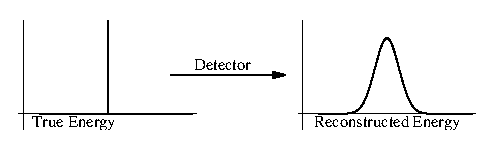
\includegraphics[width=0.6\textwidth]{mapping}
\end{center}
\caption{\label{fig:distro} A detector maps a true parameter value onto
a distribution of reconstructed parameter values. This is illustrated here for there energy.}
\end{figure}
% 
The same, in principle, applies to the nature of the neutrino flavor. However, in this case only discrete values are applicable. Note that the reconstructed neutrino energy and the neutrino flavor are the only observables in \GLOBES .

This picture can also be formulated in a more mathematical way. Let us define $x$ as the true parameter value and $x'$ as the reconstructed parameter value. Similarly, $f(x)$ is the distribution of true parameters values and $p(x')$ is the distribution of reconstructed parameter values. Then the detector function  $D(x,x')$, which describes the mapping performed by the detector, is given by
\begin{eqnarray}
\label{equ:mapping}
p(x')&=&\int dx\, f(x)\cdot D(x,x')\,.
\end{eqnarray}
Obviously \equ{mapping} only describes the detector properly
if the linearity condition is fulfilled. Within this model, a detector
is completely specified by a set of $D(E,E')$ for the energy variable $E$,
and a set $D(F,F')$ for the flavor variable $F$. In general, $D(E,E')$ also depends on the true flavor $F$, as well as $D(F,F')$ depends on the true energy $E$. These sets of mapping functions usually are obtained from a 
full detector simulation and can be obtained by using as input 
distribution $f(x)$ a delta distribution $\delta(x-x_0)$.

In order to implement a experiment definition including various
sources of systematical errors, we use several abstraction levels. 
The first level is the so-called ``channel'', which is the link between 
the oscillation physics and the detection properties for a specfific oscillation pattern. A channel specifies the mapping of a specific neutrino flavor produced by the source onto a reconstructed neutrino flavor.
For example, a muon neutrino oscillates into an electron neutrino and subsequently interacts via quasi-elastic charged current scattering. The measured energy and direction of
the secondary electron in the detector then allows to reconstruct the neutrino energy. The connection from the source flux of the muon neutrino, via the  probability to appear as a electron neutrino, to its detection properties (such as cross sections and energy smearing) is encapsulated into the channel.

The channels are the building blocks for the so-called ``rules''. In general, a rule consists of one or more ``signal'' and ``background'' oscillation channels, which are normalized with efficiencies. The event numbers from these channels are added {\em before} the $\chi^2$-value is calculated. In addition, each rule implements an {\em independent} systematics, such as signal and background normalization errors. Eventually, each rule gives a $\chi^2$-value, and the total $\chi^2$ is obtained by adding the $\chi^2$'s of all rules. 
 An example for a rule could look like this: We want to detect electron neutrino appearance (``signal''), where the overall efficiency for quasi-elastics electron neutrino events is $0.4$. There is a fraction of $0.01$ of all neutral current events which are mis-identified as quasi-elastic electron neutrino events (``background''). The neutral current fraction is only known within $10\%$ (``background uncertainty'') and there is
an energy scale uncertainty of $100\,\mathrm{MeV}$ (``energy calibration error'').
All this systematics is independent of the other rules.  Thus, a rule connects the event rates to the calculation of a $\chi^2$ which properly includes 
systematical errors. The resulting $\chi^2$ is then the starting point for the
oscillation physics analysis. Note again that
\begin{itemize}
\item
 Within each rule the event numbers are added.
\item
 Within each rule the systematics is treated independently from the other rules.
\item
 For each rule the $\chi^2$ is computed; the $\chi^2$'s from all rules are added.
\end{itemize}

Of course, an abstract experiment definition language can not simulate all possible types of experiments. As we have seen, there are several assumptions for source and detector. However, it turns out that \GLOBES\ can be applied to a large number of experiment types, such as conventional beams, superbeams, neutrino factories, $\beta$-Beams, and reactor experiments.

\section{A simple example for the AEDL}

Experiments are in \GLOBES\ defined by the Abstract Experiment Definition Language (AEDL). The experiment definition is written into a text file using the AEDL syntax. Currently, a number of pre-defined experiment definition files are provided with \GLOBES , which have to be modified manually in order to define new experiments. An IDE (Integrated Developement Environment) for AEDL files is currently in preparation. The application software then uses this text file to initialize the experiment, where other secondary files might read for source fluxes, cross sections \etc . In this section, we show the definition of a very simple neutrino factory in AEDL, where we do not go into details. In the next chapter, we will discuss each of the individual steps in detail.

The first line of every experiment definition file has to be
\begin{quote}
{\tt !\%GLoBES}
\end{quote}
in order not to confuse it with some other file format.
%
First, we instruct \GLOBES\ to use the built-in source flux for a neutrino factory
originating from stored $\mu^+$'s. Therefore, we set the {\tt @builtin} variable to $1$. Next, we specify the muon energy to be $50\,\mathrm{GeV}$ by the {\tt @parent\_energy} variable. We assume 
that there will be $5.33\cdot 10^{20}$ useful muon decays per year
and that this luminosity is available for $8$ years, \ie , a total number
of $ 4.264\cdot10^{21}$ muons is stored:
\begin{quote}
{\tt /* beam */}\\
{\tt flux(\#mu\_plus)<\\
\tb  @builtin = 1\\
\tb  @parent\_energy = 50.0\\
\tb  @stored\_muons = 5.33e+20\\
\tb  @time = 8.0\\
>}\\
\end{quote}
Note that we tell \GLOBES\ that we want to refer to this neutrino source later as as {\tt \#mu\_plus}. 
%
Let us now define a very simple detector with a target mass 
of $50\,\mathrm{kt}$ and $20$ energy bins between
$4\,\mathrm{GeV}$ and $50\,\mathrm{GeV}$: 
\begin{quote}
{\tt \$target\_mass = 50}\\
{\tt \$numofbins = 20}\\
{\tt \$emin = 4.0}\\
{\tt \$emax = 50.0}
\end{quote}
Then we specify the file which contains the cross sections we want to 
use:
\begin{quote}
{\tt /* cross section */}\\
{\tt cross(\#CC)<}\\
{\tt \tb @cross\_file = XCC.dat}\\
{\tt >}
\end{quote}
The command {\tt cross} tells the parser that a cross section environment
begins. It has the name {\tt \#CC}, which can later be used to refer 
to this specific environment, and thus to the file {\tt XCC.dat}. Note that each name begins with a leading {\tt \#}.
%
Of course, the baseline and matter profile have to be specified, too:
\begin{quote}
{\tt /* baseline */}\\
{\tt \$baseline = 3000.0}\\
{\tt \$densitytab = \{3.5\}}\\
{\tt \$lengthtab = \{3000.0\}}\\
{\tt \$density\_error = 0.05}
\end{quote}
The curly brackets used for the definition of {\tt \$densitytab} and
{\tt \$lengthtab} refer to a list of numbers. Here, the lists contain only
one element, because we only use one density layer: We initialize a baseline length of $3000 \, \mathrm{km}$ with a constant matter density of $3.5 \, \mathrm{g/cm^3}$ and a matter density uncertainty of $5\%$ ($1 \sigma$ relative error). Note that the elements in {\tt \$lengthtab} have to add up to the baseline length. 
%
As another ingredient, we have to define the energy resolution function:
\begin{quote}
{\tt /* energy resolution */}\\
{\tt energy(\#MINOS)<}\\
{\tt \tb @type = 1}\\
{\tt \tb @sigma\_e = \{0.15,0.0,0.0\}}\\
{\tt >}
\end{quote}
The {\tt energy} command opens the energy environmen, which has the name 
{\tt \#MINOS} here. Out of several possibilities, it uses algorithm one,
the simplest and fastest one. The actual energy resolution is specified
by the energy resolution variable, which is a list of three elements. Each 
element is one parameter of the general resolution function as defined in 
\eq~\ref{eq:sigma_e}.
%
Now we have all pieces to be able to define the appearance and the corresponding disappearance channel of a neutrino factory: 
$\nu_e\rightarrow\nu_\mu$  and $\bar\nu_\mu\rightarrow\bar\nu_\mu$ 
($\mu^+$ stored).
\begin{quote}
{\tt /* channels */}\\
{\tt channel(\#appearance)<}\\
{\tt \tb @channel = \#mu\_plus: +: electron: muon: \#CC: \#MINOS}\\
{\tt >}\\
{\tt channel(\#disappearance)<}\\
{\tt \tb @channel = \#mu\_plus: -: muon: muon: \#CC: \#MINOS}\\
{\tt >}
\end{quote}
The first element is the name of the flux, which we have already defined above as defined above. The second element $\pm$ determines whether 
neutrinos or anti-neutrinos are taken from the flux table (two different polarities allowed). The third position defines the initial flavor,
and the forth position the final flavor, followed by the name of the cross
section and energy resolution function as defined before.
%
The last step is to encapsulate the channels into a rule:
\begin{quote}
{\tt /* rules */}\\
{\tt rule(\#rule1)<}\\
{\tt \tb @signal = 0.45 @ \#appearance}\\
{\tt \tb @signalerror = 0.001 : 0.0001}\\
{\tt \tb @background = 1.0e-05 @ \#disappearance}\\
{\tt \tb @backgroundcenter = 1 : 0.0}\\
{\tt \tb @backgrounderror = 0.05 : 0.0001}\\
{\tt \tb @errordim = 0}\\
{\tt \tb @energy\_window = 4.0 : 50.0}\\
{\tt >}
\end{quote}
The {\tt @signal} refers to the ``signal'' in our experiment. We use the
above defined channel named {\tt \#appearance} with an constant overall
efficiency of $0.45$. The signal error variable has two components: 
The first one is the normalization error of the signal, here $0.1\%$. The second 
one refers to the energy calibration error of the signal, which is defined 
in \Sec~\ref{sec:energy}. The background variable
specifies the composition of the beam background. In this (simplified) case, we
use the fraction $1\cdot 10^{-5}$ of the channel named {\tt \#disappearance}, \ie , the muon neutrinos with a mis-identified charge. The background center variable allows to rescale the total background contribution from all background components
simultaneously. It is only useful if there is more than one background component, otherwise it is usually $1$. The background error variable is defined such as the signal error variable, \ie\ we have a $5\%$ background uncertainty and a very small energy calibration error. The ``error dimension variable'' {\tt @errordim} selects how the systematical errors are treated (\cf, \Tab~\ref{tab:error_dim}). 

The here defined experiment represents a first simplified version of a neutrino factory experiment. It still lacks the correct energy dependence of the efficiencies, the antineutrino disappearance channel, and the channels and rules for the symmetric operation with $\mu^-$ stored. However, it may serve as a simple, introductory example. In the next chapter, we will demonstrate that the AEDL is much more powerful than illustrated here.


%%%%%%%%%%%%%%%%%%%%%%%%%%%%%%%%%%%%%%%%%%%%%%%%%%%%%%%%%%%%%%%%%%%%%%%%
\section{Introduction to the syntax of AEDL}
\label{sec:syntax}

We now give a short introduction to the syntax of AEDL.
 The first eight characters have to be {\tt \%!GLoBES}
in order to avoid parsing megabytes of chunk
 and producing thousands of error messages. 
%
Comments can be used such as in C:
\begin{quote}
{\tt /* This starts a comment\\
 and here the comment ends */
}
\end{quote}
There are pre-defined variables which all start with {\tt \$}. Their range
is also checked. For example,  {\tt 
\$bins} can be only between $0$ and $150$. If one uses a {\tt float} quantity where  an {\tt int} is expected, the {\tt float} will be converted to an {\tt int} in the same way as in C.  For example, we have scalar variables
\begin{quote}
{\tt
\$bins = 10\\
\$baseline = 1200.0
}
\end{quote}
and simple lists
\begin{quote}
{\tt
\$densitytab=\{1.0,2.2343,3.3432\} 
}
\end{quote}
%
Since there are often groups of data which we want to refer to later,
environments can be used. This is illustrated 
with the channel definition part:
\begin{quote}
{\tt channel(\#ch1)<\\
\tb  $\ldots$\\
>
}
\end{quote}
The first part is the type of environment, which is {\tt channel} here. 
There are the following types of environment in AEDL:
\begin{quote}
{\tt flux\\
cross\\
channel\\
energy\\
rule
}
\end{quote}
Besides the environment type, there is a user-defined name 
beginning with {\tt \#}
in the above example: {\tt \#ch1}. It can be used later to refer to the 
channel defined in {\tt <$\ldots$>}. Those names are so-called 
``automatic variables'' and have to start with {\tt \#}. Note that these names have to be unique and can only be refered to after their definition.
However, similar to C, one can give a header definition before:
\begin{quote}
{\tt    channel(\#ch2)<>}
\end{quote}
Now one can refer to the name {\tt \#ch2}, while the actual channel definition comes later. The internal representation of this automatic
variable is a number, which obtains its value from a counter for each type of environment. For example, for {\tt channel} the counter is {\tt numofchannels}. The counter keeps track of how many different names 
there are for one type of environment, which means that it counts the number of channels, rules, energy resolution functions \etc . Thus, the automatic
variables are numbered in the order of their definition, and the number
can later be used to refer to them in the C code (from $0$ to {\tt numof...}$-1$). Within each environment type, there are several 
variables beginning with {\tt @}, which can only be used within the 
appropriate type of environment. In many cases, 
they have a special syntax, such as {\tt @channel}.          

If you want to have several experiments in one file, separate the different
 experiments by 
\begin{quote}
{\tt    \#NEXT\#}
\end{quote}
This command resets the counters for channels, rules and energy resolution
functions. All variables have their scope limited 
by either {\tt \%!GLoBES, \#NEXT\#} or {\tt EOF}. The only exception are 
the counters defined by {\tt cross} and {\tt flux}. They are valid for 
the complete session, since one does not want too overload the flux and 
cross section information when using more than one experiment. This allows 
a consistent treatment of various experiments in one file.

As another feature of AEDL one can use include files with the {\tt include} command. Includes can be nested up to {\tt MAX\_INCLUSION\_DEPTH}, which is currently set to $10$. Error reporting works 
 for nested includes, too. The included file is not required to begin 
 with {\tt \%!GLoBES} to facilitate cut and paste:
\begin{quote}
{\tt include ./file\_1}
\end{quote}
With this include mechanism, one can use constructions such as 
\begin{quote}
{\tt    include NuFact.gls\\
        \#NEXT\#\\
        include JHFHK.gls
}
\end{quote}
in order to be able to initialize a combined analysis of the experiments defined in the files {\tt NuFact.gls} and {\tt JHFHK.gls} later. 
Even if one uses the
automatic variable {\tt \#CC} in both experiments 
but the cross section data are different (for example, because of different target nuclei), the correct 
cross section data will be applied to each of the experiments in the 
application software. In this case, {\tt \#CC} in {\tt NuFact.gls} has 
the value $0$ and in {\tt JHFHK.gls} it has the value $1$, 
which means that no shadowing occurs.

Furthermore, one can define constants such as
\begin{quote}
{\tt
Pi = 3.141
}
\end{quote}
and use some simple algebraic manipulations such as
\begin{quote}
{\tt
Pi+1\\
\verb+Pi^2+\\
sin(Pi/2)\\
}
\end{quote}
The following mathematical functions from {\tt <math.h>} are available: 
{\tt sin}, {\tt cos}, {\tt atan}, {\tt ln}, {\tt exp}, {\tt sqrt}. 
These functions can be used everywhere, where
otherwise only a scalar number would appear. However, they can not be
applied to lists, such as {\tt sin(\{1,2,3\})} will not work. 

Finally, note that a line feed character \verb+\n+ is necessary at
 the end of the input -- alternatively you can put a comment at the end.


% Continue here (WW):

%%%%%%%%%%%%%%%%%%%%%%%%%%%%%%%%%%%%%%%%%%%%%%%%%%%%%%%%%%%%%%%%%%%%%%%
\chapter{Experiment definition with AEDL}

In this chapter, we give a detailed definition of the AEDL features. We also show the underlying mathematical concepts in parallel, where applicable. We do not exactly follow the separation of source, oscillation, and detection properties, since most issues more or less involve the detection. Instead,
we illustrate many of the features of the \GLOBES\ simulation by successively
evolving the underlying statistical picture, and demonstrating how it translates into AEDL .

%%%%%%%%%%%%%%%%%%%%%%%%%%%%%%%%%%%%%%%%%%%%%%%%%%%%%%%%%%%%%%%%%%%%%%%%
\section{Source properties and luminosity}
\label{sec:source}

\GLOBES\ handles only point sources, thus it is not possible
to study effects from the finite size of the neutrino production
region like in the Sun. Furthermore only one source for each experiment
is possible, this make it impossible\footnote{at least rather tricky} 
to simulate multiple source experiments like KamLAND. All neutrino
sources usable within \GLOBES\ therefore can be specified by the
flux spectra for each flavour and CP sign and the total luminosity
of the source. There are two principal ways to provide a flux:
use a built-in source or a file provided by the user. In both cases
a flux is defined by a named environment.
\begin{quote}
  {\tt flux(\#name)<\\
\tb $\ldots$\\
>}
\end{quote}


In case a built-in source is used the user has to specify which
built-in spectrum is used. Currently two built-in fluxes are available:
$\mu^+$-decay ({\tt @builtin = 1}) and $\mu^-$-decay ({\tt @builtin = 2}).
In any case  the energy of the parent particle has to be specified
and the number of useful decays per year. Thus the sequence for setting
up a neutrino factory is
{\tt flux(\#mu\_plus)<\\
\tb  @builtin = 1\\
\tb  @parent\_energy = 50.0\\
\tb  @stored\_muons = 5.33e+20\\
\tb  @time = 8.0\\
>}\\


Alternatively user defined fluxes may used like this
\begin{quote}
{\tt flux(\#user)<}\\
{\tt \tb @flux\_file = user\_file\_1.dat\\
\tb @time = 2.0\\
\tb @power = 4.0\\
\tb @norm = 1e+8}\\
{\tt >}
\end{quote}
 
The norm variable allows to set the conversion factor from the fluxes in
the file to the units in \GLOBES. The power variable allows to
specify a target or reactor power. The units used for power are determined
by the units in the flux file and by the value of the norm variable. It is
recommended to use $\mathrm{MW}$ in case a proton based beam is used and
$\mathrm{GW}_\mathrm{thermal}$ for the reactor experiments.



For sources based on $\pi$-decay and nuclear reactors the total power
involved defines how many neutrinos are produced therefore this variable is
used to define the luminosity. Furthermore it is useful to define 
the operation time of an experiment in years. Note however that the 
number of events used in analysis only depends on the product of
\begin{equation}
\mathrm{mass}\,\left[10^6\,\mathrm{kg}\right]\times \mathrm{time}
\,\left[\mathrm{years}\right]\times\left\{ \begin{array}{c}
\mathrm{source~power}\,\left[\mathrm{MWy}\right]\\
\mathrm{useful~decays}\,\left[\mathrm{year}^{-1}\right]
\end{array}\right.\,.
\end{equation}

The format of the flux files is seven rows and
501 lines.
\begin{quotation}
$ E\quad
\Phi_{\nu_e}\quad
\Phi_{\nu_\mu}\quad
\Phi_{\nu_\tau}\quad
\Phi_{\bar\nu_e}\quad
\Phi_{\bar\nu_\mu}\quad
\Phi_{\bar\nu_\tau}$
\end{quotation}
where the energy values are evenly spaced. 
For accessing fluxes at 
arbitrary energies linear interpolation is used. Once the energy leaves the
range of values given in the file $0.0$ is returned. The units used for the
fluxes are not specified and right now each flux has its own normalization 
factor as specified by {\tt norm}. The problem is that
in computing the normalization one has to know things like number of target
particles per unit mass asf. which is not always straightforward. The fluxes
will be rescaled by $1/L^2$, thus the normalization must contain a factor
$L_0^2$, when $L_0$ is the distance from the source for which the flux is
given.


The most obvious property of the neutrino detection is the total
active mass of the target as already defined in section~\ref{sec:source} and
its value is defined by 
\begin{quote}
{\tt \$target\_mass = 50.0 }
\end{quote}

%%%%%%%%%%%%%%%%%%%%%%%%%%%%%%%%%%%%%%%%%%%%%%%%%%%%%%%%%%%%%%%%%%%%%
\section{Baseline and matter density profile}

The purpose of this module is to specify the path the neutrinos
are traveling. The central piece of information is the total length
of the path - the baseline\index{Baseline}
\begin{equation}
L\,\left[\mathrm{km}\right]
\end{equation} 
The baseline is set by 
\begin{quote}
{\tt \$baseline = 3000.0 }
\end{quote}




Furthermore there is
the matter profile encountered along the baseline which can be set in
several ways. The simplest way is to use a constant density corresponding
to the average density along the baseline calculated using the 
PREM\cite{Stacey} onion shell model of the 
Earth\index{PREM}\index{Earth matter density}.
\begin{quote}
TBD
\end{quote}


Another possibility is to use several layers of constant density each in 
order to improve the approximation to the actual Earth matter profile. In this
case the user specifies the total baseline and the number of layers. The
time consumed in computing the oscillation probabilities is directly 
proportional to the number of layers.
\begin{quote}
TBD
\end{quote}


The third possibility to specify the matter profile is to provide a list
of thicknesses and densities for the layers. 
\begin{quote}
{\tt \$densitytab=\{ 2.8, 3.5\}}\\
{\tt \$lengthtab=\{ 1000.0, 2000.0\}}\\
\end{quote}
It is important that both list are of equal length and that the sum
of the thicknesses given in  {\tt \$lengthtab} add up to the value of
{\tt \$baseline}.

For any type of profile a central value $a$ and a corresponding error 
$\delta a$ have to be specified\index{Density error}\index{Density center}.
\begin{equation}
\label{eq:density_error}
\rho(x)=a\cdot\rho_0(x)\,\left[\frac{\mathrm{g}}{\mathrm{cm}^2}\right]\,
\end{equation}
where $\rho_0(x)$ is the matter profile as chosen by the user and $\rho(x)$ is
the one used in the calculation of the oscillation probabilities. The default
value for $a$ is $1$ and a typical value for $\delta a = 0.05$. 


%%%%%%%%%%%%%%%%%%%%%%%%%%%%%%%%%%%%%%%%%%%%%%%%%%%%%%%%%%%%%%%%%%%%%%%%%%%%%

\section{Cross sections}
\label{sec:cross_section}

Cross sections\index{Cross sections} are used as part of the 
channel definition 
(see section~\ref{sec:channel}) and have to be provided by the user in form
of a file. Cross section are in general given as differential cross section
divided by the energy
\begin{equation}
\hat\sigma(E)=\sigma(E)/E\,\left[ 10^{-38}\,
\frac{\mathrm{cm}^2}{\mathrm{GeV}^2} \right]
\end{equation}
The cross section files have seven rows and $1001$ lines.
\begin{quotation}
$log_{10} E\quad
\hat\sigma_{\nu_e}\quad
\hat\sigma_{\nu_\mu}\quad
\hat\sigma_{\nu_\tau}\quad
\hat\sigma_{\bar\nu_e}\quad
\hat\sigma_{\bar\nu_\mu}\quad
\hat\sigma_{\bar\nu_\tau}$
\end{quotation}
where the logarithm of the energy values is evenly spaced. 
For accessing cross section at 
arbitrary energies linear interpolation is used. Once the energy leaves the
range of values given in the file $0.0$ is returned.

A cross section file is read by 
\begin{quote}
{\tt flux(\#name)<}\\
{\tt \tb @cross\_file =user\_file\_1.dat}\\
{\tt >}
\end{quote}  
and can later be refered to by {\tt \#name}.

\section{Oscillation channels}
\label{sec:channel}

Channels\index{Channel} represent an intermediate level in between 
the pure oscillation 
physics given by the oscillation probability $P_{\alpha\beta}$ and the
detected signal and background. A channel basically describes the path from one
initial state in the source to one interaction type (IT) in  the detector.  
Therefore a channel consists of the description of the initial state given 
by the polarity 
of the source, \eg\ muons or anti-muons in a neutrino factory, by the CP 
eigenvalue of the initial state, \ie\ neutrino or anti-neutrino and by the 
initial flavour. A channel furthermore consists of the interaction type in the
detector given by the final flavour of the neutrino, the interaction cross
section and the energy resolution function. 
 
For the calculation of event rates, the first step is to compute the number of
events for each IT in the fiducial mass of the detector for each 
neutrino flavor and energy bin. The second step is to include the detector 
effects coming from
the insufficient knowledge used in the event reconstruction. We combine these
two steps in order to obtain the differential event rate spectrum for each
flavor and IT as seen by the detector, which we call a ``channel''. 

The master formula for the differential event rate for each channel 
is given by
%%%%%%%%%%%%%%%%%%%%%%%%%%%%%%%%%%%
\begin{eqnarray}
\label{eq:master_event}
\frac{dn_{\beta}^{\text{IT}}}{dE'}=&&N\,\int \int dE\,d\hat{E}\quad
\underbrace{\Phi_{\alpha} (E)}_{\mathrm{Production}} \times \nonumber\\
&&\underbrace{\frac{1}{L^2} P_{(\alpha\rightarrow\beta)}(E,L,\rho;\theta_{23},
\theta_{12},\theta_{13},
\Delta m^2_{31},\Delta m^2_{21},\deltacp)}_{\mathrm{Propagation}}
\times \nonumber \\ &&\underbrace{\sigma^{\text{IT}}_f(E)
k_f^{\text{IT}}(E-\hat{E})}_{\mathrm{Interaction}} \times \nonumber \\
&&\underbrace{ T_f(\hat{E}) V_f(\hat{E}-E')}_{\mathrm{Detection}}\,,
\end{eqnarray}
%%%%%%%%%%%%%%%%%%%%%%%%%%%%%%%%%%%
where $\alpha$ is the initial flavor of the neutrino and 
$\beta$ is the final flavour, 
$E$ is the incident neutrino energy, $\Phi_{\alpha} (E)$ is the flux of the 
initial flavor at the
source, $L$ is the baseline length, $N$ is a normalization factor, and 
$\rho$ is the matter density. The interaction term is composed of 
two factors, which are the total cross section 
$\sigma^{\text{IT}}_\beta(E)$ for the flavor $f$ and
the interaction type IT, and the energy distribution of the 
secondary particle $k_\beta^{\text{IT}}(E-\hat{E})$ with 
$\hat{E}$ the energy of the secondary particle. The detector properties are 
modeled by the threshold function $T_\beta(\hat{E})$, coming from the the 
limited resolution or the cuts in the analysis, and the energy resolution 
function $V_\beta(\hat{E}-E')$ of the secondary particle. Thus, $E'$ is the 
{\em reconstructed} neutrino energy.

Since it is rather cumbersome to numerically solve this double integral,
we split the two integrations. We first evaluate the integral over
$\hat{E}$, where the only terms containing $\hat{E}$ are
$k_\beta^{\text{IT}}(E-\hat{E})$,  $ T_\beta(\hat{E})$, and 
$ V_\beta(\hat{E}-E')$, and define:
\begin{eqnarray}
\label{eq:e_res} 
R_\beta^{\text{IT}}(E,E')\,\epsilon_\beta^{\text{IT}}(E')
 \equiv
\int d\hat{E} \quad T_\beta(\hat{E})\,k_\beta^{\text{IT}}(E-\hat{E})
\,V_\beta(\hat{E}-E')\,, 
e\end{eqnarray}


Thus $R_\beta^{\text{IT}}(E,E')$ describes the energy response of 
the detector, \ie\ a neutrino with a (true) energy of $E$ has a probability
of $R_\beta^{\text{IT}}(E,E') dE'$ to have a reconstructed energy 
in between $E'$ and $E'+dE'$. The function $R(E,E')$ is also refered to
as energy resolution function or smearing matrix in its actual representation
in the program\index{Energy resolution}\index{Smear matrix}. The detailed
definition and initialization of the energy resolution function is described
in section~\ref{sec:energy}.



The number of events in one channel and  in one bin\index{Bin} $i$ is given by
\begin{equation}
\label{eq:channel}
n_i^c=\int_{E_i-\Delta E/2}^{E_i+\Delta E/2} dE' \quad
\frac{dn_{\beta}^{\text{IT}}}{dE'} (E')
\end{equation}
where $c$ is the channel index.
Note that the events are binned according to their \emph{reconstructed} energy.
In order to perform the computation \GLOBES\ needs to know the flux,
the CP-sign of the initial state, the initial flavour, the final flavour,
the cross section and the energy resolution function. Employing the notation
of section~\ref{sec:energy} the full formula is


Thus the actual definition of a channel looks like
\begin{quote}
{\tt channel(\#channel\_1)<\\
\tb @channel = \#flux : $+$: muon: muon: \#cross: \#energy\\
>}
\end{quote}
Furthermore is is possible to define energy dependent efficiencies and
backgrounds (non-beam). These additional components can be either added
before the convolution in with $R(E,E')$ is done, \ie\ the integration with
respect to $E$ in equation~\ref{eq:e_res}. This is called 
{\tt @pre\_smearing\_$\ldots$}. The pre-smearing efficiencies and backgrounds
have to have as many elements as there are sampling points 
(see section~\ref{sec:energy}). In same cases the number of sampling points
is determined automatically by \GLOBES and the number of elements in the 
pre-smearing vectors has to be adjusted in the second run.
Of course, it is possible after all
integrations been performed to have similar factors  and this is called  
{\tt @post\_smearing\_$\ldots$}. All post-smearing factors have to have as 
many elements as there are bins. Efficiencies are multiplicative and their
default value is $1$ whereas backgrounds are additive and thus their default
value is $0$. Thus a more elaborate channel looks like
\begin{quote}
{\tt channel(\#channel\_1)<\\
\tb @channel = \#flux : $+$: muon: muon: \#cross: \#energy\\
\tb @pre\_smearing\_background = \{1,2,3,4,5,6,7,8,9,10\}\\
\tb @post\_smearing\_efficiencies = \{0.1,0.2,0.3,0.4,0.5\}\\
>}
\end{quote}
This experiment obviously uses $10$ sampling points and $5$ bins.

%%%%%%%%%%%%%%%%%%%%%%%%%%%%%%%%%%%%%%%%%%%%%%%%%%%%%%%
\section{Energy resolution function}
\label{sec:energy}

The origin and meaning of the energy resolution function 
$R^c(E,E')$ was already discussed in 
section~\ref{sec:channel} and  a mathematical definition
was given in equation~\ref{eq:e_res}. Here we deal with
how to tell \GLOBES\ which energy resolution function it should
use. This also naturally involves the issue how the actual convolution
of the differential event rate spectrum with $R_\beta^{\text{IT}}(E,E')$
is performed. First we will discuss the mathematical structure of
the problem and then the various algorithms and possibilities which
\GLOBES\ offers are introduced. 


Before going into the details we define that the range from $E_\mathrm{min}$
to $E_\mathrm{max}$ is divided in a certain number of bins $N_\mathrm{bins}$.
These bins form a partition, which not necessarily is equidistant. The 
partition is any case completely defined by specifying $E_\mathrm{min}$
and $E_\mathrm{max}$ and the size of each bin  $\Delta E_i$. It is also
straightforward to compute the midpoint of each bin $E_i$. This information
has to be provided by the user. Equidistant bins are obtained by
\begin{quote}
{\tt
\$emin = 4.0\\
\$emax = 50.0\\
\$bins = 20
}
\end{quote}
Another possibility is to specify arbitrary bin sizes and to leave out
the number of bins itself, by
\begin{quote}
{\tt
\$emin = 4.0\\
\$emax = 50.0\\
\$binsize = \{  15.0 , 5.0 , 20.0, 6.0 \} 
}
\end{quote}
 
In order to obtain the number of events 
$n_i^c$ from one channel $c$ in one bin $i$ one has to solve this integral
%
\begin{eqnarray}
\label{eq:events_bin}
n_i^c=N/L^2\,\int_{E_i-\Delta E_i/2}^{E_i+\Delta E_i/2} dE' 
\quad \int dE \,\, \Phi^c(E)\,
P^c(E)\,
\sigma^c(E)\,
R^c(E,E')\,
\epsilon^c(E')\,.
\end{eqnarray} 
%

Instead of using directly equation~\ref{eq:e_res} we will use a different
definition concerning $\epsilon(E')$. In general  $\epsilon(E')$ has to be
determined by means of a Monte Carlo simulation of the experiment. This
usually involves anyhow a binning of the simulated events in the reconstructed
energy $E'$, therefore one more easily can obtain  $\hat\epsilon_i$ defined
by
\begin{equation}
\label{eq:post_smearing}
\hat\epsilon_i \cdot \int_{E_i-\Delta E_i/2}^{E_i+\Delta E_i/2} dE' 
\quad R^c(E,E')\,.
\end{equation}
These  $\hat\epsilon_i$ are refered to as so called 
``post-smearing'' efficiencies and set within the corresponding {\tt channel}
environment.
The integration with respect to the reconstructed energy $E'$ can be
performed independently of the oscillation parameters and we define
the bin kernel for the $i$th bin $K_i^c$
\begin{equation}
\label{eq:kernel}
K_i^c(E):=\int_{E_i-\Delta E_i/2}^{E_i+\Delta E_i/2} dE' 
\quad R^c(E,E')\,.
\end{equation}
With this definition equation~\ref{eq:events_bin} can be rewritten as
\begin{equation}
\label{eq:simple_int}
n_i^c=N/L^2 \int dE\quad  \underbrace{\Phi^c(E)\,
P^c(E)\,
\sigma^c(E)\,
K_i^c(E)\,}_{f(E)}. 
\end{equation}

There is no basic reason why one could not evaluate this integral directly
by the usual numerical methods. However it turns out that this may be rather
slow, therefore we introduce two different approximation schemes which have
a varying degree of accuracy and speed. In any case each scheme to evaluate this
integral involves a the evaluation of the integrand at fixed sampling points.
These sampling points can be either defined by the user or be computed by
\GLOBES, the choice between these possibilities also depends on the algorithm
which is used for the actual calculation, as explained in the following.
If the user chooses to set the sampling points the procedure is analogous
to the one setting the bins. For equidistant sampling points use
\begin{quote}
{\tt
\$simbins = 20\\
\$simtresh =          4.0\\
\$simbeam =         50.0
}
\end{quote}
The advantage in setting the sampling points in this way is that in case many
different energy resolution functions are used the user has the control
how the different sampling requirements are fulfilled. In case a user-defined
smear matrix is used this data is mandatory.

All energy resolution function are defined within an {\tt energy} environment
and can be refered to by {\tt \#name}.
\begin{quote}
  {\tt energy(\#name)<\\
\tb $\ldots$\\
>}
\end{quote}



First we discuss the builtin algorithms. The simplest, fastest and
least accurate is algorithm A. The key idea is to choose a set of assumptions
which allow to evaluate the integrand of equation~\ref{eq:simple_int}
at fixed values of the energy $E$ and to use the same number of points $N$ in
the calculation as there are bins. Thus equation~\ref{eq:simple_int} is reduced
to
\begin{equation}
\label{eq:algo_one}
n_i^c=N/L^2 \Delta E_i \sum_{j=1}^N \quad  \Phi^c(E_j)\,
P^c(E_j)\,
\sigma^c(E_j)\,
K_i^c(E_j)\,.
\end{equation}
The advantage of using equation~\ref{eq:algo_one} is that all factors
independent of the oscillation parameters have to be evaluated only at 
values of $E$ which are known in advance, \ie\ they can be put 
into a look-up table. Another advantage is that also the probability
has to be evaluated only at previously known values of the energy, which
makes it possible to compute the transition amplitudes for all channels
in one step. The key assumption is that all involved factors are piece-wise
constant, \ie\ they do not change within one bin. This assumption seems to be
very restrictive, note however whenever one is analyzing simulated 
data\footnote{simulated with the same algorithm} the errors
made by violating this assumption nearly cancel between the simulated 
data and the fitted data. This algorithm is the fastest which \GLOBES\ offers
and is suitable whenever there are no fast oscillations. Otherwise severe
aliasing effects may occur which usually lead to a failure of one of the 
minimizing routines. This algorithm is selected by
\begin{quote}
{\tt \tb @type = 1}
\end{quote}
The computation of the bin kernel $K_i^c$ is performed
by \GLOBES. To this end it requires  the number of bins
 $N_\mathrm{bins}$
and the minimum $E_\mathrm{min}$ and maximum energy $E_\mathrm{max}$. 
Furthermore following parameterization
for $R^c(E,E')$ is used
\begin{equation}
R^c(E,E')=\frac{1}{\sigma(E)\,\sqrt{2\pi}}\,e^{-\frac{(E-E')^2}{2\sigma^2(E)}}
\end{equation} 
There are several energy resolution functions available and by default
{\tt \#standard} is used. They can be chosen
by
\begin{quote}
{\tt \tb @sigma\_function = \#standard}
\end{quote}
where the energy resolution function named {\tt \#standard} is defined by
\begin{equation}
\label{eq:sigma_e}
\sigma(E)=\alpha\cdot E + \beta \cdot \sqrt{E} +\gamma\,.
\end{equation}
The parameters $\alpha, \beta$ and $\gamma$ are provided by the user.
\begin{quote}
{\tt \tb @sigma\_e = \{ 0.15, 0.0, 0.0\}}
\end{quote}
The other possible choice for {\tt @sigma\_function} is {\tt \#inverse\_beta}
which has only one parameter $\alpha$ and is defined by
\begin{equation}
\sigma(E)= \left\{\begin{array}{cl}
 \alpha \cdot \sqrt{1000}^{-1}\,\sqrt{x-8\cdot10^{-4}}\,,&\mathrm{for}\,\, 
x>1.8\cdot10^{-3}\\
5\cdot10^{-5} \,,&\mathrm{for}\,\, x \leq 1.8\cdot10^{-3}
\end{array} \right.
\end{equation}


In the actual implementation 
the sum in equation one only extends over those $E_j$ where $K(E_j)$ 
is above a certain threshold, by default $10^{-7}$. This threshold is 
defined at compile time. Thus a complete energy resolution definition of this 
type looks like
\begin{quote}
{\tt energy(\#name)<\\
\tb @type = 1\\
\tb @sigma\_function = \#standard\\
\tb @sigma\_e = \{ 0.15 ,0.0 ,0.0\}\\
>
}
\end{quote}



The second available algorithm is more complicated, a little slower but
much more accurate and much less susceptible to aliasing effects
\index{Aliasing}. The starting
point again is equation~\ref{eq:simple_int}. The idea now is to
 have a good approximation to the integral but still keeping the fixed sampling
point in $E$. To this end we rewrite the integrand of 
equation~\ref{eq:simple_int} using the sampling theorem~\cite{NRC,Rybicki}
\begin{equation}
\label{eq:sampling}
f(E)=\sum_{k=-\infty}^{\infty}\,f(E_k) 
\times \mathrm{sinc}\left(\frac{\pi}{h}(E-E_k)\right)+e(E)
\end{equation}
with $\mathrm{sinc}(x):=\sin(x)/x$ and $E_k=E^0+h\cdot k$. 
This the so called sampling 
representation of the integrand $f(E)$ and $e(E)$ is an error term.
The error term vanishes if the Fourier transform $\hat f(\omega)$ of $f(E)$
is zero outside the interval $[-\pi/h,\pi/h]$. Thus one suspects that
the error term is small once the power beyond $\pi/h$ is low. Furthermore
the sum in equation~\ref{eq:sampling} can be truncated to a few terms if
$f(E)$ has a compact support, \ie\ it is different from zero only 
on a finite interval. Thus the sampling representation is most useful
for functions which have both a compact support in real \emph{and} Fourier
space. This of course is impossible, however the function which comes
most closely to this, is well known -- it is a Gau\ss ian. Our $f(E)$ is not
exactly a Gau\ss ian  but the convolution of a top hat and a Gau\ss ian, thus
its real and Fourier space components still behave rather Gau\ss ian 
especially for large values of $E$ and $\omega$ respectively. The advantage of
using the sampling representation is that the integration with respect to $E$
is easily performed analytically
  \begin{eqnarray}
\label{eq:int_sampling}
\int dE \quad f(E)&\simeq& \sum_{k=k_{l}}^{k_{u}}\,f(E_k) 
\times \mathrm{Si}\left(\frac{\pi}{h}(E-E_k)\right)\,,\\
\mathrm{Si}(x)&:=&\int_{0}^x dx'\quad \sin(x')/x'\,,\nonumber 
\end{eqnarray}
where $k_l$ and $k_u$ are suitable chosen bounds for the summation.

In order to have a good compromise between speed an accuracy the choice
of $h$, $k_l$ and $k_u$ is crucial. The choice of $h$ is governed by the
need to sample $f(E)$ at a sufficient rate in order not to produce aliasing.
For this purpose it useful to consider some properties of the power spectrum
of $f(E)$. Provided the cross section and flux is smooth enough  the only
high power components in $\hat f(\omega)$ are due to a fast oscillating
$P(E)$. We can estimate the largest frequency $\omega_m$ quite easily, it is
given by the largest $\Delta m^2_m$ and the lowest energy $E_l$
\begin{equation}
\omega_m \simeq \frac{\Delta m^2_m \cdot L}{E_l^2}
\end{equation}
On the other hand the finite energy resolution of any real detector anyhow
will act as a low-pass filter eliminating any power beyond $\sim 1/\sigma(E)$.
For now we assume that there are no frequencies which are not resolved by
the detector thus the sampling frequency is determined by the energy 
resolution of the detector. In that case the correct sampling 
width $h$ is approximately
\begin{equation}
h\simeq 1/\sigma(E_l)\,.
\end{equation} 

The range for the summation $k_l^i$ and $k_u^i$ is given by the range of 
integration $a_i$ and $b_i$ in equation~\ref{eq:simple_int}, the integration 
limits there are $0$ to $\infty$. For practical purposes however the range
can be reduced to $a_i$ and $b_i$. They are  determined by requiring
that the area under the bin kernel $K_i^c$ has reached a specific 
value close to one,
the so called confidence level $c$ (new name would be better). $1-c$ is a 
small number and specifies the fraction of  events in bin which lie outside
the summation range, usually $1-c=10^{-3}$ is sufficient. Furthermore the
value of the bin kernel at the lower and upper boundary should
be the same
\begin{eqnarray}
\int_{a_i}^{b_i} dE\quad K_i^c(E) &=& c\,,\\
K_i^c(a_i)&=&K_i^c(b_i)\,.
\end{eqnarray} 
Knowing $a_i$ and $b_i$ it is easy to obtain $k_l$ and $k_u$ by requiring
that the summation extends one bin beyond  each $a_i$ and $b_i$. Furthermore
it is possible to specify an offset which extends the index range on each side
by its value.

Since the $a_i$'s and $b_i$'s are not known in advance it could be possible
that $a_0$ and/or $b_{N_\mathrm{bins}}$ lie outside the computational domain,
\eg\ no cross section or flux is defined at those energies. To remedy this 
problem the computational domain can be specified. No calculation in \GLOBES\
will leave this domain. 

In order to ensure that fast oscillating probabilities do not lead to aliasing
it is desirable to impose a low-pass filter already during the calculation
of the probabilities itself. This is possible and implemented has a highly
experimental feature called ``filter''\index{Filter}. 
The calculation of oscillation
probabilities basically is a computation of phase differences. Restricting
the maximum admissible size of those phase difference effectively filters
the high frequency component of the oscillation probability. This idea is
implemented according to
\begin{eqnarray}
\label{eq:filter_a}
P_{\alpha\beta}(E)&=&\sum_{ij}
U_{\alpha j} U^*_{\beta j} U^*_{\alpha i} U_{\beta i} 
e^{-i\Phi_{ij}}\times 
e^{ -\Phi_{ij}^2/\sigma_f(E)^2 }\,,
\end{eqnarray}
where $\Phi_{ij}:=\Delta m_{ij}^2 L/2E$ is the usual phase difference and
the last term is a Gau\ss ian filter with width $\sigma_f(E)$. Choosing
$\sigma_f(E):=\sigma_f^0 \cdot E$ ensures that this filter behaves 
approximately like an energy resolution function with constant width 
$\sigma_e=\sqrt{2}/\sigma_f^0$, \ie\
\begin{equation}
\label{eq:filter_b}
\int d\tilde E\quad P(\tilde E) \frac{1}{\sigma_e\,\sqrt{2\pi}}\,
e^{-\frac{(E-\tilde E)^2}{2\sigma^2_e}}\,.
\end{equation}
The equivalence of equation~\ref{eq:filter_a} and equation~\ref{eq:filter_b}
is not obvious and connected to the properties of $P_{\alpha\beta}$, 
see~\cite{Kiers:1996zj,Giunti:2003ax}. This feature works \emph{only} 
for vacuum and constant densities and controlled
by the filer state variable and $\sigma_f^0$ is set by the filter value 
variable. Assuming that $P_{\alpha\beta}$ still is the source for the highest
frequencies one can split the energy resolution function $\sigma(E)^c$ in
two parts by
\begin{equation}
\sigma_c^2(E)=\underbrace{\sigma_c^2(E)-\sigma_c^2(E_\mathrm{min})}_
{\tilde\sigma^2_c(E)}+\underbrace{\sigma_c^2(E_\mathrm{min})}_{\sigma_e^2}\,,
\end{equation}
where $\tilde\sigma_c(E)$ is used instead of $\sigma_c(E)$ in computing the
smearing data and $\sigma_e$ is used to determine $\sigma_f^0$.

Finally the user has the possibility to directly specify the smearing data.
The format requires to provide $k_l^i$ and $k_u^i$ for each bin, the number of
bins, the number of sampling points, the lower and upper limit of the sampling
range. Furthermore the numbers $K_i(E_j)^c$ have to provide for all values
in between $k_l^i$ and $k_u^i$. The convolution is then performed according to
equation~\ref{eq:algo_one}. Thus a complete example for this case would be
\begin{quote}
{\tt
\$simbins = 20\\
\$simtresh =          4.0\\
\$simbeam =         50.0\\
}

{\tt 
energy(\#name)<\\
\tb @energy =   \{0,2, 0.8634265, 0.0682827,     4e-06\}:\\
\tb\tb \{0,4, 0.1507103, 0.6965592, 0.1507103,   0.00101,     1e-07\}:\\
\tb\tb $\ldots$\\
>
}
\end{quote}

%%%%%%%%%%%%%%%%%%%%%%%%%%%%%%%%%%%%%%%%%%%%%%%%%%%%%%%%%%%%%%%%%%%%%%%%%%%%
\section{Rules and the treatment of systematics}
\label{sec:rules}

The set of rules\index{Rule} for an experiment is the final 
link between the event rate
computation and the statistical analysis. The information given by the rules
specifies how the $\chi^2$ is computed based on the raw event rates as 
described by the channels including possible systematical errors. 
Therefore a rule has two parts: the first part describes how signal and 
background events are composed out of the channels and the second part
specifies which systematical errors are considered and what the size
of the relevant errors is.

Based on the definition of channels it is possible to assemble the 
signal and background event numbers for each bin.  
The signal $s_i$ in one bin for a rule now can be composed out of 
several channels by
\begin{equation}
s_i=\epsilon_{c_1}\cdot n_i^{c_1}\,+\,\epsilon_{c_2}\cdot n_i^{c_2}\,+\,\ldots
\end{equation}
where the $\epsilon$'s are weight factors determined by the properties
of the detector.
Similarly the background in one bin $i$ can be specified by
\begin{equation}
b_i=\epsilon_{c_1}\cdot n_i^{c_1}\,+\,\epsilon_{c_2}\cdot n_i^{c_2}\,+\,\ldots
\end{equation}
This basic building blocks of a rule are specified by
\begin{quote}
{\tt \tb @signal = 0.5 @ \#channel\_1\\
\tb @background = 0.001 @ \#channel\_2 :  0.005 @ \#channel\_3
}
\end{quote}

Quite often it is not sufficient to have constant efficiencies and therefore
it is possible to define efficiencies for each bin and channel $\alpha_i^c$
and thus the event rates in one bin become
\begin{equation}
s_i=\epsilon_{c_1}\alpha_i^{c_1}\cdot n_i^{c_1}\,+
\,\epsilon_{c_2}\alpha_i^{c_2}\cdot n_i^{c_2}\,+\,\ldots\,,
\end{equation}
and analogous for $b_i$.



The set of all $s_i$'s and $b_i$'s now can be composed in a form that takes
some types of systematical error into account. The two most important and
most easily parameterized systematics are a normalization and an energy
calibration error. These error are considered separately for the signal events
and the background events. The implementation of the normalization error
is straight forward
\begin{equation}
s_i(a):=a\cdot s_i
\end{equation} 
with an analogous definition for the background events.

For the parameterization of an energy calibration error two possibilities
are implemented. The first one being somewhat simpler, whereas the second one
is more accurate but requires a careful choice of parameters. The first 
option is
\begin{equation}
s_i(a,b):=s_i(a)+b\cdot s_i\, E_i/(E_\mathrm{max}-E_\mathrm{min})
\end{equation}
and it is refered to as tilt since it describes a linear distortion, a tilt
of the event rate spectrum. The second option is closer to an actual energy
calibration error, which basically amounts to replacing the reconstructed 
energy $E'$ by $(1+b)\cdot E'$ and we use following approximation
\begin{eqnarray}
s_i(b)&=& (1+b)\cdot(s_{k+1}-s_k)\cdot\delta+s_i\,,\\
\delta&=&b\cdot(i+t_0+ 1/2)+i\,,\nonumber\\
k&=&\mod(\delta,1)\,,\nonumber\\
t_0&=&E_\mathrm{min}/\Delta E_0\,.\nonumber
\end{eqnarray}
Special care is required at the boundaries when $k<1$ or $k+1>N_\mathrm{bins}$,
since there $s_k$ or $s_{k+1}$ may not have been calculated. One possibility
to deal with those cases is to assume that for those values of $k$ $s_k$ is
zero. This is the default. In cases where $s$ at the boundary is however still
sizeable this may lead to intolerable errors and subsequently to a wrong
estimate of the impact of a calibration error. Therefore in those cases it
is advisable to truncate the analysis range by a few bins at the boundary
and therefore ensure in this way that only those $s_i$ are used whose index
$k$ is within the range $1,\ldots, N_\mathrm{bins}-1$. 

In order to perform this fine tuning, it is possible to constrain 
the energy range from which the data are taken for the 
analysis\index{Energy window}. This is achieved by setting the energy window
variable. 
\begin{quote}
{\tt 
\tb @energy\_window = 4.0 : 50.0 
}
\end{quote}
The purpose is mainly to allow a fine tuning of the description
of an energy calibration error. The default setting is that the energy window
coincides with the range defined by the minimal and maximal reconstructed 
energy. For the error dimension using the calibration method (C) it is 
advisable to reduce the energy window by two or three bins at both the lower
and upper end. As a rule of
thumb consider the three standard deviations error on the calibration and
evaluate the corresponding shift in $E'$ at the lower and upper energy limit 
and reduce the analysis range by this amount.

Thus the total event rate $x_i$ in a bin $i$ is given by
\begin{equation}
x_i(a,b,c,d)=s_i(a,b)+b_i(c,d)
\end{equation}
and thus a function of four parameters. The central values for all of
the four parameters are always needed. They are called signal normalization
($a$), signal tilt/calibration ($b$), background  normalization ($c$) and
background tilt/calibration ($d$). The default values are
\begin{equation}
a=1\,,\quad b=0\,,\quad c={\tt NaN}\,,\quad d=0\,,
\end{equation}
thus for the background normalization $c$ a value has to be specified in 
\emph{all} cases. The central values for the normalization and the 
corresponding central value of tilt/calibration are regarded
as a pair. The errors are treated in the same way.
\begin{quote}
{\tt
\tb @signalerror =       0.001  :       0.01\\
\tb @backgroundcenter =  0.1 :       0.0\\
\tb @backgrounderror =   0.001 :       0.01
}
\end{quote}
There is no {\tt @signalcenter} since by default the central value for the
signal normalization is $1$ and the central value for the tilt/calibration 
is $0$.  

The four parameters $a,b,c,d$ have been introduced in order to describe
systematical uncertainties, they are so called nuisance parameters.
For the analysis of the systematical errors the so called 
 pull method is 
used~\cite{Fogli:2002pt}\footnote{In fact the pull method
was employed already in~\cite{Huber:2002mx} before 
\cite{Fogli:2002pt} appeared.}. 
In the  pull method $k$ systematical errors are included by introducing 
$k$ additional variables $\zeta_k$, which will  be called 
nuisance parameters in the following. 
The nuisance parameters describe the dependence of the event rates on the 
various sources of systematical errors, \eg\ an error on the total 
normalization is included by multiplying the expected number of events in 
each bin by a factor $(1+\zeta_1)$. The variation of $\zeta_1$ in the fit 
is constrained by adding a penalty $p_1$ to the $\chi^2$-function. In case 
of a  Gau\ss ian distributed systematical error this penalty is 
given by
\begin{equation}
\label{eq:penalty}
p_i=\frac{(\zeta_i-\zeta_i^0)^2}{\sigma_{\zeta_i}^2}\,,
\end{equation}
where $\zeta_i^0$ denotes the mean and $\sigma_{\zeta_i}$ the standard 
deviation of the corresponding nuisance parameter, \ie\ the amount of 
systematical uncertainty. 
The resulting $\chi^2$ is then minimized with respect to all nuisance 
parameters $\zeta_i$ and this yields $\chi^2_\mathrm{pull}$
\begin{equation}
\chi^2_\mathrm{pull}(\boldsymbol{\lambda}):=\min_{\{\zeta_i\} } \,\, \left( 
\chi^2(\boldsymbol{\lambda},
\zeta_1, \ldots, \zeta_k)+ \sum_{j=1}^{k} p_j(\zeta_j)\right)\,,
\end{equation}
where $\boldsymbol{\lambda}$ denotes the oscillation parameters 
including the matter density
$\rho$. One advantage of the pull method is that whenever the number $N$ of 
data points is much larger than $k$, it is numerically easier to compute 
$\chi^2_\mathrm{pull}$ than to invert the $N\times N$ covariance matrix. For
the experiments considered here $N$ is typically $20$ and $k\sim 4$, thus
the pull method is numerically much faster. Moreover it is more flexible and 
allows the inclusion of systematical errors also for a 
Poissonian $\chi^2$-function.
In~\cite{Fogli:2002pt} it was shown that the pull method and the covariance
based approach are equivalent for a Gau\ss ian and linear model. In general
there is a separate $(\chi^2_\mathrm{pull})^\alpha$ for each rule $\alpha$, 
\ie\ pair of signal and background spectra, with a separate set of 
nuisance parameters $\zeta_i^\alpha$. In this case $\chi^2_\mathrm{pull}$
is the sum of all individual  $(\chi^2_\mathrm{pull})^\alpha$.
In this way the dependence on the $k$ nuisance parameters has been eliminated 
from $\chi^2_\mathrm{pull}$. 

The user has the possibility to choose the set $\{\zeta_i\}$ of nuisance 
parameters which are marginalized. This achieved with the error dimension 
variable\index{Error dimension}, and the different possibilities are shown in
table~\ref{tab:error_dim}. If a parameter is designated with $+$, it will
be marginalized and therefore the corresponding error needs to have a non-zero
value. In the cases labeled (number 4 and 8) ``total rates'' 
the summation over the bins is performed \emph{before} computing 
the $\chi^2$. The case labeled (number 7) ``spectrum only'' leaves the 
normalization free ($\sigma_a=\sigma_c=\infty$) and therefore counts only the 
spectral information in the data. As a consequence
the settings for the normalization error will be ignored. It is furthermore
possible to extend the set of error dimensions and thus the set of possible 
systematical errors to be studied, but this requires proper C programing, 
compiling and linking with \GLOBES. The interface for user defined error 
dimensions is described in detail in section~\ref{sec:ud_error_dim}.

%%%%%%%%%%%%%%%%%%%%%%%%%%%%%%%%%%%%%%%%%%%%%%%%%%%%%%%%%%%
\begin{center}
\begin{table}[hbt!]
\begin{center}
\begin{tabular}[h]{|c|cccc|c|c|}
\hline
Error dimension&$a$&$b$&$c$&$d$&Tilt/Calibration&Remarks\\
\hline
\hline
0&+&+&+&+&T&\\
2&-&-&-&-&-&\\
4&+&+&+&+&T&total rates\\
7&o&-&o&-&-&spectrum only\\
8&-&-&-&-&-&total rates\\
9&+&+&+&+&C&\\
\hline
\end{tabular}
\caption[Table of error dimensions]{\label{tab:error_dim}
Values of the error dimension variable and their meaning.
 }
\end{center} 
\end{table} 
\end{center}
%%%%%%%%%%%%%%%%%%%%%%%%%%%%%%%%%%%%%%%%%%%%%%%%%%%%%%%%%%%%%%

The error dimensions can be chosen for each rule by
\begin{quote}
{\tt 
\tb @errordim = 1
}
\end{quote}

Next we can assemble the various pieces into one rule
\begin{quote}
{\tt rule(\#rule\_1)<\\
\tb @signal = 0.5 @ \#channel\_1\\
\tb @background = 0.001 @ \#channel\_2 :  0.005 @ \#channel\_3\\
\tb @signalerror =       0.001  :       0.01\\
\tb @backgroundcenter =  0.1 :       0.0\\
\tb @backgrounderror =   0.001 :       0.01\\
\tb @errordim = 1\\
\tb @energy\_window = 4.0 : 50.0\\ 
>}
\end{quote}


%%%%%%%%%%%%%%%%%%%%%%%%%%%%%%%%%%%%%%%%%%%%%%%%%%%%%%%%%%%%%%%%%%%%%%%%%%
%\section{User-defined systematics}
%\label{sec:ud_error_dim}.


%%% Local Variables: 
%%% mode: latex
%%% TeX-master: Manual.tex
%%% End: 


%%%%%%%%%%%%%%%%%%%%%%%%%%%%%%%%%%%
% Appendix
%%%%%%%%%%%%%%%%%%%%%%%%%%%%%%%%%%%

%\backmatter
\chapter*{Acknowledgments}
\addcontentsline{toc}{chapter}{Acknowledgments}

We would like to thank Martin Freund, who wrote the very first
version of a three-flavor matter profile treatment many years ago,
and Thomas Schwetz, who has been pushing the software to the edge in the 
past few years. Furthermore, we would like to thank Tommy Ohlsson,
Toshihiko Ota, and Julian Skrotzki for using and testing unpublished new features of the software.
PH is especially thankful for the invaluable advice of Thomas Fischbacher on
many design issues in the early stage of the project.
% In addition, we would like to thank
% Mark Rolinec for his help to translate the experiment descriptions
% into \AEDL, and for creating the illustrations in this manuscript.
Finally, thanks to all the people who have been pushing this project
for many years, to the ones who have been continuing asking for the
publication of the software, and the referees of several of our
papers for suggestions which lead to improvements in the software.

This work and the development of \GLOBES\ have over the years been supported by
(in chronological order):
\begin{itemize}
\item Technische Universit\"at M\"unchen [All authors]
\item Max-Planck-Institut f\"ur Physik, M\"unchen [PH]
\item Sonderforschungsbereich 375 f\"ur Astro-Teilchenphysik\\
der Deutschen Forschungsgemeinschaft [All authors]
\item Studienstiftung des Deutschen Volkes [JK, WW]
\item Institute for Advanced Study, Princeton [WW]
\item W. M. Keck Foundation [WW]
\item National Science Foundation [WW]
\item University of Wisconsin, Madison [PH]
\item Max-Planck-Institut f\"ur Kernphysik, Heidelberg [JK, ML]
\item Emmy Noether-Programm der Deutschen Forschungsgemeinschaft [WW]
\item Universit\"at W\"urzburg [WW]
\end{itemize}


%%%%%%%%%%%%%%%%%%%%%%%%%%%%%%%%%%%
% Appendix
%%%%%%%%%%%%%%%%%%%%%%%%%%%%%%%%%%%

\begin{appendix}

\chapter{\GLOBES\ installation}

\chapter{Statistics and \GLOBES }

Here comes a statistics summary (similar to Superbeams appendix):
\bi
\item
 What $\chi^2$ is used
\item
 How channels/rules are treated
\item
 How does the flux-folding work
\item
 ...
\ei

\chapter{Licence agreement}

\chapter*{Acknowledgments}
\addcontentsline{toc}{chapter}{Acknowledgments}

\end{appendix}


% Bibliography:


\addcontentsline{toc}{chapter}{Bibliography}
\bibliographystyle{./OurBibTeX}
\bibliography{references}
%%%%%%%%%%%%%%%%%%%%%%%%%%%%%%%%%%%%%%%%%%%%%%%%%%

% Index:

\chapter{Indices}
\printindex{api}{API functions}

\printindex{constants}{API constants \& macros}

\printindex{aedl}{\AEDL\ reference}

\printindex{norm}{Index}

\end{document}
